% \iffalse meta-comment
%
% Copyright (C) 2009 by Martin Scharrer <martin@scharrer-online.de>
% -----------------------------------------------------------------
%
% This work may be distributed and/or modified under the
% conditions of the LaTeX Project Public License, either version 1.3c
% of this license or (at your option) any later version.
% The latest version of this license is in
%
%   http://www.latex-project.org/lppl.txt
%
% and version 1.3c or later is part of all distributions of LaTeX
% version 2008/05/04 or later.
%
% This work has the LPPL maintenance status `maintained'.
%
% The Current Maintainer of this work is Martin Scharrer.
%
% This work consists of the files tikz-timing.dtx, tikz-timing.ins
% and the derived file tikz-timing.sty.
%
% $Id$
% \fi
%
% \iffalse
%<*driver>
\makeatletter
%</driver>
\RequirePackage{svn-prov}[2009/05/03]
%<package>\ProvidesPackageSVN
%<examplecode>\ProvidesPackageSVN[tikz-timing-examplecode]
%<ydoc>\ProvidesPackageSVN[ydoc]
%<lib-arrows>\ProvidesPackageSVN[tikz-timing-arrows]
%<lib-either>\ProvidesPackageSVN[tikz-timing-either]
%<lib-overlays>\ProvidesPackageSVN[tikz-timing-overlays]
%<lib-clockarrows>\ProvidesPackageSVN[tikz-timing-clockarrows]
%<lib-columntype>\ProvidesPackageSVN[tikz-timing-columntype]
%<lib-nicetabs>\ProvidesPackageSVN[tikz-timing-nicetabs]
%<lib-counters>\ProvidesPackageSVN[tikz-timing-counters]
%<lib-advnodes>\ProvidesPackageSVN[tikz-timing-advnodes]
%<*driver>
\ProvidesFileSVN
%</driver>
  {$Id$}
  [v0.7
%<package>   Digital Timing Diagrams using TikZ]
%<examplecode>   Macros to produce examples for the tikz-timing package]
%<ydoc>   Documentation Macros for tikz-timing package]
%<lib>   TikZ-Timing Library for
%<lib-arrows|      >   timing arrows]
%<lib-either|      >   uncertain transitions]
%<lib-overlays|    >   timing overlays]
%<lib-clockarrows| >   timing clock arrows]
%<lib-columntype|  >   timing cell types]
%<lib-nicetabs|    >   nice timing tables]
%<lib-counters|    >   counter values]
%<lib-advnodes|    >   advanced nodes]
%<*driver>
  DTX-File of 'tikz-timing' package.]
%</driver>
%<lib>\GetFileInfoSVN*%
%<lib>\RequirePackage{tikz-timing}[\filedate]%
%<*package|driver>
\DefineFileInfoSVN[tikztiming]
%</package|driver>
%<!package>\DefineFileInfoSVN
%<examplecode>\RequirePackage{tikz-timing}%
%<examplecode>\RequirePackage{pgffor}%
%<examplecode>\usetikzlibrary{calc}%
%<*driver>
\documentclass{ltxdoc}
\usepackage{tikz-timing}[\tikztiming@date]
\usetikztiminglibrary{arrows,either,overlays,clockarrows,columntype,nicetabs,counters,advnodes}
\makeatother
%%%^^A\usepackage[electronic]{ifsym}
\usepackage{calc}
\usepackage{graphicx}
\usepackage{ifpdf}
\usepackage{xcolor}
\usepackage{tabularx}
\usepackage{array}
\usepackage{flafter,fnpos}
\usepackage{booktabs}
\usepackage{supertabular}
%\usepackage{xtab}
\usepackage{amsmath}
\usepackage{placeins}
\makeFNbottom
\makeFNbelow
\usepackage{microtype}
\DisableLigatures{encoding = T1, family = tt* }%
\newsavebox{\mysb}
\makeatletter
%</driver>
%<*ydoc>
% Restore article settings:
\textwidth 345.0pt
\marginparwidth 65.0pt
\oddsidemargin 62.0pt
\evensidemargin 62.0pt\relax

% use hypdoc if you have it, hyperref else
\IfFileExists{hypdoc.sty}
  {\RequirePackage{hypdoc}}
  {\RequirePackage{hyperref}}
\RequirePackage{embedfile}
\hypersetup{bookmarksopen=true,bookmarksopenlevel=2}
\RequirePackage{xspace}
\newcommand{\ie}{i.e.\@\xspace}
\newcommand{\eg}{e.g.\@\xspace}

\RequirePackage{xspace}
\@namedef{seen@package@latex}{1} %^^A avoid footnotes for 'latex'
\newcommand*{\pkgctanurl}[1]{%
  CTAN: \url{http://www.ctan.org/pkg/#1}%
}
\newcommand*{\pkg}[2][\@tempa]{%
  \begingroup
  \def\@tempa{#2}%
  \let\@tempb\empty
  \ifx\@tempa#1%
    \def\@tempb{}%
  \else
    \def\@tempb{Part of the \texttt{#1} package,\ }%
  \fi
  \href{http://www.ctan.org/pkg/#1}{\texttt{\@tempa}}%
  % URL footnote (for print-out) on first appearance:
  \@ifundefined{seen@package@#2}{%
    \footnote{\@tempb\pkgctanurl{#1}}%
    \expandafter\gdef\csname seen@package@#2\endcsname{}%
  }{}%
  \endgroup
  \xspace
}
\newcommand*{\pkgnoctan}[3][]{%
  \href{#3}{\texttt{#2}}%
  % URL footnote (for print-out) on first appearance:
  \@ifundefined{seen@package@#2@#3}{%
    \footnote{#1\url{#3}}%
    \@namedef{seen@package@#2@#3}{1}%
  }{}%
  \xspace
}

\newcommand*{\itempkg}[2][]{%
  \item[\pkg{#2}#1]\footnotetext{\pkgctanurl{#2}}%
}

\newcommand*{\itempkgnoctan}[3][]{%
  \item[\pkgnoctan{#2}{#3}#1]\footnotetext{Location: \url{#3}}%
}

% link \cs to macro definitions
\let\ydoc@origmacro\macro
\let\ydoc@origendmacro\endmacro
\let\ydoc@origStopEventually\StopEventually
\let\ydoc@origPrintDescribeMacro\PrintDescribeMacro
\RequirePackage{xcolor}
\definecolor{darkred}{rgb}{0.333.0.0,0.0}
\hypersetup{colorlinks=true,linkcolor=darkred,urlcolor=darkred}
\definecolor{macrodesccolor}{rgb}{0.0,0.0,0.8}
\definecolor{macroimplcolor}{rgb}{0.0,0.0,0.4}
\definecolor{metacolor}{rgb}{0.0,0.4,0.4}
\definecolor{scriptcolor}{rgb}{0.2,0.6,0.2}
\definecolor{optioncolor}{rgb}{0.3.0.2,0}

\let\macroline\\
\newlength{\macrosep}
\setlength{\macrosep}{-3em}
\renewcommand{\meta@font@select}{\color{metacolor}\itshape}
\newcommand{\macroformat}[1]{\textbf{\ttfamily #1}}
\newcommand{\optionformat}[1]{\textbf{\sffamily #1}}
\newcommand{\scriptformat}[1]{\textbf{\ttfamily #1}}
\newcommand{\macroargformat}[1]{\texttt{#1}}
\newcommand{\scriptargformat}[1]{\textbf{#1}}
\newcommand{\macrohlinkprefix}{desc}
\newcommand{\macrolink}{}

\RequirePackage[utf8]{inputenc}
\RequirePackage[T1]{fontenc}
\IfFileExists{lmodern.sty}{\RequirePackage{lmodern}}{}%

\def\DescribeMacro{\@ifnextchar*{\DescribeMacroS}{\DescribeMacroN}}
\def\DescribeMacroN{%
  \bigskip\pagebreak[3]\par\noindent\DescribeMacroS*%
}
\def\DescribeMacroS*#1#2{%
  \begingroup
  \g@namedef{href@desc@#1}{}%
  \immediate\write\@mainaux{%
    \noexpand\g@namedef{href@desc@#1}{}%
  }%
  \@ifundefined{href@impl@#1}%
    {\let\macrolink\relax}%
    {\def\macrolink{\hyperlink{impl@#1.3}}}%
  \hypersetup{linkcolor=macrodesccolor}%
  \hspace*{\macrosep}%
  %\raisebox{\baselineskip}[\baselineskip]{\pdfbookmark[3]{\textbackslash 
  %#1}{desc@#1}}%
  \macrolink{\macroformat{\textcolor{macrodesccolor}{\textbackslash #1}}}%
  \noindent\mbox{}\macroargformat{#2}\nopagebreak
  \macroline*[0.2\baselineskip]%
  \endgroup
  \nopagebreak
  \ignorespaces
}

\def\DescribeMacro{\@ifnextchar*{\DescribeMacroS}{\DescribeMacroN}}
\def\DescribeMacroN{%
  \bigskip\pagebreak[3]\par\noindent\DescribeMacroS*%
}
\def\DescribeMacroS*#1#2{%
  \begingroup
  \g@namedef{href@desc@#1}{}%
  \immediate\write\@mainaux{%
    \noexpand\g@namedef{href@desc@#1}{}%
  }%
  \@ifundefined{href@impl@#1}%
    {\let\macrolink\relax}%
    {\def\macrolink{\hyperlink{impl@#1.3}}}%
  \hypersetup{linkcolor=macrodesccolor}%
  \hspace*{\macrosep}%
  %\raisebox{\baselineskip}[\baselineskip]{\pdfbookmark[3]{\textbackslash 
  %#1}{desc@#1}}%
  \macrolink{\macroformat{\textcolor{macrodesccolor}{\textbackslash #1}}}%
  \noindent\mbox{}\macroargformat{#2}\nopagebreak
  \macroline*[0.2\baselineskip]%
  \endgroup
  \nopagebreak
  \ignorespaces
}

\def\DescribeEnv{\@ifnextchar*{\DescribeEnvS}{\DescribeEnvN}}
\def\DescribeEnvN{%
  \bigskip\pagebreak[3]\par\noindent\DescribeEnvS*%
}
\def\DescribeEnvS*#1#2{%
  \begingroup
  \g@namedef{href@desc@#1}{}%
  \immediate\write\@mainaux{%
    \noexpand\g@namedef{href@desc@#1}{}%
  }%
  \@ifundefined{href@impl@#1}%
    {\let\macrolink\relax}%
    {\def\macrolink{\hyperlink{impl@#1.3}}}%
  \hypersetup{linkcolor=macrodesccolor}%
  \hspace*{\macrosep}%
  %\raisebox{\baselineskip}[\baselineskip]{\pdfbookmark[3]{#1}{desc@#1}}%
  \css{begin}%
  \{\macrolink{\macroformat{\textcolor{macrodesccolor}{#1}}}\}%
  \noindent\mbox{}\macroargformat{#2}\\*\relax
  \hspace*{\macrosep}%
  \css{end}%
  \{\macrolink{\macroformat{\textcolor{macrodesccolor}{#1}}}\}%
  \nopagebreak
  \macroline*[0.2\baselineskip]%
  \endgroup
  \nopagebreak
  \ignorespaces
}

\def\DescribeScript{\@ifnextchar*{\DescribeScriptS}{\DescribeScriptN}}
\def\DescribeScriptN{%
  \bigskip\par\pagebreak[2]\noindent\DescribeScriptS*%
}
\def\DescribeScriptS*#1#2{%
  \hspace*{\macrosep}%
  %\raisebox{\baselineskip}[\baselineskip]{\pdfbookmark[3]{Script 
  %#1}{script@#1}}%
  \scriptformat{\textcolor{scriptcolor}{#1}}%
  \noindent\mbox{}\scriptargformat{\ {#2}}\macroline*[0.2\baselineskip]%
  \nopagebreak
}
\def\DescribeOption{\@ifnextchar*{\DescribeOptionS}{\DescribeOptionN}}
\def\DescribeOptionN{%
  \bigskip\par\noindent\DescribeOptionS*%
}
\def\DescribeOptionS*#1{%
  \hspace*{\macrosep}%
  %\raisebox{\baselineskip}[\baselineskip]{\pdfbookmark[3]{Option 
  %#1}{option@#1}}%
  \optionformat{\textcolor{optioncolor}{#1}}%
  \noindent\mbox{}\macroline*[0.2\baselineskip]%
  \nopagebreak
}
\newcounter{macrolevel}
\renewenvironment{macro}[1]{%
  \addtocounter{macrolevel}{1}%
  \expandafter\macroX\expandafter{\expandafter\@gobble\string#1}%
}{%
  \addtocounter{macrolevel}{-1}%
}
\providecommand*{\g@namedef}[1]{%
  \expandafter\gdef\csname #1\endcsname
}
\newcommand*{\macroX}[1]{%
  \ifnum\c@macrolevel<2
    \smallskip
  \fi
  \par\noindent
  \g@namedef{href@impl@#1}{}%
  \immediate\write\@mainaux{%
    \noexpand\g@namedef{href@impl@#1}{}%
  }%
  \@ifundefined{href@desc@#1}%
    {\let\macrolink\relax}%
    {\def\macrolink{\hyperlink{desc@#1.3}}}%
  \hspace*{\macrosep}%
  %\raisebox{\baselineskip}[\baselineskip]{\pdfbookmark[3]{\textbackslash 
  %#1}{impl@#1}}%
  \macrolink{\macroformat{%
    \textcolor{macroimplcolor}{\textbackslash #1}}}%
  \\*[\smallskipamount]%
  \noindent
  \@ifnextchar\begin{\vspace*{-\baselineskip}}{\imacroarg}%
}

\renewenvironment{environment}[1]{%
  \addtocounter{macrolevel}{1}%
  \environmentX{#1}%
}{%
  \addtocounter{macrolevel}{-1}%
}
\newcommand*{\environmentX}[1]{%
  \ifnum\c@macrolevel<2
    \smallskip
  \fi
  \par\noindent
  \g@namedef{href@impl@#1}{}%
  \immediate\write\@mainaux{%
    \noexpand\g@namedef{href@impl@#1}{}%
  }%
  \@ifundefined{href@desc@#1}%
    {\let\macrolink\relax}%
    {\def\macrolink{\hyperlink{desc@#1.3}}}%
  \hspace*{\macrosep}%
  %\raisebox{\baselineskip}[\baselineskip]{\pdfbookmark[3]{#1}{impl@#1}}%
  \macrolink{\macroformat{%
    \textcolor{macroimplcolor}{#1}}}%
  \\*[\smallskipamount]%
  \@ifnextchar\begin{\vspace*{-\baselineskip}}{\imacroarg}%
}

\newcounter{macroargs}
\newcounter{nmacroarg}

\newcommand*{\imacroarg}[1][0]{%
  \setcounter{macroargs}{#1}%
  \setcounter{nmacroarg}{1}%
  \ifnum\c@macroargs>0
    \expandafter\imacroargX
  \fi
}
\newcommand*{\aftermacroargs}{%
  \@ifnextchar\begin
    {\\*[0ex]\noindent\ignorespaces}%
    {\\*[\smallskipamount]\noindent\ignorespaces}%
}
\newcommand*{\imacroargX}[1]{%
  \hspace*{-1em}\texttt{\#\thenmacroarg:} #1\relax
  \ifnum\c@macroargs>1
    \newline
  \fi
  \addtocounter{nmacroarg}{1}%
  \addtocounter{macroargs}{-1}%
  \ifnum\c@macroargs>0
    \expandafter\imacroargX
  \else
    \expandafter\aftermacroargs
  \fi
}


\def\karg#1{\{\$\textcolor{metacolor}{#1}\$\}}
\def\kmarg#1{\{\$\meta{#1}\$\}}

\DeclareRobustCommand{\csi}[1]{%
  \begingroup
  \hypersetup{linkcolor=macroimplcolor}%
  \renewcommand{\macrohlinkprefix}{impl}%
  \@ifundefined{href@impl@#1}%
    {\let\macrolink\relax}%
    {\def\macrolink{\hyperlink{impl@#1.3}}}%
  \csX{#1}%
  \endgroup
}
\DeclareRobustCommand{\csd}[1]{%
  \begingroup
  \hypersetup{linkcolor=macrodesccolor}%
  \renewcommand{\macrohlinkprefix}{macro}%
  \@ifundefined{href@desc@#1}%
    {\let\macrolink\relax}%
    {\def\macrolink{\hyperlink{desc@#1.3}}}%
  \csX{#1}%
  \endgroup
}
\DeclareRobustCommand{\csX}[1]{%
  \begingroup
  \macrolink{\texttt{\textbackslash#1}}%
  \endgroup
}

\DeclareRobustCommand{\envi}[1]{%
  \begingroup
  \hypersetup{linkcolor=macroimplcolor}%
  \renewcommand{\macrohlinkprefix}{impl}%
  \@ifundefined{href@impl@#1}%
    {\let\macrolink\relax}%
    {\def\macrolink{\hyperlink{impl@#1.3}}}%
  \envX{#1}%
  \endgroup
}
\DeclareRobustCommand{\envd}[1]{%
  \begingroup
  \hypersetup{linkcolor=macrodesccolor}%
  \renewcommand{\macrohlinkprefix}{macro}%
  \@ifundefined{href@desc@#1}%
    {\let\macrolink\relax}%
    {\def\macrolink{\hyperlink{desc@#1.3}}}%
  \envX{#1}%
  \endgroup
}
\DeclareRobustCommand{\envX}[1]{%
  \begingroup
  \macrolink{\texttt{\{#1\}}}%
  \endgroup
}
\let\cs\csd
\let\env\envd
\DeclareRobustCommand{\css}[1]{\texttt{\textbackslash#1}}
\DeclareRobustCommand{\envv}[1]{\texttt{\{#1\}}}
\DeclareRobustCommand{\op}[1]{%
  \begingroup
  \hypersetup{linkcolor=optioncolor}%
  \hyperlink{option@#1.3}{\textbf{\sffamily #1}}%
  \endgroup
}
\DeclareRobustCommand{\scr}[1]{%
  \begingroup
  \hypersetup{linkcolor=scriptcolor}%
  \hyperlink{script@#1.3}{\scriptformat{#1}}%
  \endgroup
}

\def\StopEventually#1{\ydoc@origStopEventually{#1}%
\let\cs\csi
\let\env\envi
}

%%% Macrocode %%%
\iffalse
\RequirePackage{listings}

\def\macrocode@catcodes{%
  \let\do\@makeother
  \dospecials
  \@makeother\ \relax
  \@makeother\^^M\relax
}

\begingroup
\endlinechar=-1\relax
\@makeother\^^M\relax
\gdef\macrocode{\begingroup\macrocode@catcodes\macrocode@}%
\gdef\macrocode@#1^^M{\endgroup\begingroup\macrocode@catcodes\macrocode@@}%
\endgroup%

\begingroup%
\endlinechar=-1\relax
\catcode`\(=\catcode`\{
\catcode`\)=\catcode`\}
\catcode`\{=12
\catcode`\}=12
\catcode`\ =12
\catcode`\|=0
\@makeother\^^M\relax
\catcode`\%=12
\catcode`\\=12
|long|gdef|macrocode@@#1^^M%    \end{macrocode}(|endgroup|handlemacrocode@(#1))
|endgroup


\def\handlemacrocode@#1{%
  \handlemacrocode{#1}%
  \end{macrocode}%
}

\newwrite\macrocode@write
\newwrite\codeoutput@write
\def\codeoutput@header{\@percentchar\@percentchar\space Code!}
\def\codeoutput@footer{^^J\noexpand\endinput}

\AtBeginDocument{%
  \immediate\openout\codeoutput@write=\jobname.stv\relax
  \immediate\write\codeoutput@write{\codeoutput@header}%
}

\lstset{%
  numbers=left,
  numberstyle=\tiny\sffamily,
  basicstyle=\ttfamily\small,
  stepnumber=1,
  firstnumber=last,
  language=[latex]tex,
  breaklines,
  name=macrocode
}%

\def\handlemacrocode#1{%
  \immediate\openout\macrocode@write=\jobname.mcr\relax
  \newlinechar=13\relax
  \immediate\write\macrocode@write{#1}%
  \immediate\write\codeoutput@write{#1}%
  \immediate\closeout\macrocode@write
  %\gdef\code{#1}%
  \par\noindent\lstinputlisting{\jobname.mcr}%
  %\gdef\code{\scantokens{#1}}%
}

\def\endmacrocode{}

\AtEndDocument{%
  \immediate\write\codeoutput@write{\codeoutput@footer}%
  \immediate\closeout\codeoutput@write
}
\fi


%%% Examples %%%
\RequirePackage{fancyvrb}
\RequirePackage{listings}
\RequirePackage{float}

\belowcaptionskip=\abovecaptionskip
\floatstyle{plaintop}
\restylefloat{table}

\floatstyle{plain}
\restylefloat{figure}

\newfloat{example}{tbph}{fle}
\floatname{example}{Example}
\newwrite\ydoc@exawrite
\newread\ydoc@exaread

\def\ydoc@exahead{%
  \@percentchar\space
  TikZ-Timing \tikztiming@version\space\tikztiming@date\space
  Example \the\c@example:^^J^^J%
  \string\documentclass{article}^^J%
  \string\usepackage{tikz-timing}[\tikztiming@date]^^J%
  \string\pagestyle{empty}^^J%
  \exampleextraheader^^J%
  \string\begin{document}^^J\@percentchar
}
\def\ydoc@exafoot{%
  \@percentchar^^J%
  \string\end{document}%
}
\let\exampleextraheader\empty

\def\writeexample{%
  \begingroup
    \advance\c@example by 1\relax%
    \immediate\openout\ydoc@exawrite=\jobname\the\c@example.exb\relax
    \openin\ydoc@exaread=\jobname.exa\relax
    \let\do\@makeother\dospecials
    \immediate\write\ydoc@exawrite{\ydoc@exahead}%
    \endlinechar=-1%
    \copylines
    \immediate\write\ydoc@exawrite{\ydoc@exafoot}%
    \immediate\closeout\ydoc@exawrite
    \closein\ydoc@exaread
    \tikztiming@embedexample
  \endgroup
}

\def\copylines{%
  \read\ydoc@exaread to \line%
  \ifeof\ydoc@exaread\else
    \immediate\write\ydoc@exawrite{\line}%
    \expandafter\copylines
  \fi
}

\newenvironment{exampletable}{%
  \floatstyle{plaintop}%
  \restylefloat{example}%
  \example
}{\endexample}

\newenvironment{examplecode}
  {\begingroup\VerbatimOut[gobble=4]{\jobname.exa}}
  {\endVerbatimOut\endgroup\writeexample
  \formatexample}

\newsavebox{\examplecodebox}
\newsavebox{\exampleresultbox}
\usepackage{ifthen,calc}

\def\formatexample{%
  \par\noindent
  \catcode`\%=14%
  \makebox[\textwidth]{\null
  \makebox%[0.5\textwidth]
  {\lstinputlisting{\jobname.exa}}\hfill \makebox%[0.5\textwidth]
  {\fbox{\input{\jobname.exa}}}%
  }%
}

\def\formatexample{%
  \begingroup
  \savebox{\examplecodebox}{\lstinputlisting{\jobname.exa}}
  \savebox{\exampleresultbox}{\catcode`\%=14\input{\jobname.exa}}%
  %
  \par\noindent
  \setlength{\@tempdima}{\wd\examplecodebox + \wd\exampleresultbox}%
  \ifthenelse{\linewidth < \@tempdima}%
    {%
      \centerline{\usebox{\examplecodebox}} \\[\bigskipamount]%
      \centerline{\usebox{\exampleresultbox}}%
    }%
    {%
      \minipage[c]{\wd\examplecodebox}\hbox{\usebox{\examplecodebox}}\endminipage%
      \hfill
      \minipage[c]{\wd\exampleresultbox}\hbox{\usebox{\exampleresultbox}}\endminipage%
      \\%
    }%
  \endgroup
  \par
}

\def\tikztiming@embedexample{%
  \embedfile[filespec=example\arabic{example}.tex,mimetype=text/x-tex,
    desc={Source Code to Example \arabic{example}}]{\jobname\the\c@example.exb}%
}

\lstset{%
  %numbers=left,
  numberstyle=\scriptsize\sffamily,
  basicstyle=\ttfamily,
  stepnumber=1,
  language=[latex]tex,
  breaklines,
}%

%%% %%%
%</ydoc>
%<*driver>
\makeatother

\def\topfraction{0.91}
\def\bottomfraction{0.89}
\def\floatpagefraction{0.9}
\def\textfraction{0.09}

\makeatletter
% The following code is only needed to produce package examples and therefor not 
% included in the style file but might be written to an additional file.
%    \begin{macrocode}
%</driver>
%<*examplecode>
\ifx\collect@body\@undefined
  \IfFileExists{environ.sty}
    {\RequirePackage{environ}}
    {\RequirePackage{amsmath}}
\fi
%    \end{macrocode}

% \begin{environment}{tikztimingexampletable}
%    \begin{macrocode}
\newenvironment{tikztimingexampletable}[1][]{%
  \begingroup
  \setcounter{tikztiming@nrows}{0}%
  \def\tikztiming@maxwidth{0.0}%
  \let\extracode\tikztiming@extracode
  \let\tablegrid\tikztiming@tablegrid
  \let\fulltablegrid\tikztiming@fulltablegrid
  \let\horlines\tikztiming@horlines
  \let\vertlines\tikztiming@vertlines
  \let\tablerules\tikztiming@tablerules
  \def\rowdist{\tikztiming@rowdist}%
  \def\coldist{\tikztiming@coldist}%
  \def\nrows{\the\c@tikztiming@nrows}%
  \def\twidth{\tikztiming@maxwidth}%
  \tikzpicture[timing/table,#1]%
    \coordinate (last row)  at (0,-1);
    \coordinate (label pos) at (-1,0);
    \coordinate (timing/table/top left) at (0,1);
    \coordinate (timing/table/bottom right) at (0,0);
  \collect@body\tikztimingexampletable@
}{}%
%    \end{macrocode}
% \end{environment}

% \begin{macro}{\tikztimingexampletable@}
%    \begin{macrocode}
\def\tikztimingexampletable@#1{%
  \tikztimingexampletable@row#1\endtikztimingtable@
  \path (0,-1) +(-1*{(\tikztiming@coldist)},0.5*{(\tikztiming@rowdist)}) node
    [anchor=base east,timing/name] {Characters};
  \path (0,-1) +(0,0.5*{(\tikztiming@rowdist)}) node
    [anchor=base west,timing/name] {Resulting Diagram};
  \draw [line width=\lightrulewidth]
     (current bounding box.north west) +(-1,-2) --
     ($ (current bounding box.north east) +(+1,-2) $);
  \draw [line width=\heavyrulewidth]
     (current bounding box.north west) +(0,1) --
     ($ (current bounding box.north east) +(0,0) $);
  \draw [line width=\heavyrulewidth]
     (current bounding box.south west) +(0,-1) --
      ($ (current bounding box.south east) +(0,0) $);
  \endtikzpicture
  \endgroup
}
%    \end{macrocode}
% \end{macro}

% \begin{macro}{\tikztimingexampletable@row}
%    \begin{macrocode}
\def\tikztimingexampletable@row#1\\{%
  \addtocounter{tikztiming@nrows}{1}%
  \def\tikztiming@text{#1}%
  \@onelevel@sanitize\tikztiming@text
  \coordinate (last row) at ($ (last row) - (0,\tikztiming@rowdist) $);
  \node [anchor=base east,timing/name] (last row text)
    at ($ (last row) - (\tikztiming@coldist,0) $)
    {\ttfamily\expandafter\ignorespaces\tikztiming@text\unskip\strut};
  \@ifnextchar{[}%
  {\tikztiming@tabletiming}%
  {\tikztiming@tabletiming[]}%
  #1\relax%
  \path let \p1 = (timing/table/bottom right), \p2 = (timing/end base) in
    coordinate (timing/table/bottom right) at ({max(\x1,\x2)},\y2);
  \@ifnextchar\extracode
    {\tikztiming@extracode}%
    {%
      \@ifnextchar\endtikztimingtable@
        {\@gobble}{\tikztimingexampletable@row}%
    }%
}
%    \end{macrocode}
% \end{macro}
%
% \begin{macro}{\tikztimingfullexampletable}
%    \begin{macrocode}
\def\tikztimingfullexampletable{
  \begin{tikzpicture}[x=1em,y=1em,font=\sffamily]
    \tikzset{timing/d/background/.style={fill={gray!25},fill opacity=0.5}}%
    \let\chars\tikztiming@chars@default
    \node (charnode) at (0,0) {%
       \scalebox{0.4}%
         {\rotatebox{-45}{$\frac{\mbox{\rotatebox{45}{to}}}%
         {\mbox{\rotatebox{45}{from}}}$}}%
    };
    \coordinate (charnodex) at (0.25,0);%
    \coordinate (charnodey) at (0,0);%
    \expandafter\foreach
    \expandafter\tchar
    \expandafter i\expandafter n\expandafter{\chars} {%
      \path (charnodex) ++(+2,0) node (charnodex) {\strut\tchar};
      \path (charnodey) ++(0,-2) node (charnodey) {\strut\tchar};
    }%
    \draw [line width=\heavyrulewidth] (charnodex) +(+1,+1) -- (-1,+1);
    \draw [line width=\lightrulewidth]  (charnodex) +(+1,-1) -- (-1,-1);
    \draw [line width=\lightrulewidth]  (charnodey) +(+1,-0.6) -- (+1,-1.4) 
    (+1,-0.6) -- (+1,+0.6);
    \draw [line width=\heavyrulewidth] (charnodey) ++(-1,-1) -- +($ (2,0) + 
    (charnodex) $);
    %
    \path (1.5,-2) node (charnodex) {\strut};
    \coordinate (charnodex) at (charnodex.base);
    \coordinate (charnodey) at (charnodex.base);
    \def\@tempa{\timing at (charnodey)}
    \expandafter\foreach
    \expandafter\xchar
    \expandafter i\expandafter n\expandafter{\chars} {
    \expandafter\foreach
    \expandafter\ychar
    \expandafter i\expandafter n\expandafter{\chars} {
      \draw [xstep={\timingwidth/2.},ystep={\timingheight/2.},timing/grid,
        shift={(charnodey)}]
        (0,0) grid +(2,1);
      \expandafter\@tempa\expandafter{\ychar\xchar};
      \path (charnodey) +(0,-2) node (charnodey) {};
    }
    \path (charnodex) ++(+2,0) node (charnodex) {} node (charnodey) {};
    }
  \end{tikzpicture}
}
%    \end{macrocode}
% \end{macro}
%
%    \begin{macrocode}
%</examplecode>
%<*driver>
%    \end{macrocode}
\makeatother

\EnableCrossrefs
%\CodelineIndex
\RecordChanges
\OnlyDescription
\listfiles
\begin{document}
  \DocInput{tikz-timing.dtx}
  \PrintChanges
  %\newpage\PrintIndex
\end{document}
%</driver>
% \fi
%
% \CheckSum{0}
%
% \CharacterTable
%  {Upper-case    \A\B\C\D\E\F\G\H\I\J\K\L\M\N\O\P\Q\R\S\T\U\V\W\X\Y\Z
%   Lower-case    \a\b\c\d\e\f\g\h\i\j\k\l\m\n\o\p\q\r\s\t\u\v\w\x\y\z
%   Digits        \0\1\2\3\4\5\6\7\8\9
%   Exclamation   \!     Double quote  \"     Hash (number) \#
%   Dollar        \$     Percent       \%     Ampersand     \&
%   Acute accent  \'     Left paren    \(     Right paren   \)
%   Asterisk      \*     Plus          \+     Comma         \,
%   Minus         \-     Point         \.     Solidus       \/
%   Colon         \:     Semicolon     \;     Less than     \<
%   Equals        \=     Greater than  \>     Question mark \?
%   Commercial at \@     Left bracket  \[     Backslash     \\
%   Right bracket \]     Circumflex    \^     Underscore    \_
%   Grave accent  \`     Left brace    \{     Vertical bar  \|
%   Right brace   \}     Tilde         \~}
%
%
% \changes{v0.3}{2009/04/24}{First released version}
% \changes{v0.4}{2009/04/28}{Added output routine which combines successive 
% occurrences of the same character. This improves screen display quality and 
% reduces rendering time and file size.}
% \changes{v0.4}{2009/04/28}{Removed own macros for lowercase characters. They 
% are now handled by the uppercase macros which receive half of the width.  
% Exceptions are possible like for the `m' character.}
% \changes{v0.4}{2009/04/29}{Added parser for rows in \env{tikztimingtable}.  
% This makes the syntax much more stable. Also replaced row counter with TikZ 
% coordinates which is more user-friendly.}
% \changes{v0.4}{2009/04/30}{User macros to draw grids and lines inside table.}
% \changes{v0.4}{2009/05/01}{In-line Nodes, \eg to mark positions inside the 
% diagram.}
% \changes{v0.4}{2009/05/03}{Released as v0.4}
% \changes{v0.4a}{2009/05/05}{Added \cs{tablerules} macro. Changed default style 
% of inline nodes to \texttt{coordinate}.}
% \changes{v0.5}{2009/05/15}{Added PGF shape for timing diagrams. Added 
% meta-characters. Changed `M' character to use PGF decorations. Added special 
% `B' character to reduce width of next character. Changed \cs{timing} syntax to 
% include an `at' before the coordinate. Bug fix for use with the `calc' 
% package.}
% \changes{v0.6}{2009/07/27}{Added ``forward'' modifier `\texttt{F}' as reverse 
% version of the ``backward'' modifier `\texttt{B}'. Added support for 
% lower-case modifiers ``\texttt{b}',`\texttt{f}' and \texttt{n}'.  Added new 
% optional characters `\texttt{A}'/`\texttt{W}' for arrows and '\texttt{E}' for 
% uncertain low-to-high and high-to-low transitions.}
% \changes{v0.6a}{2009/07/28}{Added library for overlay modifier `\texttt{O}'.}
%
% \GetFileInfo{tikz-timing.dtx}
%
% \DoNotIndex{\newcommand,\newenvironment,\def,\edef,\xdef,\DeclareRobustCommand}
% \DoNotIndex{\expandafter,\if,\else,\fi,\ifnum,\ifx,\let,\global,\long}
% \DoNotIndex{\newcounter,\newcount,\message,\meaning,\noexpand,\relax,\value}
% \DoNotIndex{\setcounter,\addtocounter,\advance,\afterassignment,\AtEndOfPackage}
% \DoNotIndex{\ProvidesPackage,\providecommand,\RequirePackage,\empty,\begin,\end}
% \DoNotIndex{\begingroup,\bgroup,\egroup,\endgroup,\csname,\endcsname,\@tempa}
% \DoNotIndex{\ignorespaces,\lccode,\sffamily,\@gobble,\@ifundefined,\@for,\or}
% \DoNotIndex{\@firstoftwo,\@ifnextchar,\@namedef,\@nameuse,\@secondoftwo}
% \DoNotIndex{\@temptokena,\toks@,\BODY,\do,\g@addto@macro,\lowercase,\uppercase,\the}
% \DoNotIndex{\height,\width,\slope,\style,\draw,\path,\newdraw,\newdrawns}
% \DoNotIndex{\dslope,\zslope}
%
% \ifpdf
% \hypersetup{%
%   pdfauthor   = {Martin Scharrer <martin@scharrer-online.de>},
%   pdftitle    = {The svn-multi package, \fileversion\ from \filedate},
%   pdftitle    = {The tikz-timing package},
%   pdfsubject  = {Documentation of LaTeX package tikz-timing which allows the 
%   easy creation of timing diagrams inside tikz pictures or text.},
%   pdfkeywords = {tikz-timing, timing diagram, LaTeX}
% }%
% \fi
% \clearpage
% \null
% \vspace*{-2em}
% \begin{center}
%   \tikzset{timing/z/.style={black},
%   timing/intext/.style={timing,line width=0.1ex}}
%   {\LARGE\sffamily The \raisebox{-0.66ex}{\Huge\textsf
%   {\texttiming[z]{3d{\strut tikz}z5d{\strut timing}0.2z}}} package}\\[3ex]
%   {\large Martin Scharrer \\\normalsize 
%   \url{martin@scharrer-online.de}\\[.8ex]
%   \url{http://www.ctan.org/pkg/tikz-timing}\\[1.2ex]}
%   {\large Version \fileversion\ -- \filedate}\\
% \end{center}
% \vspace{1.2em}%
%
% ^^A\vfill
% \noindent
% ^^A\textbf{Note to Advanced Users:} This is a new package which internal
% ^^Amacros might still change.  Please only rely on the user macros for now.
%
% \section{Introduction}
% This package uses the \pkg[pgf]{tikz} package to produce timing diagrams 
% inside text or \envv{tikzpicture} environments.  Also a tabular-like 
% environment is provided to produce a larger timing diagram with multiple 
% labeled signals and the possibility to add own drawing material.
%
% The signal levels of the timing diagram can be given by corresponding 
% characters/letters like `|H|' for \emph{Logical High} or `|L|' for 
% \emph{Logical Low}. So e.g.\ `|{HLZXD}|' gives `\texttiming{HLZXD}'.  
% Lowercase characters only produce a signal with half the width while uppercase 
% characters produce one with the ``full'' width, called the `\textsf{period 
% width}' in this document and which is by default identical to there height, 
% called `\textsf{signal height}', which defaults to 1.6ex (about the height of 
% the uppercase `X' of the current font).
% Table~\ref{tab:chars} shows all by default defined logic characters and 
% Table~\ref{tab:full} all possible transitions.
% Additional functionality is provided by the ``modifiers'' shown in 
% Table~\ref{tab:modifiers}.
% 
% \iffalse
% The package is build to make it possible to define new characters from scratch 
% or as modified copy of other characters. However, no user macros nor 
% documentation for this are provided at the moment. Interested \LaTeX\ users 
% should look at the default definitions at the end of the source code.
% \fi
%
% \begin{table}[b!]
% \let\texttimingbefore\texttiminggrid
% \sffamily\centering
% \caption{Timing Characters}\label{tab:chars}
% \begin{tabular}{clccc}
%   \toprule
%   Character & Description & Full Width & Half Width & Transition \\
%             &             & \small (Uppercase) & \small (Lowercase) & Example 
%             \\\midrule
% \texttt{H} & High & \texttiming{H} & \texttiming{h} & \texttiming[L]{H} \\
% \texttt{L} & Low & \texttiming{L} & \texttiming{l} & \texttiming[H]{L} \\
% \texttt{Z} & High Impedance & \texttiming{Z} & \texttiming{z} & \texttiming[L]{Z} \\
% \texttt{X} & Undefined / Don't Care & \texttiming{X} & \texttiming{x} & \texttiming[L]{X} \\
% \texttt{D} & Data / Double & \texttiming{D} & \texttiming{d} & \texttiming[L]{D{A}D} \\
% \texttt{U} & Unknown Data & \texttiming{U} & \texttiming{u} & \texttiming[D]{U} \\
% \texttt{T} & Toggle & \texttiming{L} or \texttiming{H} & \texttiming{l} or 
% \texttiming{h} & \texttiming{TTTT} \\
% \texttt{C} & Clock (no slope) & \texttiming{L} or \texttiming{H} & 
% \texttiming{l} or \texttiming{h} & \texttiming{CCCC} \\
% \texttt{M} & Metastable Condition & \texttiming{M} & \texttiming{m} & \texttiming[H]{Ml} \\
%   \midrule
% \texttt{G} & Glitch (zero width) & \texttiming{G} & \texttiming{g} & \texttiming{HGH} \\
% \texttt{S} & Space (nothing) & \texttiming{S} & \texttiming{s} & \texttiming{HSL} \\
% \bottomrule
% \end{tabular}
% \end{table}
%
% \iffalse
% \subsection{Similar Packages}
% There a some packages which target the same application like the package 
% presented by this document.
%
% \begin{description}
%   \itempkg{ifsym} This package (using the |electronic| option) provides a 
%   special font which contains graphical representation of the logical levels 
%   high and low at the corresponding letter `|H|' and `|L|'.  The lower case 
%   versions have only half the width of the uppercase ones. Also a transition 
%   can be added using the `\verb+|+' character which will (sometimes) be added 
%   automatically between |HL| and |LH|.
%   The diagrams are created using the command |\textifsym|\marg{characters}, 
%   e.g.\ \verb+\textifsym{H|L|h|l|H|L}+ results in
%   \DeleteShortVerb{\|} `\textifsym{H|L|h|l|H|L}'.
%   \MakeShortVerb{\|}
%
%   There is no support for transition slopes and no support for new 
%   user-defined logical levels.
%
%   \itempkg[(CTAN)]{timing} This package also provides a font for the logical 
%   levels but supports transition slopes and larger timing diagrams.  This 
%   package seems not been updated for a while.
%
%   \itempkgnoctan[(TikZ Example Page)]{timing}%
%   {http://www.texample.net/tikz/examples/timing-diagram/} This package is 
%   accidentally also called `|timing.sty|' and is not published on CTAN but on 
%   the TikZ example website.  It is a small package which is meant as an 
%   example for the graphics package \texttt{tikz} which is used to draw the 
%   diagram.  The logical levels must be provided using macros like 
%   `|\bit|\marg{0 or 1}\marg{length}'.
% \end{description}
% \fi
%
% \section{Usage}
%
% \begin{table}
% \let\texttimingbefore\texttiminggrid
% \sffamily
% \caption{Overview over all transitions.}\label{tab:full}
%  \makebox[\textwidth][c]{\tikztimingfullexampletable}
% \end{table}
%
% \begin{table}
% \let\texttimingbefore\texttiminggrid
% \let\normalfont\sffamily
% \sffamily\centering
% \caption{Modifiers for Timing Characters}\label{tab:modifiers}
% \makeatletter
% \def\Example#1{\def\@tempa{#1}\@onelevel@sanitize\@tempa
% \hbox{\emph{E.g.:} `\hbox{\texttt{\@tempa}}' $\to$ \texttiming{#1}}}
% \makebox[\textwidth][c]{%
% \begin{tabularx}{1.25\textwidth}{>{\ttfamily}l>{\raggedright\arraybackslash}X}
%   \toprule
%   \normalfont
%   Modifier Syntax  & Description \\
%                    &             \\\midrule
% D\{\}D & Produces transition between two data values. \Example{D{}D} \\
% D\{\meta{Text}\} & Adds text material into a data signal using a node.  
% \Example{D{A}D{B}} \\
% D\{[\meta{\scriptsize 
% \raisebox{-1ex}{\shortstack{TikZ\\Settings}}}]\meta{Text}\} & Adds text 
% material into a data signal using the given settings. \Example{D{[blue]A}} \\
% \meta{\small integer}\{\meta{\small characters}\} &  Repeats the given 
% characters \texttt{\meta{int}} times.  \Example{5{hl}}\\
% \meta{\small number}\meta{\small character} & Sets width of next signal to 
% given number.  Half of it if character is in lower case.
% \Example{2.6H5.2l}\\
% \meta{\small number}B & Su\underline{b}tracts the given number from the width 
% of the next character. ``\textit{\texttt{B}ackwards}''
% \Example{H.5BL}\\
% \meta{\small number}F & Adds the given number to the width of the next 
% character.  ``\textit{\texttt{F}orwards}'' \Example{H.5FL}\\
% N\oarg{\tiny Settings}\parg{\tiny Name}\marg{\tiny Content} & Adds node at 
% current position.  All three arguments are optional.  \Example{H N(a1) L}\\
%   \midrule
% {}[\meta{TikZ Settings}]  & Executes given TikZ settings during the drawing 
% process. \Example{H[blue]LH} \\
% {}[!\meta{TikZ Settings}!]  & Executes given TikZ settings during the 
% \emph{parsing} process. Because this makes only sense for internal settings 
% the default path is `\texttt{/tikz/timing}', not `\texttt{/tikz}' like in all  
% other settings macros. \Example{H[!wscale=2.5!]LH} \\
% {}[[\meta{TikZ Settings}]]  & Executes given TikZ settings first during the 
% parsing process and again during the drawing process. This is for settings 
% which are needed for width calculations and again for the drawing code, \eg 
% the slope values. \Example{H[[timing/slope=.5]]L $\slope$H} \\
% ;  & Renews the internal drawing path which ends the scope of all options 
% given by \texttt{[\,]}. \Example{H;[blue]L;H} \\
% ,  & Same as `\texttt{;}', but timing specific options (atm.: slopes and line 
% width) are restored for the new path. \Example{H,[line width=1pt]L;H} \\
% !\{\meta{code}\}  & Places given code into the internal \envv{tikzpicture}.
% \emph{Example:} See Example~\ref{exa:adv} on page~\pageref{exa:adv}. \\
% @\{\meta{code}\}  & Executes the given code immediately during the parsing 
% process. This can be used to change parsing parameters. To execute code during 
% the drawing process use \texttt{[/utils/exec=}\meta{code}\texttt{]} instead. 
% \Example{L @{\setwscale{2}} H} \\
% \texttt{\$}\meta{math expression}\texttt{\$} & Takes a valid \texttt{pgfmath} 
% expression (See \pkg{pgf} manual), evaluates it and places the result back in 
% the input string so it can be used as width for the next character. The macros  
% \cs{slope}=\cs{lslope}, \cs{dslope}, \cs{zslope} and \cs{wscale} can be used 
% to access the corresponding values.  \Example{D{} $ \dslope $ D{} D} \\
% \bottomrule
% \end{tabularx}}
% \end{table}
%
%
% \subsection{Macro for use in Text Mode}
% \vspace{-\bigskipamount}%
% \DescribeMacro{texttiming}{\oarg{initial~character/TikZ 
% Settings}\marg{characters}}
% This macro places a single timing diagram line into the current text. The 
% signals have the same height as a uppercase letter (like `X') of the current 
% font, \ie they scale with the font size.
% The macro argument must contain only valid logic characters and modifiers 
% which define the logical levels of the diagram line.
%
% An initial character can be given as an optional argument. No logic level will 
% be drawn for this character. Instead it will be used to define the initial 
% position of the signal so that the diagram line will start with a transition 
% from the initial to the first character. However, if the optional argument 
% holds more than a single character it is taken as TikZ settings for the 
% diagram. The initial character can then be given using the key 
% `|timing/initchar=|\meta{char}'.
%
% \par\medskip\noindent
% \begin{minipage}{\textwidth}\noindent
% \textit{Examples:}\\*[\smallskipamount]\hspace*{\parindent}%
% \begin{minipage}{\textwidth-4\parindent}
% \small |\texttiming{HLZDZLH}|^^A
% \phantom{\texttt{[L]}} gives `\texttiming{HLZDZLH}', with grid: 
% `{\let\texttimingbefore\texttiminggrid\texttiming{HLZDZLH}}'.\\
% |\texttiming[L]{HLZDZLH}| ^^A
% gives `\texttiming[L]{HLZDZLH}', with grid: 
% `{\let\texttimingbefore\texttiminggrid\texttiming[L]{HLZDZLH}}'.\\
% |\texttiming[green]{HLZDZLH}| ^^A
% gives `\texttiming[green]{HLZDZLH}'\\
% |\texttiming[green,timing/initchar=L]{HLZDZLH}| ^^A
% gives `\texttiming[green,timing/initchar=L]{HLZDZLH}'
% \end{minipage}
% \end{minipage}
%
% \DescribeMacro{texttimingbefore}{\hspace{2em}\textbf{Deprecated!}\hspace{8em}(\emph{defaults 
% to}: \meta{empty})}
% \DescribeMacro*{texttimingafter}{\hspace{2.5em}\textbf{Deprecated!}\hspace{8em}(\emph{defaults 
% to}: \meta{empty})}
% This two macros are executed before and after every timing diagram line 
% created by \cs{texttiming} macro inside the same \envv{tikzpicture} 
% environment and can be used to add drawing macros. The argument of the 
% \cs{texttiming} macro is already processed before any of these macros are 
% expanded, therefore this macros can access the width of the diagram.
%
% These macros should not be used directly in newer code but instead the new 
% TikZ styles `|timing/before text|' and `|timing/after text|'. For backward 
% compatibility these styles default to the two macros.
%
% Example: |\let\texttimingbefore\texttiminggrid| adds a grid into the 
% background of the \cs{texttiming} diagram. A more \LaTeX-stylish way to do 
% this is |\renewcommand*{\textttimingbefore}{\texttiminggrid}|.
%
% \DescribeMacro{texttiminggrid}{\hspace{2.5em}\textbf{Deprecated!}}
% This macro should only be used inside \cs{texttimingbefore} or 
% \cs{texttimingafter} and draws a grid of the full size of the
% \cs{texttiming} diagram.
% For newer code the TikZ styles `|timing/draw grid|' and `|timing/no grid|' 
% should be used instead, \eg
% |\tikzset{timing/intext/.append style={timing/draw grid}}|
%
% \newpage
% \subsection{Macro for use inside TikZ-Pictures}
%
% \DescribeMacro{timing}{\oarg{TikZ Settings}\ ^^A
% at \parg{TikZ Coordinate}\ \{\oarg{initial character}\meta{characters}\};}
% This macro does the same as \cs{texttiming} but is designed to be used inside 
% a \envv{tikzpicture} environment and only there. Like normal TikZ macros 
% (\css{path}, \css{drawn}, \css{node}) it allows an optional argument with TikZ 
% settings and an optional TikZ-coordinate.  However, a own argument parser, not 
% the one used by TikZ, is used to detect and read these optional arguments.  
% Therefore the order of the arguments is mandatory and might not be reversed.  
% This small limitation might be overcome in future versions of this package.
%
% Please note that the optional initial character may be given \emph{inside} and 
% at the very start of the mandatory argument, not before it. This is necessary 
% because of several technical reasons.
%
% Example: |\tikz \timing [green] at (1,2) {HLZDZLH};|\phantom{\texttt{[L]}} 
% gives `\tikz \timing [green] at (1,2) {HLZDZLH};'.
% 
% Example: |\tikz \timing [green] at (1,2) {[L]HLZDZLH};| gives `\tikz \timing 
% [green] at (1,2) {[L]HLZDZLH};'.
% 
% \subsubsection{Timing Shape Anchors}\label{sec:timingshape}
% Every timing diagram line produced by \cs{timing}, which includes the rows in 
% \env{tikztimingtable}, is also a PGF shape (node) with several anchors. These 
% are shown in Figure~\ref{fig:shape}.
% The shape is very similar to the standard |rectangle| shape but does not 
% provide a |text| anchor. In addition to the standard points of the compass 
% anchors of TikZ the three logic levels |low|, |mid| and |high| can be used in 
% combination with |start|, |mid| and |end|.  An extra |origin| anchor is 
% located at the lower left, also called |south west| corner where the diagram 
% originates.  The two anchors called |start| and |end| are provided to mark the 
% start and end of the timing signal.  There are either located at the low, 
% middle or high logic level dependent on the used first (or initial) and last 
% timing character.
% 
% In order to use the timing node it has to be named which can be done using the 
% `\texttt{name=\meta{name}}' option inside the optional argument. The rows of a 
% \env{tikztimingtable} are automatically named as `|row|\meta{row number}' 
% where the first row has the number 1.
%
% ^^AFurther details how to use a shape inside a TikZ or PGF picture can be 
% ^^Afound in the PGF manual Section~15 and~59, respectively.
%
% \begin{figure}
% \centering
% \begin{tikzpicture}[timing,y=1.5cm,x=1.5cm,timing/slope=0]
%   \timing [y=1.5cm,x=1.5cm,gray,thick] at (0,0) {HLHLHL};
%   \node[name=s,shape=tikztiming@shape,anchor=origin] at (0,0) {};
%   \foreach \anchor/\placement in
%     {north west/above left, north/above, north east/above right,
%     west/left, center/right, east/right,
%     mid west/right, mid/left, mid east/left,
%     base west/left, base/left, base east/above right,
%     south west/below left, south/below, south east/below right,
%     low start/below right, mid start/below right, high start/above right,
%     low mid/above right, high mid/right,
%     low end/below left, mid end/below left, high end/above left,
%     start/left, end/right, origin/right}
%   \draw[shift=(s.\anchor)] plot[mark=x] coordinates{(0,0)}
%     node[\placement] {\tiny\texttt{(s.\anchor)}};
% \end{tikzpicture}
% \caption[Timing Shape Anchors]{Timing Shape Anchors. The \texttt{start} and 
% \texttt{end} anchors mark the start and end of the timing 
% signal.}\label{fig:shape}
% \end{figure}
%
% \iffalse
% \subsubsection{In-Line Nodes Shape Anchors}
% A default shape for In-Line Nodes/Coordinates (`|N|' character) is provided 
% which is named `\texttt{tikztiming coordinate}'. Like the PGF standard shape 
% `\texttt{coordinate}' this shape does not draw anything. However, it provides 
% anchors for the logical high, low and middle (`|mid|') levels, as well as for 
% the three slopes |lslope|, |dslope| and |zslope| (full and half values). This 
% anchors can be used to access all possible connection points of default 
% transitions as shown in Figure~\ref{fig:coordnodeanchors}. This is useful for 
% drawing relationship arrows or similar graphics between signals.
%
% Because the node modifier can not look-ahead to the next character it does not 
% know which transition will occur. Therefore all anchors are provided for all 
% nodes. The user can/must select the suitable anchor(s) for every nodes.
%
% See Example~\ref{exa:inlinenodes} for an demonstration.
%
% \begin{figure}
% \tikzset{%
%   timing/slope=.25,
% }
% \def\nx{4}
% \def\ny{-3}
% \begin{tikzpicture}[
%     timing/.append style={x=1cm,y=1cm},
%     timing/picture,
%     timing/font=\sffamily\scriptsize,
%     ultra thick,
%     step=.5,
%     help lines/.style={thin,gray,semitransparent}
%   ]
% 
%   \draw [help lines,shift={(\nx,-1*\ny)}] (0,0)  grid +(2,1);
%   \timing at (\nx,-1*\ny) {S N(x)};
%   \draw [red]      (x.low)          circle(1pt);
%   \draw [yellow]   (x.mid)          circle(1pt);
%   \draw [green]    (x.high)         circle(1pt);
%   \node [left] at (x.high)         {(x.high)};
%   \node [left] at (x.mid)          {(x.mid)};
%   \node [left] at (x.low)          {(x.low)};
%   \node [below=3ex] at (x.low)      {\meta{any} \texttt{N(x)} \meta{any}};
% 
%   \draw [help lines,shift={(0,0)}] (0,0)  grid +(2,1);
%   \timing at (0,0) {H N(x) L};
%   \draw [blue]     (x)              circle(3pt);
%   \draw [red]      (x.low lslope)   circle(1pt);
%   \draw [yellow]   (x.mid lslope/2) circle(1pt);
%   \draw [green]    (x.high)         circle(1pt);
%   \node [above] at (x)              {(x)};
%   \node [right] at (x.high)         {(x.high)};
%   \node [left]  at (x.mid lslope/2) {(x.mid lslope/2)};
%   \node [left]  at (x.low lslope)   {(x.low lslope)};
%   \node [below=3ex] at (x.low)      {\texttt{H N(x) L}};
% 
%   \draw [help lines,shift={(\nx,0)}] (0,0) grid (2,1);
%   \timing at (\nx,0) {H N(x) D};
%   \draw [blue]     (x)              circle(3pt);
%   \draw [yellow]   (x.mid dslope/2) circle(1pt);
%   \draw [green]    (x.high)         circle(1pt);
%   \draw [teal]     (x.high dslope)  circle(1pt);
%   \draw [red]      (x.low dslope)   circle(1pt);
%   \node [above left] at (x)         {(x)~~~~};
%   \node [above] at (x.high)         {(x.high)};
%   \node [left]  at (x.mid dslope/2) {(x.mid zslope/2)};
%   \node [below right] at (x.high dslope)  {(x.high dslope)};
%   \node [above right] at (x.low dslope)   {(x.low dslope)};
%   \node [below=3ex] at (x.low)      {\texttt{H N(x) D}};
% 
%   \draw [help lines,shift={(2*\nx,0)}] (0,0)  grid +(2,1);
%   \timing at (2*\nx,0) {H N(x) Z};
%   \draw [blue]     (x)              circle(3pt);
%   \draw [yellow]   (x.mid zslope)   circle(1pt);
%   \draw [green]    (x.high)         circle(1pt);
%   \node [above] at (x)              {(x)};
%   \node [right] at (x.high)         {(x.high)};
%   \node [left]  at (x.mid zslope)   {(x.mid zslope)};
%   \node [below=3ex] at (x.low)      {\texttt{H N(x) Z}};
% 
%   \draw [help lines,shift={(0,\ny)}] (0,0)  grid +(2,1);
%   \timing at (0,\ny) {L N(x) H};
%   \draw [blue]     (x)              circle(3pt);
%   \draw [green]    (x.high lslope)  circle(1pt);
%   \draw [yellow]   (x.mid lslope/2) circle(1pt);
%   \draw [red]      (x.low)          circle(1pt);
%   \node [below] at (x)              {(x)};
%   \node [left]  at (x.high lslope)  {(x.high lslope)};
%   \node [left]  at (x.mid lslope/2) {(x.mid lslope/2)};
%   \node [right] at (x.low)          {(x.low)};
%   \node [below=3ex] at (x.low)      {\texttt{L N(x) H}};
% 
%   \draw [help lines,shift={(\nx,\ny)}] (0,0)  grid +(2,1);
%   \timing at (\nx,\ny) {L N(x) D};
%   \draw [blue]     (x)              circle(3pt);
%   \draw [yellow]   (x.mid dslope/2) circle(1pt);
%   \draw [red]      (x.low)          circle(1pt);
%   \draw [orange]   (x.low dslope)   circle(1pt);
%   \draw [green]    (x.high dslope)  circle(1pt);
%   \node [left]  at (x.mid dslope/2)   {(x.mid dslope/2)};
%   \node [below left] at (x)         {(x)~~~~};
%   \node [below] at (x.low)          {(x.low)};
%   \node [above right] at (x.low dslope)   {(x.low dslope)};
%   \node [above] at (x.high dslope)  {(x.high dslope)};
%   \node [below=3ex] at (x.low)      {\texttt{L N(x) D}};
% 
%   \draw [help lines,shift={(2*\nx,\ny)}] (0,0)  grid +(2,1);
%   \timing at (2*\nx,\ny) {L N(x) Z};
%   \draw [blue]     (x)              circle(3pt);
%   \draw [yellow]   (x.mid zslope)   circle(1pt);
%   \draw [red]      (x.low)          circle(1pt);
%   \node [below] at (x)              {(x)};
%   \node [left]  at (x.mid zslope)   {(x.mid zslope)};
%   \node [right] at (x.low)          {(x.low)};
%   \node [below=3ex] at (x.low)      {\texttt{L N(x) Z}};
% 
%   \draw [help lines,shift={(0,2*\ny)}] (0,0)  grid +(2,1);
%   \timing at (0,2*\ny) {D N(x) H};
%   \draw [blue]     (x)              circle(3pt);
%   \draw [red]      (x.low)          circle(1pt);
%   \draw [yellow]   (x.mid dslope/2) circle(1pt);
%   \draw [green]    (x.high)         circle(1pt);
%   \draw [teal]     (x.high dslope)  circle(1pt);
%   \node [below] at (x)              {(x)};
%   \node [above left,inner xsep=0pt]  at (x.high)        {(x.high)};
%   \node [above] at (x.high dslope) {~~~~~~~~~(x.high dslope)};
%   \node [left]  at (x.mid dslope/2)   {(x.mid dslope/2)};
%   \node [right] at (x.low)          {(x.low)};
%   \node [below=3ex] at (x.low)      {\texttt{D N(x) H}};
% 
%   \draw [help lines,shift={(\nx,2*\ny)}] (0,0)  grid +(2,1);
%   \timing at (\nx,2*\ny) {D N(x) L};
%   \draw [blue]     (x)              circle(3pt);
%   \draw [yellow]   (x.mid dslope/2) circle(1pt);
%   \draw [red]      (x.low)          circle(1pt);
%   \draw [green]    (x.high)         circle(1pt);
%   \draw [orange]   (x.low dslope)   circle(1pt);
%   \node [below left] at (x)         {(x)~~~~};
%   \node [below] at (x.low)          {(x.low)};
%   \node [left]  at (x.mid dslope/2)   {(x.mid dslope/2)};
%   \node [above right] at (x.low dslope)   {(x.low dslope)};
%   \node [above] at (x.high)         {(x.high)};
%   \node [below=3ex] at (x.low)      {\texttt{D N(x) L}};
% 
%   \draw [help lines,shift={(2*\nx,2*\ny)}] (0,0)  grid +(2,1);
%   \timing at (2*\nx,2*\ny) {D N(x) Z};
%   \draw [blue]     (x)              circle(3pt);
%   \draw [yellow]   (x.mid dslope/2) circle(1pt);
%   \draw [red]      (x.low)          circle(1pt);
%   \draw [green]    (x.high)         circle(1pt);
%   \node [below] at (x)              {(x)};
%   \node [left]  at (x.mid dslope/2) {(x.mid dslope/2)};
%   \node [right] at (x.high)         {(x.high)};
%   \node [right] at (x.low)          {(x.low)};
%   \node [below=3ex] at (x.low)      {\texttt{D N(x) Z}};
% 
% \end{tikzpicture}
% \caption{Anchors of In-Line Nodes.  
% (\texttt{timing/slope=.25})}\label{fig:coordnodeanchors}
% \end{figure}
% \fi
%
% \clearpage
% \subsection{Table for Timing Diagrams}
% \DescribeEnv{tikztimingtable}{\oarg{TikZ settings for whole 
% table}\\\meta{Signal Name}\ \ \&\ \ \oarg{\small Init.~Char./TikZ Settings for 
% Row}\ \meta{Characters} \textbackslash\textbackslash\\\dots\\
% \hspace*{-1em}\cs{extracode}\ \% Optional\\\meta{additional code}}
% This environment can be used to typeset multi-line timing diagrams.  The 
% syntax is like the one for a \envv{tabular} environment with two columns.  The 
% first column is for the signal name and the second one are the logic 
% characters which would be placed inside the argument of a \cs{texttiming} or 
% \cs{timing} macro.
% If the second column starts with an optional argument it is either taken as 
% initial character if it holds only a single character or as row wide settings 
% otherwise.
% The whole table will be drawn inside a \envv{tikzpicture} environment using 
% multiple \cs{timing} and \cs{node} macros for the timing signals and their 
% names, respectively.  Additional \pkg{tikz} drawing code can be insert at the 
% end of the table using \cs{extracode}.
%
% \DescribeMacro{extracode}{}
% This macro is only defined inside a \env{tikztimingtable} environment and can 
% only be used after the last table line (\ie after a |\\|). If used all code 
% between it and the |\end{tikztimingtable}| will be placed inside the same 
% \envv{tikzpicture}. This allows to add some drawing lines or a grid to the 
% picture. It is also possible to draw something behind the timing diagram by 
% using the PGF background layer:
% |\begin{pgfonlayer}{background}|\ldots|\end{pgfonlayer}|.
%
% \subsubsection{Macros for \cs{extracode} Section}
% The following macros are only defined inside a \env{tikztimingtable} after the 
% macro \cs{extracode}. They are useful for drawing additional material.
%
% \DescribeMacro{tablegrid}{\meta{*}\oarg{TikZ Settings}}
% After \css{extracode} this macro draws a grid in the background of the table.
% A separate grid is drawn for each row. The normal version draws all grids with 
% the width of the widest row while the star version draws them with the width 
% of the corresponding row.
%
% \DescribeMacro{fulltablegrid}{\oarg{TikZ Settings}}
% After \css{extracode} this macro draws a big grid over all rows in the 
% background of the table.
%
% \DescribeMacro{horlines}{\oarg{TikZ Settings}\marg{list}}
% Draws horizontal lines, optionally with the given \meta{Settings}, at the base 
% line of the rows given by \meta{list}. The PGF macro 
% \css{foreach}\footnote{See the \texttt{pgf} manual for more details.} is 
% internally used so the list can include not only row numbers as integer but 
% also fractional numbers and the `|...|' operator to auto-increment the 
% numbers. Please note that all numbers in the list are multiplied by 
% \cs{rowdist}.
% If the list is empty the default `|1,2,...,\nrows|' is used which draws lines 
% for all rows.
%
% \DescribeMacro{vertlines}{\oarg{TikZ Settings}\marg{list}}
% Like \cs{horlines} but draws vertical lines and the listed numbers a relative 
% to the basic width.
% If the list is empty the default `|0,1,...,\twidth|' is used which draws lines 
% after every period width.
%
% \DescribeMacro{tableheader}{\oarg{TikZ Settings}\marg{Description 
% Title}\marg{Signal Title}}
% This macro adds a table head row on top of the table. The two mandatory 
% arguments provide the header text for the description and signal columns.
%
% \DescribeMacro{tablerules}{\oarg{TikZ Settings}}
% This macro adds top and bottom rules to the table in the same (or at least 
% very similar) way as the \texttt{booktabs} package is doing it for normal 
% \texttt{tabular}s. The current bounding box is used to calculate the needed 
% rule length, which makes this macro position dependent if further code
% changes bounding box. If the \cs{tableheader} macro was used beforehand it 
% also draws a thinner horizontal line between the table head and body.
%
% \DescribeMacro{nrows}{}
% Returns the number of rows in the current table. Useful for use in 
% \cs{horlines}.
%
% \DescribeMacro{rowdist}{}
% \DescribeMacro*{coldist}{}
% This macros return the row and column distance.  There are useful for drawing 
% additional material relative to the rows and columns.  This values can be set 
% (\eg in the optional argument of the table) using the \texttt{timing/rowdist} 
% and \texttt{timing/coldist} settings which are explained in 
% Section~\ref{sec:styles}.
%
% \DescribeMacro{twidth}{}
% Returns the width (as multiple of the `period width') of the longest timing 
% diagram line in the table. Example: If the longest line would be
% `|H 2.3L z|' than \cs{twidth} would be $1+2.3+0.5=3.8$.
%
% \subsubsection*{Positions \& Scalings inside the Table}
% \textbf{Note:} The anchors provided by the timing shape 
% (Section~\ref{sec:timingshape}) should now be used to position additional 
% graphics.
%
% The first row starts at $y=0$ and the next rows are each
% |-1*\rowdist| lower than the previous one.
% ^^A The very last one can be accessed by the tikz coordinate `\texttt{(last
% ^^A row)}'.
% The vertical unit is 1 \textsf{signal height} and the default row distance is 
% `2' (=$2\times$\textsf{signal height}).  This means that a normal table with 
% three rows goes from $y=+1$ (base line at 0 + 1 \textsf{signal height}) to 
% $y=-4$ (first row:~+0, second row:~-2, third row:~-4).  This are relative to 
% the middle of the drawn lines, \ie the bounding box is 
% $2\times\frac{\text{\textsf{line width}}}{2}=1\cdot $\textsf{line width} 
% higher.
%
% The timing column starts at $x=0$ and goes into the positive range while 
% scaled using the period width. Example: |HHHh| has a width of 3.5.
%
% The label column starts at $x=-$|\coldist| and the text is right align with 
% the right border at this position.
%
% \subsection{Macros for use inside the Character String}
% The modifiers `|@|' and `\texttt{\$}' allow the user to include macros.  These 
% macros are evaluated when the |tikz-timing| parser encounters them in the 
% input character string, \ie before any diagram element is drawn or any single 
% bracket `|[ ]|' options are processed. Therefore their values should be set 
% either outside the |tikz-timing| diagram or with the `|[! .. !]|' or
% `|[[ .. ]]|' option blocks.
%
% The following macros are provided for the user.
%
% \DescribeMacro{tikztimingsetwscale}{\marg{math expression}}
% \DescribeMacro*{setwscale}{\marg{math expression}}
% This macro, which can be called |\setwscale| for short inside modifier code, 
% sets the |wscale| value. This value is used during the parsing process to 
% scale the width of the characters, \eg |wscale=3.2| makes |1H| as long as 
% |3.2H| normally would be. Slopes are not affected, but the `width' values of 
% meta-characters are. It can also be set with the |timing/wscale| TikZ setting.  
% The current value can be accessed using \cs{wscale}.
%
% \DescribeMacro{wscale}{}
% Returns the current width scaling `|wscale|' value. 
%
% \DescribeMacro{slope}{}
% \DescribeMacro*{lslope}{\hspace{1em}\small(alias)}
% Returns the current logic slope, \ie the slope justed between |L| and |H| 
% levels.
% Set by the |timing/lslope| or indirectly by the |timing/slope| TikZ setting.  
% See Table~\ref{tab:styles} for more information.
%
% \DescribeMacro{zslope}{}
% Returns the current Z slope. Set by the |timing/zslope| or indirectly by the 
% |timing/slope| TikZ setting.
%
% \DescribeMacro{dslope}{}
% Returns the current Z slope. Set by the |timing/dslope| or indirectly by the 
% |timing/slope| TikZ setting.
%
% \subsubsection*{Examples:}
% Changing the slope and using its value to calculate the width of a 
% character:\\
% |\texttiming{ HLHLHL [[timing/slope=.5]] H $\slope$L }|\\
% gives:
% {\texttiming{ HLHLHL [[timing/slope=.5]] H $\slope$L }}
% \\[\bigskipamount]
% Changing the width scaling for a curtain group of characters:\\
% |\texttiming|\ignorespaces
% |{ HL [!wscale=\wscale/3!] 3D{a} Z D Z [!wscale=3*\wscale!] HL  }|\\
% gives:
% {\texttiming{ HL [!wscale=\wscale/3!] 3D{a} Z D Z [!wscale=3*\wscale!] HL }}
% \\[\bigskipamount]
%
% \clearpage
% \subsection{Meta-Characters}
% It is possible to define recurring groups of characters and modifiers as so 
% called meta-characters. These characters are than expanded to the group 
% whenever they appear inside the character list. Please note that like for 
% groups a numeric factor before such a meta-character is taken as a repetition 
% factor not as a width. The meta-character is case sensitive and the other case 
% is not affected by the definition, \ie the lower- and uppercase versions of 
% one character can have complete different meanings. It is possible to redefine 
% normal characters (only one or both cases) as meta-characters, which 
% suppresses its normal meaning. Using the meta-character in its own definition 
% group causes a infinite loop which will lead to an \TeX\ error.
% 
% \DescribeMacro{tikztimingmetachar}{\marg{Meta-Character}\oarg{Number of 
% arguments}\marg{Character Group}}
% This macro defines the given \meta{meta-character} to be identical to the 
% given \meta{character group}. Alternatively this can also be done using the 
% TikZ style `|timing/metachar=|\marg{Meta-Character}\oarg{Number of 
% arguments}\marg{Character~Group}'. 
%
% An empty group deletes the meta-character, which  might be necessary in cases 
% when normal characters are temporary redefined as meta-characters. However, if 
% the group only contains spaces the meta-character is practically ignored.
%
% \subsubsection*{Meta-Characters with Arguments}
% The\marginpar{\raisebox{.125ex}{\textcolor{black}{\emph{New in v0.7}}}}
% replacement text of meta-character can now include macro arguments.
% This allows the creation of more complex and flexible meta-characters.  The 
% optional argument \meta{Number of arguments} selects the number of macro 
% arguments in the same way it does for \cs{newcommand}. However, the first 
% argument |#1| is always set to the given `width' of the meta-character, \ie 
% the number value preceding it. All further arguments are read as normal for 
% macros from the text after the meta-character. It is recommended to enclose 
% them in braces.
%
% The default behaviour of meta-character without arguments is, as mentioned 
% above, to repeat the replacement group by the preceding number (`width'). This 
% is now archived by defining them internally as `|#1|\marg{Character Group}',
% which creates a repetition group. Users which want to include an own argument 
% but still want to repeat the group need to define a meta-character with at 
% least two arguments and define it as `|#1{ .. #2 .. }|'. If the repetition is 
% not wanted the |#1| argument can be used as a real width for one or more group 
% internal characters: `|{Y}[1]{Z #1D Z}|', so `|4Y|' will give `|Z 4D Z|' 
% instead of `|4{Z D Z}|'.
% 
% Also the modifier `|@|' (see Table~\ref{tab:modifiers}) together with the 
% \cs{setwscale} macro can be used to scale the whole group dependent on the 
% first argument:\\
% `|{Y}[1]}{ @{\setwscale{#1*\wscale}} Z 2D Z @{\setwscale{\wscale/#1}} }|', so
% `|4Y|' is equivalent to `|4Z 8D 4Z|'.
%
% The new `\texttt{\$}' modifier can be used to calculate the width of the group 
% characters: |{Y}[1]{$#1/3$D{A} $#1/3D${B} $#1/3$D{C}}|, so `|4Y|` results in 
% `|1.333D{A} 1.333D{B} 1.333D{C}|'.
%
%
% \bigskip
% \noindent
% \textit{Examples:}\\*[\medskipamount]
% |\tikztimingmetachar{Y}{2D 0.5U 2D{}}  \texttiming{ZZ Y Z 3Y ZZ}|\\
% gives:
% {\tikztimingmetachar{Y}{2D 0.5U 2D{}}  \texttiming{ZZ Y Z 3Y ZZ}}
% \\[\bigskipamount]
% |\tikztimingmetachar{Y}{2D{Text}}  \tikztimingmetachar{y}{1D{\tiny Text}}|
% |\texttiming{ZZ Y Z 3y ZZ}|\\
% gives:
% {\tikztimingmetachar{Y}{2D{Text}}  \tikztimingmetachar{y}{1D{\tiny Text}}
% \texttiming{ZZ Y Z 3y ZZ}}
% \\[\bigskipamount]
% |\newcounter{mycount}|\\
% |\tikztimingmetachar{Q}{2D{\stepcounter{mycount}\arabic{mycount}}}|\\
% |\tikztimingmetachar{R}{[/utils/exec=\setcounter{mycount}{0}]}|\\
% |\texttiming{ 5Q R 3Q R 10Q }|\\
% gives:
% {\newcounter{mycount}%
% \tikztimingmetachar{Q}{2D{\stepcounter{mycount}\arabic{mycount}}}%
% \tikztimingmetachar{R}{[/utils/exec=\setcounter{mycount}{0}]}%
% \texttiming{ 5Q R 3Q R 10Q }}
% \\[\bigskipamount]
% Redefining the glitch `|G|' character:\\
% |\tikztimingmetachar{G}{.1T.1T .2B} \tikztimingmetachar{g}{.1T.1T}|\\
% |\texttiming{ 10{H G L G} H } % With correction of width `.2B'|\\
% |\texttiming{ 10{H g L g} H } % Without correction|\\
% |\texttiming{ 10{H   L  } H } % For comparison|\\
% gives:\\
% {\let\texttimingbefore\texttiminggrid
% \tikztimingmetachar{G}{.1T.1T .2B} \tikztimingmetachar{g}{.1T.1T}%
% \texttiming{ 10{H G L G} H }\\
% \texttiming{ 10{H g L g} H }\\
% \texttiming{ 10{H   L  } H }}
% \\[\bigskipamount]
% |\tikztimingmetachar{J}[2]{ 1.8D{#2} .2D{} }|\\
% |\texttiming{ D{} J{A} J{B} J{C} D }|\\
% gives:
% {\tikztimingmetachar{J}[2]{ 1.8D{\strut #2} .2D{} }%
%  \texttiming{ D{} J{A} J{B} J{C} D }}
% \\[\bigskipamount]
% |\tikztimingmetachar{Y}[3]{#1{ D{\strut #2} D{#3} }}|\\
% |\texttiming{ Z 2Y{a}{b} Z 4Y{1}{2} Z}|\\
% gives:
% {\tikztimingmetachar{Y}[3]{#1{ D{#2} D{#3} }}%
%  \texttiming{ Z 2Y{a}{b} Z 4Y{1}{2} Z}}
% \\[\bigskipamount]
% |\tikztimingmetachar{Y}[3]{ .2D .2B #1d{\strut #2} .2D .2B #1d{\strut #3} }|\\
% |\texttiming{ Z 2Y{a}{b} Z 4Y{1}{2} Z}|\\
% gives:
% {\tikztimingmetachar{Y}[3]{ .2D .2B #1d{\strut #2} .2D .2B #1d{\strut #3} }%
%  \texttiming{ Z 2Y{a}{b} Z 4Y{1}{2} Z}}
% \\[\bigskipamount]
% Mata-chars to set the width scaling. Because the scaling also affects the 
% meta-char width (|#1|) argument a compensation is needed to achieve absolute 
% values (|W|) instead of relative ones (|w|).\\
% |\tikztimingmetachar{w}[1]{ [! wscale=#1 !] }         % relative|\\
% |\tikztimingmetachar{W}[1]{ [! wscale=#1/\wscale !] } % absolute|\\
% |\texttiming{ HL .2w HLHLH 3w LH 1W LH }|\\
% gives:
% {\tikztimingmetachar{w}[1]{ [! wscale=#1 !] }%
%  \tikztimingmetachar{W}[1]{ [! wscale=#1/\wscale !] }\\
%  \texttiming{ HL .2w HLHLH 3w LH 1W LH }}
%
% \clearpage
% \section{Styles}\label{sec:styles}
% The generated logic signals are drawn using the style mechanism provided by 
% \pkg{tikz}. This styles are defined and can be redefined using 
% \css{tikzset}|{|\meta{style name}|/.style=|\meta{value}|,}|.  They can also be 
% used in all places where \meta{TikZ Settings} is mentioned.  Please note that 
% path/draw specific settings might not survive the transition to characters 
% which have there own color, because these start a new drawing path.  For a 
% more detailed explanation why this is necessary see the \pkg{tikz} manual.  
% However, timing specific settings are saved and restored between internal 
% paths.
%
% The package follows the directory structures approach used by TikZ/PGF and 
% places all styles and other settings under the ``subdirectory'' `|timing|' in 
% the main ``directory'' `tikz', which is the default when \css{tikzset} is 
% used.\\
% ^^AExample: The slope of the transitions can be changed using the key 
% ^^A`|timing/slope|', which can also written in the absolute form 
% ^^A`|/tikz/timing/slope|'.
%
% ^^AThe Table~\ref{tab:styles} lists all styles defined by this package.
% \begin{center}^^A{table}[b]
%   \tablecaption{TikZ Styles and Settings provided and used by this Package.}
%   \label{tab:styles}
%   \def\en{\,\textsf{--}\,}
%   \let\origtabular\tabular
%   \let\endorigtabular\endtabular
%   \def\tabular{\begingroup
%     \setbox\mysb\hbox\bgroup
%     \origtabular}%
%   \def\endtabular{\endorigtabular\egroup\makebox[\textwidth][c]{\usebox\mysb}
%   \endgroup}%
%   \tablefirsthead{%
%     \toprule
%     \normalfont Style/Setting & Description \\
%     \midrule
%   }%
%   \tablehead{%
%     \multicolumn{2}{c}%
%     {\raisebox{\belowcaptionskip}{\tablename\ \thetable{} --
%     continued from previous page}} \\
%     \toprule
%     \normalfont Style/Setting & Description \\
%     \midrule
%   }%
%   \tabletail{%
%     \bottomrule
%     ^^A\multicolumn{2}{r}{Continued on next page}\\
%   }
%   \tablelasttail{%
%     \bottomrule
%   }
%   \begin{supertabular}{>{\ttfamily}l>{\raggedright\arraybackslash}p{.675\textwidth}}
%     timing      & Base settings like signal height \& period width.\\
%     timing/font & Sets the normal \texttt{font} key and sets
%     \texttt{x}/\texttt{y} keys to 1.6ex.\\
%     timing/intext & Used for \cs{texttiming}. Depends on \texttt{timing}.\\
%     timing/picture & Usable for own \texttt{tikzpictures} to set timing 
%     settings.\\
%     timing/grid   & Used for grids. Depends on \texttt{help lines} and \texttt{timing}.  \\
%     timing/draw grid & Enables background grids for \cs{timing} macros. \\
%     timing/no grid & Disabled background grids for \cs{timing} macros. \\
%     timing/table & Used for \env{tikztimingtable}. Depends on \texttt{timing}.\\
%     timing/table/grid & Used for table grid. Depends on \texttt{timing/grid}.\\
%     timing/table/lines & Used for \cs{horlines} and \cs{vertlines}. \\
%     timing/table/rules & Used for \cs{tablerules} for top and bottom lines.  
%     \\
%     timing/table/midrules & Used for \cs{tablerules} between table head and 
%     body.  \\
%     timing/table/header & Used for \cs{tableheader}. \\
%     timing/inline node & Used for nodes created by the \texttt{N} character.  
%     Defaults to \texttt{coordinate}.\\
%     \midrule
%     timing/outer sep=\meta{dim} & Sets outer separation around \cs{texttiming} 
%     macros. \\
%     timing/outer xsep=\meta{dim} & See above. Only X-Coordinate. 
%     (Default:~0pt) \\
%     timing/outer ysep=\meta{dim} & See above. Only Y-Coordinate. 
%     (Default:~0pt) \\
%     \midrule
%     timing/\meta{lowercase char} & Style for character \meta{char}. Not used 
%     for `\texttt{H}' and `\texttt{L}'. \\
%     timing/\meta{lc char}/background & Background style for characters `\texttt{D}' 
%     and `\texttt{U}'. \\
%     timing/\meta{lc char}/text & Text style for character \meta{char}.  Only 
%     defined for `\texttt{D}'. \\
%     \midrule
%     timing/text format=\meta{macros} & Define macros which are placed before 
%     the text of `\texttt{D\{text\}}'. The text is enclosed in braces to allow 
%     the last macro to take it as an argument. A \cs{strut} is a good choice to 
%     ensure a common baseline.\\
%     timing/initchar=\meta{char} & Sets initial character.  Only valid as first  
%     optional argument in table rows or \cs{texttiming}.\\
%     timing/metachar=\marg{C}\oarg{\#arg}\marg{G} & Sets meta-character 
%     \meta{C} to character group \meta{G}.\\
%     timing/slope=\meta{0.0\en1.0} & Sets slope for logic transitions.  
%     \newline This also sets \texttt{dslope=2*slope}, 
%     \texttt{zslope=slope/2}.\\
%     timing/lslope=\meta{0.0\en1.0} & Sets slope for logic transitions only.  
%     Default: 0.1\\
%     timing/dslope=\meta{0.0\en1.0} & Sets slope for data transitions.  
%     Default: 0.2\\
%     timing/zslope=\meta{0.0\en1.0} & Sets slope for Z transitions. Default: 
%     0.05\\
%     \midrule
%     timing/rowdist=\meta{distance} & Sets (baseline) distance between rows in 
%     a tikztimingtable. Default: 2 (=$2\times$signal height)\\
%     timing/coldist=\meta{distance} & Sets distance between columns in a 
%     tikztimingtable. Default: 1 (=$1\times$period width)\\
%   \end{supertabular}
%   ^^A\\[\smallskipamount]
%   ^^A\emph{Note:} As a convention all style names are completely in lowercase.
% \end{center}^^A{table}
%
% \clearpage
% \section{Libraries for Further Characters}
% All default timing characters described in Table~\ref{tab:chars} are always 
% made available by this package. Further, less-common characters are provided 
% by libraries which are loaded with the macro 
% \cs{usetikztiminglibrary}\marg{library}.  This is done to hold the memory 
% usage of this package small and reduce the risk of collisions with 
% user-defined (meta-)characters.
% The full syntax for the above macro is
% \cs{usetikztiminglibrary}\oarg{options}\marg{library,\dots}\oarg{date}, like 
% the one for \cs{usepackage}. However, no library provides any options so far.  
% The date is used as a version number like for packages.
%
% \subsection{Arrows}
% The library `|arrows|' enables two characters `|A|' and `|W|' which draw 
% vertical up and down \textit{A}rro\!\textit{W}s. Such arrows are used in 
% timing diagrams to mark special polarized events, like clock edges of another 
% signal.
%
% The width provided with these character is added as whitespace after the 
% ``zero-width'' arrow: `|A2AA|' results in `\,\texttiming{A2AA}'. This space 
% can be avoided by specifying the width to zero: `|0A|'. Like the `|C|' and 
% `|T|' characters the subsequent arrow characters are not combined into one.
%
% The arrow tips can be changed using the TikZ styles for this characters. See 
% \ref{sec:styles} for more information. The `|A|' character should not be used 
% together with any other characters except with `|S|' (space).
%
% \begin{table}[H]
% \centering
% \caption{Examples for Arrow Characters.}\label{tab:arrows}
% \begin{tikztimingexampletable}
%   0A \\
%   AAA \\
%   3A  \\
%   3{A} \\
%   3A 3A \\
%   3a 3a \\
%   AW AW \\
%   3{AW} \\
%   3{aw} \\
%   2S 2A 3W A W \\
%   \extracode
%   \tablegrid*
% \end{tikztimingexampletable}
% \end{table}
%
% \clearpage
% \subsection{Either High or Low}
% The library `|either|' enables the `|E|' character which stands for 
% `\textit{either high or low}'. This character is designed to be used with the 
% `|H|' and `|L|' characters to display a uncertainty of a transition.  
% Sometimes a, e.g.\ low signal can go either to high or stay at low for a 
% certain time before it definitely goes to high. In this case both (or more) 
% possible transitions can be drawn using this character.
% Like the `|C|' and `|T|' characters subsequent `|E|' characters are not 
% combined into one.
%
% The drawing style can be changed using the |timing/e| and 
% |timing/e/background| TikZ style. The latter should always include 
% `|draw=none|' to avoid drawing the background border.
%
% \begin{table}[H]
% \centering
% \caption{Examples for the `\texttt{E}' Character.}\label{tab:either}
% \begin{tikztimingexampletable}
%   L E H \\
%   L D H \\
%   H E L \\
%   H D L \\
%   L E E H \\
%   L 3{.25E} H \\
%   H E E L \\
%   L EEE HH EEE L \\
%   l e e h \\
%   h e e l \\
%   H 2E  L \\
%   H 2{E} L \\
%   H 5{e} L \\
%   H E E H \\
%   L E E L \\
% \end{tikztimingexampletable}
% \par\medskip
% \makebox[\textwidth][c]{%
%   \begin{tabular}{lc}
%     \toprule
%      Settings (\texttt{timing/e/.cd}) & Resulting Diagram (\texttt{LL EE HH})
%      \\\midrule
%     \texttt{.style=\{dotted,gray\}} & 
%     \texttiming[timing/e/.style={dotted,gray}]{LL EE HH} \\
%     \texttt{background/.style=\{draw=none,fill=gray\}} & 
%     \texttiming[timing/e/background/.style={draw=none,fill=gray}]
%     {LL EE HH} \\
%     \bottomrule
%   \end{tabular}
% }%
% \end{table}
%
% \clearpage
% \subsection{Overlays}
% The library `|overlays|' enables the `|O|' character which allows the 
% overlaying of timing characters. This character awaits a set of character 
% enclosed by braces which are drawn as normal. The position before the `|O|' 
% character is then restored and the following characters are drawn over them.  
% Older versions of this character awaited a second set of characters in braces 
% but this braces are now optional. The exact syntax is:\\[\smallskipamount]
% \hspace*{2em} \meta{chars before} |O|\marg{background chars} \marg{foreground 
% chars} \meta{chars after}\\[\smallskipamount]
% or, without second set of braces, but equal:\\[\smallskipamount]
% \hspace*{2em} \meta{chars before} |O|\marg{background chars} \meta{foreground 
% chars, \dots}\\
%
% It is the responsibility of the user to make sure that the lines drawn by the 
% first set reconnect to the main lines or do something else useful.  The 
% modifier `|;|' can be used to restart the drawn line, e.g.\ to change to a 
% different color. This is not done automatically to give the user the freedom 
% if and where this should happen. It is recommended to start and end the set 
% with characters identical with the main line to avoid ugly connection points.
%
% Overlays can be cascaded, \ie an overlay can be included in the first argument 
% of another overlay. 
%
% \begin{table}[H]
% \centering
% \caption{Examples for the `\texttt{O}' Overlay Character.}\label{tab:overlays}
% \begin{tikztimingexampletable}
%   LLL O{HH}{LL} HHH \\
%   LLL O{HHH}{LL} HHH \\
%   LLL O{[gray]HHH}{LLH} HH \\
%   LLL O{;[gray]HH.1H;}{LLH} HH \\
%   LL  O{L;[gray]HH.1H;}{LLLH} HH \\
%   HHH O{;[gray]HH.1L;}{LL} LLL \\
%   DD{} O{zd}{D}d 2D \\
%   ZZ O{Z D Z}{Z 1.1M .9Z} ZZ \\
%   ZZ O{d Z}O{DZ}{dD} ZZ  \\
%   ZZ O{dDZ}O{DZ}{dZ} ZZ  \\
%   ZZ 3D O{dDZ}{DZ} ZZ  \\
%   ZZ 3D O{dDZ}O{DZ}{dZ} ZZ  \\
%   ZZ 3D O{3D} DZZ \\
%   Z O{DD} ZDDD O{DDZZ} DZ  \\
%   Z O{6D Z}{Z 4D Z} Z  \\
%   Z O{8D Z}O{Z 6D Z}{2Z 4D 2Z} Z  \\
% \end{tikztimingexampletable}
% \end{table}
%
% \clearpage
% \subsection{Clock Arrows}
% The library `|clockarrows|' is changing the `|C|' clock character to contain 
% arrows which mark the rising and/or falling clock edge. By default the rising 
% edges are marked. To simplify the implementation only the transition from a 
% `|C|' to another `|C|' character contains the arrows but not transitions from 
% or to different characters, like `|HCH|' or `|LCL|'.
%
% The arrows can be controlled using the TikZ styles shown in 
% Table~\ref{tab:clockarrowstyles} below. This styles can also be used as 
% library options. The key ``directory'' `|timing/c|' must be dropped for 
% options, e.g.\\\hspace*{2em}
% \cs{usetikztiminglibrary}|[rising arrows]{clockarrows}|.

% \begin{table}[H]
%   \centering
%   \caption{TikZ Styles for Clock Arrows.}
%   \label{tab:clockarrowstyles}
%   \makebox[\textwidth][c]{%
%   \begin{tabularx}{1\textwidth}{>{\ttfamily}l>{\raggedright\arraybackslash}X}
%     \toprule
%     \normalfont Style/Setting & Description \\
%       \midrule
%       timing/c/rising arrows & Mark (only) rising edges with arrows.\\
%       timing/c/falling arrows & Mark (only) falling edges with arrows.\\
%       timing/c/dual arrows & Mark both rising and falling edges with arrows.\\
%       timing/c/no arrows & Do not mark any edges with arrows. (Default)\\
%       \midrule
%       timing/c/arrow & Style for arrows. Can be modified to change arrow tip 
%       etc.  (Default: \{\})\\
%       timing/c/arrow pos=\meta{0.\!-\!\!-1.} & Position of arrows, i.e.\ its 
%       tip, on the edge.  May needs adjustment if different arrow tip shapes 
%       are selected.  (Default: 0.95)\\
%       timing/c/arrow tip=\meta{name} & Tip shape of arrows. See the PGF manual 
%       for the list of arrow tips. (Default: `\texttt{to}')\\
%       \bottomrule
%   \end{tabularx}}
% \end{table}
%
% \begin{table}[H]
%   \caption{Examples for the Clock Arrows.}\label{tab:clockarrows}
%   \tikzset{timing/c/dual arrows}%
%   \centering
%   \begin{tabular}{lc}
%     \toprule
%      Settings (\texttt{timing/c/.cd}) & Resulting Diagram (\texttt{10\{C\}})
%      \\\midrule
%     \texttt{rising arrows} & \texttiming[timing/c/rising arrows]{10{C}} \\
%     \texttt{falling arrows}& \texttiming[timing/c/falling arrows]{10{C}} \\
%     \texttt{no arrows}     & \texttiming[timing/c/no arrows]{10{C}}\\
%     \texttt{dual arrows}   & \texttiming[timing/c/dual arrows]{10{C}}\\
%     \midrule
%     \texttt{arrow pos=.5}  & \texttiming[timing/c/arrow pos=.5]{10{C}}\\
%  \texttt{arrow tip=latex}  & \texttiming[timing/c/arrow tip=latex]{10{C}}\\
%  \texttt{arrow tip=stealth}& \texttiming[timing/c/arrow tip=stealth]{10{C}}\\
%     \bottomrule
%   \end{tabular}
% \end{table}
%
% \clearpage
% \subsection{Column Type}
% The library `|columntype|' uses the \pkg{array} package to define a new 
% |tabular| column type for timing characters. The tabular column can then hold 
% timing characters like the \env{tikztimingtable}. An initial option block 
% `|[...]|' is taken as initial character or diagram line wide settings. The 
% main difference between these two table types is that \env{tikztimingtable} 
% creates a big common |tikzpicture| with one coordinate system with potential 
% extra drawing code and the column type creates single pictures for each 
% diagram line without common coordinate system.
%
% By default the letter `|T|' and left alignment are used for the timing column 
% type. The TikZ style |timing/columntype=|\marg{letter}\marg{alignment} can be 
% used to select different column letters and alignments. The \meta{alignment} 
% represents here the \emph{real} column letter like `|l|', `|c|' or `|r|'.  
% Additional column code can be added using the `|>|\marg{code}' and 
% `|<|\marg{code}' argument of the \pkg{array} package.
% \iffalse
% \noindent\textbf{Examples:}\\
% \hspace*{1em}|\tikzset{timing/columntype={T}{r}}| \hspace{2em} Change to right 
% alignment.\\
% \hspace*{1em}|\tikzset{timing/columntype={I}{>{code}c<{code}}| \hspace{2em} 
% Defines letter `|I|' to create centered timing diagrams with some code before   
% and after it.
% \fi
%
% More complex column types (\eg one holding |@{..}| or |!{..}| arguments, 
% multiple columns, etc.) must be defined manually using \pkg{array}'s 
% \cs{newcolumntype} macro.  The default definition is equal 
% to\\[\smallskipamount]
% \hspace*{2em}|\newcolumntype{T}{>{\celltiming}l<{\endcelltiming}}|.
%
% \smallskip
% The default `|T|' definition can be suppressed by using either the library 
% option |notype| or a different |type| (equal to |timing/columntype|):
% \\[\smallskipamount]
% \hspace*{2em}|\usetikzlibrary[type={U}{l}]{columntype}|\\[\smallskipamount]
%
% \bigskip
% \begin{example}
% \centering
% \begin{examplecode}
%   \begin{tabular}{lcT}
%     \toprule
%       Description & Num & \multicolumn{1}{l}{Signal} \\
%     \midrule
%       Example  & A  &           HLHZLHL \\
%       Example  & B  & [][green] HLHZLHL \\
%       Example  & C  &   [green] HLHZLHL \\
%     \bottomrule
%   \end{tabular}
% \end{examplecode}
% \caption{Example for use of Timing Column Type.}\label{exa:columntype}
% \end{example}
%
% \clearpage
% \subsection{Nice Timing Tables}
% The library `|nicetabs|' uses the settings of the \pkg{array} and 
% \pkg{booktabs} packages to improve the layout of \env{tikztimingtables}. The 
% resulting table matches a \env{tabular}|{rT}| table which uses the above 
% packages and the |columntype| library.  The table macros \cs{tabcolsep}, 
% \cs{arraystretch} and \cs{extrarowheight} are obeyed.
% 
% The original table layout is designed to produce integer coordinates between 
% the rows to simplify the drawing of extra drawings (see \cs{extracode}). The 
% improved layout will cause non-integer coordinates, but in-line nodes and the 
% \cs{rowdist} and \cs{coldist} macros can be used to draw extra material 
% relatively to the rows.
% 
% The TikZ styles `|timing/nice tabs|' (default) and `|timing/no nice tabs|' can 
% be used to activate and deactivate the layout, \eg for each table. Both 
% settings can be given as a library option, but without the `|timing/|' path.
% 
% \bigskip
% \begin{table}[H]
%   \caption{Timing tables using `nice' (left) and normal (right) Layout. For 
%   comparison a \texttt{\{tabular\}\{rT\}} table is placed in grey below the 
%   left table.}^^A
%   \hbox{}\hfill
%   \begin{tikzpicture}
%     \node [gray] {\sffamily\ignorespaces
%   \begin{tabular}{rT}
%    \toprule
%     Name    & \multicolumn{1}{l}{Timing} \\
%    \midrule
%     Example & HLHLLHHH \\
%     Example & HLHLLHHH \\
%     Example & HLHLLHHH \\
%    \bottomrule
%   \end{tabular}^^A
%     };
%     \node {\ignorespaces
%   \begin{tikztimingtable}[timing/nice tabs]
%     Example & HLHLLHHH \\
%     Example & HLHLLHHH \\
%     Example & HLHLLHHH \\
%    \extracode
%     \tableheader{Name}{Timing}
%     \tablerules
%   \end{tikztimingtable}^^A
%     };
%  \end{tikzpicture}
%  \hfill
%   \begin{tikztimingtable}[timing/no nice tabs]
%     Example & HLHLLHHH \\
%     Example & HLHLLHHH \\
%     Example & HLHLLHHH \\
%    \extracode
%     \tableheader{Name}{Timing}
%     \tablerules
%   \end{tikztimingtable}
%   \hfill\hbox{}^^A
% \end{table}
%
% \clearpage
% \subsection{Counter Character}
% The library `|counters|' allows the easy definition of meta-characters which 
% implement up-counters. These characters show the counter value using the 
% `|D{}|' character and increment it by one every time they are used. A second 
% character can be defined to (re-)set the counter to a specific value. The 
% counter values can be decimal (base-10, default), hexadecimal (base-16) or any 
% other base from 2 till 36. By default the lower case version of the counter 
% character is defined to produce the same output only with half the width.
% The style `\texttt{timing/counter/\meta{char}}' (initially empty) is used to 
% format the graphic style of this counter.\\
%
% Counter characters are defined using the TikZ key
% `\texttt{timing/counter/new=}\linebreak[3]\ignorespaces
% \texttt{\{char=\meta{char},\meta{settings}\}}' which can also be written as 
% `|timing/new counter|'. The \meta{settings} are TikZ keys themselves and are 
% shown by Table~\ref{tab:countersettings}.  One or more `|new|` keys (path 
% `|timing/counter|` removed) can be given as library options.
%
% \begin{table}
%   \caption{Settings for Counter Meta-Characters}
%   \label{tab:countersettings}
% \begin{tabularx}{\textwidth}{>{\ttfamily}lX}
%  \toprule
%   \multicolumn{1}{l}{Key name} & Description \\
%  \midrule
%   char=\meta{char} & Defines the given \meta{char} to be a counter 
%   meta-character. If it is a upper case character the lower case character 
%   will produce the same output but with the half width, as long this is not 
%   overwritten with the \texttt{half with char} key. \\
%   reset char=\meta{char} & Defines the given \meta{char} to (re-)set the 
%   counter value to the `width' of the character, \ie the number preceding it.  
%   The lower case version of \meta{char} is not defined.\\
%   base=\meta{Num 2-36} & Defines the numeric base of the counter. The default 
%   is 10.\\
%   half width char=\meta{char} & Defines the given \meta{char} to be the half 
%   width version of the counter value. By default this is the lower case 
%   version of the counter character given with \texttt{char}. An empty value 
%   for \meta{char} deactivates the definition of a half width character, which 
%   is the main application of this key.\\
%  \bottomrule
% \end{tabularx}
% \end{table}
%
% \subsubsection*{Example:}
% \noindent
% Counter character `|Q|' with base 16 (hexadecimal). `|R|' resets the 
% counter:\\*\noindent
% |\tikzset{timing/new counter={char=Q,base=16,reset char=R}}|\\*\noindent
% The counter value should be in blue text typer font.\\*\noindent
% |\tikzset{timing/counter/Q/.style={font=\ttfamily,blue}}|\\*\noindent
% |\texttiming{ 3Q 3{Q} R 12{Q} 2R Q qq 0R 3{Q} }|\\*\noindent
% gives: {%
% \tikzset{timing/counter/new={char=Q,base=16,reset char=R}}%
% \tikzset{timing/counter/Q/.style={font=\ttfamily,blue}}%
% \texttiming{ 3Q 3{Q} R 12{Q} 2R Q qq 0R 3{Q} }%
% }%
%
% \clearpage
% \section{Examples}
% This section shows some examples by putting either the full source code or 
% only the needed characters beside the graphical result. Please note that the 
% displayed syntax is the one of \cs{timing} where the initial character is 
% declared as optional argument (\oarg{char}) \emph{inside}/\emph{together} with 
% the logic characters. The syntax of \cs{textttiming} is identical except the 
% initial character is given as a normal optional argument before the characters 
% argument.
% All examples except Example~\ref{exa:adv} are attached in compilable form
% to this PDF.
% ^^A\\[\smallskipamount]
% ^^A\emph{Example notation example:} `|[c]cccc|' means either 
% ^^A|\timing{[c]cccc};| or |\texttiming[c]{cccc}|.
%

% \begin{exampletable}
% \centering
% \pgfmathsetbasenumberlength{2}
% \newcounter{hexcount}
% \addtocounter{hexcount}{+8}%
% \newcommand{\hexcountmacro}{%
%   \pgfmathdectoBase\thehexcount{\value{hexcount}}{16}%
%   \hbox{\thehexcount}%
%   \addtocounter{hexcount}{+1}%
% }
% \caption{Initial Characters, Modifiers, TikZ Settings}\label{exa:adv}
% \def\somemacro{}%
% \def\code{}%
% \makebox[\textwidth][c]{%
% \begin{tikztimingexampletable}
%   HLZXDUTC \\
%   cccc \\
%   tttt \\
%   [c]cccc \\
%   4{c} \\
%   4c4c \\
%   4{1.8c} \\
%   [d] 4{5D{Text}} 0.2D \\
%   3.4H 0.6L \\
%   DDDUUUDDD \\
%   DDD{}DUUDD \\
%   8{2D{\hexcountmacro}} \\
%   3{2{0.25X 2.5D .25Z}} \\
%   DDD{} 3{0.2D{}} DDD \\
%   DDD{} 3{0.2D{}} 0.4D{} 0.6D{} DDD \\
%   HHHLLH SSSS HLLHHL \\
%   HHGHHGGHHLLGLLGH \\
%   ZZ G ZZ G XX G X \\
%   LLL 2{0.1H 0.1L} 0.6H HH \\
%   LLL [timing/slope=0.05] 4{.05H .05L} 0.6H HH\\
%   LLL 0.4U 0.6H HH \\
%   [L][timing/slope=1.0] HL HL HL HL HL \\
%   LLLLL !{-- +(.5,.5) -- ++(1,0)} HHHHHH \\
%   LLLLL [/utils/exec={\somemacro\code}] HHHHHH \\
%   LL [green] HH [brown] XX LL ZZ [orange] HH \\
%   [][line width=1pt] HLXZDU  [line width=0.1pt] HLXZDU \\
%   [][line width=1pt] HLXZDU ;[line width=0.1pt] HLXZDU \\
% \end{tikztimingexampletable}%
% }
% \\\scriptsize
% \emph{Note:} Optional argument must be placed before macro argument if 
% \cs{texttiming} is used.
% 
% \end{exampletable}
%
% \begin{example}
% \centering
% \begin{examplecode}
%   \begin{tikztimingtable}
%     <<Name>> & hLLLLh     \\
%     Clock    & 10{c}      \\
%     Signal   & z4D{Text}z \\
%   \end{tikztimingtable}
% \end{examplecode}
% \caption{\env{tikztimingtable} without \cs{extracode}.}
% \end{example}
%
% \begin{example}
% \centering
% \begin{examplecode}
%   \begin{tikztimingtable}
%     <<Name>> & hLLLLh     \\
%     Clock    & 10{c}      \\
%     Signal   & z4D{Text}z \\
%    \extracode
%     \draw (0,0) circle (0.2pt); % Origin
%     \begin{pgfonlayer}{background}
%       \vertlines[help lines]{0.5,4.5}
%     \end{pgfonlayer}
%   \end{tikztimingtable}
% \end{examplecode}
% \caption{\env{tikztimingtable} with \cs{extracode}.}
% \end{example}
%
% \begin{example}
% \centering
% \begin{examplecode}
%   \begin{tikzpicture}[x=4cm,y=4cm]
%     \draw (0,0) rectangle (1,1);
%     \draw (0.2,0.7) circle (10pt);
%     \begin{scope}[green]
%       \draw (0.1,0.1) -- +(0.8,0.2);
%       \timing at (0.3,0.4) {hlzhhlhhl};
%     \end{scope}
%     \timing [rotate=-30]
%         at (0.4,0.7) {HLZHHLHHL};
%   \end{tikzpicture}
% \end{examplecode}
% \caption{\cs{timing} inside general \envv{tikzpicture}.}
% \end{example}
%
% \begin{example}
% \centering
% \iffalse
% \begin{examplecode}
%   \Huge
%   \begin{tikzpicture}[timing/picture,thick]
%     \timing at (0,2) {hH N(A) LHLHL};
%     \timing[timing/slope=.25] at (0,0) {HLL N(B) HHLl};
%     \draw [orange,semithick]
%       (A.mid lslope/2) ellipse (.2 and .6)
%       (B.mid lslope/2) ellipse (.2 and .6);
%     \draw [orange,semithick,->]
%       ($ (A.low lslope/2) - (0,.1) $)
%       parabola [bend pos=0.5]
%       ($ (B.high lslope/2) + (0,.1) $);
%   \end{tikzpicture}
% \end{examplecode}
% \fi
% \caption{Using In-Line Nodes to draw Relationships.}\label{exa:inlinenodes}
% \end{example}
%
% \begin{example}
% \centering
% \lstset{basicstyle=\footnotesize\ttfamily}
% \begin{examplecode}
%   \def\degr{${}^\circ$}
%   \begin{tikztimingtable}
%     Clock 128\,MHz 0\degr    & H 2C N(A1) 8{2C} N(A5) 3{2C} G\\
%     Clock 128\,MHz 90\degr   & [C] 2{2C} N(A2) 8{2C} N(A6) 2{2C} C\\
%     Clock 128\,MHz 180\degr  & C 2{2C} N(A3) 8{2C} N(A7) 2{2C} G\\
%     Clock 128\,MHz 270\degr  & 3{2C} N(A4) 8{2C} N(A8) 2C C\\
%     Coarse Pulse             & 3L 16H 6L \\
%     Coarse Pulse - Delayed 1 & 4L N(B2) 16H N(B6) 5L \\
%     Coarse Pulse - Delayed 2 & 5L N(B3) 16H N(B7) 4L \\
%     Coarse Pulse - Delayed 3 & 6L 16H 3L \\
%     \\
%     Final Pulse Set          & 3L 16H N(B5) 6L \\
%     Final Pulse $\overline{\mbox{Reset}}$ & 6L N(B4) 16H 3L \\
%     Final Pulse              & 3L N(B1) 19H N(B8) 3L \\
%   \extracode
%     \tablerules
%     \begin{pgfonlayer}{background}
%       \foreach \n in {1,...,8}
%         \draw [help lines] (A\n) -- (B\n);
%     \end{pgfonlayer}
%   \end{tikztimingtable}
% \end{examplecode}
% \caption{Using In-Line Nodes to draw Marker Lines.}
% \end{example}
%
% \begin{example}
% \centering
% \lstset{basicstyle=\ttfamily\small}
% \def\texta{}\def\textb{}^^A
% \let\insertoriginalimageforcomparisionifpresent\relax
% \ifpdf
%   \IfFileExists{SR_FF_timing_diagram.png}{^^A
%   \def\insertoriginalimageforcomparisionifpresent{^^A
%     \hspace{0.2\textwidth}\relax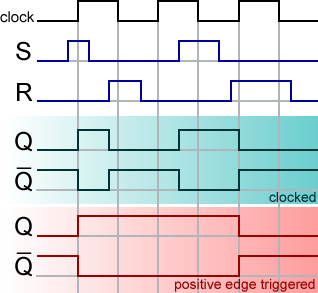
\includegraphics[width=28ex,trim=0 10pt 0 
%     0,clip]{SR_FF_timing_diagram.png}^^A
%   }^^A
%   \def\texta{ (left)}\def\textb{ (right)}^^A
%   }{}^^A
%  \def\exampleextraheader{%
%    \string\let
%    \string\insertoriginalimageforcomparisionifpresent\string\relax
%  }%
% \fi
% \begin{examplecode}
%   \definecolor{bgblue}{rgb}{0.41961,0.80784,0.80784}
%   \definecolor{bgred}{rgb}{1,0.61569,0.61569}
%   \definecolor{fgblue}{rgb}{0,0,0.6}
%   \definecolor{fgred}{rgb}{0.6,0,0}
%   \begin{tikztimingtable}[timing/slope=0,
%     timing/coldist=2pt,xscale=2,yscale=1.1,semithick]
%     \scriptsize clock & 7{C}\\
%     S & .75L h 2.25L H LLl [fgblue]\\
%     R & 1.8L .8H 2.2L 1.4H 0.8L [fgblue]\\
%     Q & L .8H 1.7L 1.5H LL\\
%     $\overline{\mbox{Q}}$ & H .8L 1.7H 1.5L HH\\
%     Q & LHHHHLL[fgred]\\
%     $\overline{\mbox{Q}}$ & HLLLLHH[fgred]\\
%   \extracode
%    \begin{pgfonlayer}{background}
%     \shade [right color=bgblue,left color=white]
%        (7,-8.45) rectangle (-2,-4.6);
%     \shade [right color=bgred,left color=white]
%        (7,-12.8) rectangle (-2,-8.6);
%     \begin{scope}[gray,semitransparent,semithick]
%       \horlines{}
%       \foreach \x in {1,...,6}
%         \draw (\x,1) -- (\x,-12.8);
%       % similar: \vertlines{1,...,6}
%     \end{scope}
%     \node [anchor=south east,inner sep=0pt]
%       at (7,-8.45) {\tiny clocked};
%     \node [anchor=south east,inner sep=0pt,fgred]
%       at (7,-12.8) {\tiny positive edge triggered};
%    \end{pgfonlayer}
%   \end{tikztimingtable}
%   \insertoriginalimageforcomparisionifpresent
% \end{examplecode}
% \caption[SR flip-flop timing diagram]{SR flip-flop timing diagram\texta.  
% Redrawn from image\textb\\ {\small
% \url{http://commons.wikimedia.org/wiki/File:SR_FF_timing_diagram.png}
% }}
% \end{example}
%
% \begin{example}
% \centering
% \lstset{basicstyle=\ttfamily\footnotesize}
% \def\texta{}\def\textb{}^^A
% \begin{examplecode}
%   \newcounter{countup}
%   \newcommand*{\countup}{\addtocounter{countup}{1}\thecountup}
%   \newcommand*{\crst}{\setcounter{countup}{0}}
%   \begin{tikztimingtable}
%     [timing/d/background/.style={fill=white},
%      timing/lslope=0.2]
%             CPOL=0 & LL 15{T} LL \\
%             CPOL=1 & HH 15{T} HH \\
%                    & H 17L H     \\
%     \\
%     \crst Cycle \# & U     8{2D{\countup}} 2U    \\
%     \crst     MISO & D{z}  8{2D{\countup}} 2D{z} \\
%     \crst     MOSI & D{z}  8{2D{\countup}} 2D{z} \\
%     \\
%     \crst Cycle \# & UU    8{2D{\countup}}  U    \\
%     \crst     MISO & D{z}U 8{2D{\countup}}  D{z} \\
%     \crst     MOSI & D{z}U 8{2D{\countup}}  D{z} \\
%   \extracode
%     \begin{pgfonlayer}{background}
%       \begin{scope}[semitransparent,semithick]
%         \vertlines[red]{2.1,4.1,...,17.1}
%         \vertlines[blue]{3.1,5.1,...,17.1}
%       \end{scope}
%     \end{pgfonlayer}
%     \begin{scope}
%       [font=\sffamily\Large,shift={(-6em,-0.5)},anchor=east]
%       \node at (  0, 0) {SCK};    \node at (  0,-3 ) {SS};
%       \node at (1ex,-9) {CPHA=0}; \node at (1ex,-17) {CPHA=1};
%     \end{scope}
%   \end{tikztimingtable}%
% \end{examplecode}
% \caption[SPI Interface Timing]{SPI Interface Timing\texta.  Redrawn from 
% image\textb\\ {\small
% \url{http://en.wikipedia.org/wiki/File:SPI_timing_diagram.svg}}}
% \end{example}
%
% \clearpage
% \StopEventually{}
% \clearpage
% \section{Implementation}
% \subsection{Package Header}
% \iffalse
%<*package>
% \fi
%    \begin{macrocode}
\RequirePackage{tikz}

\usetikzlibrary{calc}
\usetikzlibrary{backgrounds}
\usetikzlibrary{decorations.pathmorphing}
\ifx\collect@body\@undefined
  \IfFileExists{environ.sty}
    {\RequirePackage{environ}}
    {\RequirePackage{amsmath}}
\fi
%    \end{macrocode}
%
% \subsection{General Definitions}
%
%    \begin{macrocode}
\def\tikztimingwidth{0.0}
\newcount\tikztiming@numint
\newcount\tikztiming@numfrac
\def\tikztiming@wscale{1.0}%
\def\tikztimingsetwscale#1{%
  \pgfmathparse{#1}%
  \let\tikztiming@wscale\pgfmathresult
}
\def\tikztiming@num{0.0}%
\let\tikztiming@back\empty
\newlength\tikztiming@xunit
\newlength\tikztiming@yunit
\setlength{\tikztiming@xunit}{1.6ex}%
\setlength{\tikztiming@yunit}{1.6ex}%

\def\tikztiming@setnum#1{%
  \pgfmathparse{#1}%
  \global\let\tikztiming@num\pgfmathresult
}

\newcount\tikztiming@debug

\def\tikztiming@xsep{0pt}
\def\tikztiming@ysep{0pt}

\newcounter{tikztiming@nrows}%
\def\tikztiming@rowdist{2}%
\def\tikztiming@coldist{1}%

\def\tikztiming@prefix{tikztiming@trans@}%
\def\tikztiming@ttt#1#2#3{#1#2#3}%
\def\tikztiming@pfxtr{%
  \tikztiming@prefix\expandafter\tikztiming@ttt
}

\def\timingwidth{1}%
\def\timingheight{1}%
%    \end{macrocode}

% \subsection{TikZ Style Settings}
%    \begin{macrocode}
\tikzset{%
  timing/.style={%
    line cap=round, line join=round,
    timing/adjust@xy
  },%
}
\tikzset{%
  timing/.cd,
  adjust@xy/.style={%
    /utils/exec={%
      \tikz@textfont
      \setlength{\tikztiming@xunit}{1.6ex}%
      \setlength{\tikztiming@yunit}{1.6ex}%
    },%
    x=1.6ex, y=1.6ex,
  },
  font/.style={%
    /tikz/font={#1},
    /tikz/timing/adjust@xy
  },%
  initchar/.value required,
  initchar/.code={\uppercase{\gdef\tikztiming@lastchar{#1}}},
  metachar/.code={\tikztimingmetachar#1},
  grid/.style={timing,help lines},
  @grid/.code={\texttiminggrid},
  draw grid/.style={%
    timing/before text/.append style={timing/@grid},%
    timing/before/.append style={timing/@grid}%
  },
  no grid/.style={timing/@grid/.code={}},
  before/.code={},
  after/.code={},
  before text/.code={\texttimingbefore},
  after text/.code={\texttimingafter},
  picture/.style={timing,line width=0.15ex},
  intext/.style={timing,line width=0.15ex},
  inline node/.style={shape=coordinate},
  inline node/from char/.store in=\tikztiming@node@fromchar,
  inline node/to char/.store in=\tikztiming@node@tochar,
  table/.style={font=\sffamily,timing,line width=0.15ex},
  coord/.style={coordinate},
  save/.style={coordinate},
  restore/.style={/utils/exec={\expandafter\tikzset\expandafter{\tikztiming@saved@options}}},
  option/.style={/utils/exec={\g@addto@macro\tikztiming@saved@options{#1,}},#1},
  nooptions/.style={/utils/exec={\gdef\tikztiming@saved@options{}}},
  name/.style={inner sep=0pt,outer sep=0pt,minimum size=0pt},
  text format/.store in=\tikztiming@textformat,
  @/.style={},
  D/.style={timing/d},
  D/text/.style={timing/d/text},
  D/background/.style={timing/d/background},
  D@edge@/.style={timing/d@edge@},
  D@edge@/text/.style={timing/d@edge@/text},
  D@edge@/background/.style={timing/d@edge@/background},
  U/.style={timing/u},
  U/text/.style={timing/u/text},
  U/background/.style={timing/u/background},
  U@edge@/.style={timing/u@edge@},
  U@edge@/text/.style={timing/u@edge@/text},
  U@edge@/background/.style={timing/u@edge@/background},
  H/.style={timing/h},
  L/.style={timing/l},
  E/.style={timing/e},
  E/background/.style={timing/e/background},
  M/decoration/.style={timing/m/decoration},
  M/base/.style={timing/m/base},
  M/.style={timing/m},
  G/.style={timing/g},
  Z/.style={timing/z},
  T/.style={timing/t},
  C/.style={timing/c},
  X/.style={timing/x},
  d/.style={},
  d/text/.style={timing,scale=0.6,font=\sffamily},
  d/background/.style={draw=none},
  d@edge@/.style={timing/d},
  d@edge@/text/.style={timing/d/text},
  d@edge@/background/.style={timing/d/background},
  u/.style={},
  u/background/.style={draw=none,fill=gray},
  u@edge@/.style={timing/u},
  u@edge@/text/.style={timing/u/text},
  u@edge@/background/.style={timing/u/background},
  h/.style={},
  l/.style={},
  e/.style={},
  e/background/.style={draw=none},
  m/decoration/.style={decorate,%
    decoration={zigzag,segment length=.25\tikztiming@xunit,
    amplitude=.225\tikztiming@yunit}},
  m/base/.style={black!40!brown},
  m/.style={timing/m/base,timing/m/decoration},
  g/.style={decorate=false},
  z/.style={blue},
  t/.style={},
  c/.style={timing/lslope=0.0},
  x/.style={red},
  table/grid/.style={timing/grid},
  table/lines/.style={},
  table/rules/.style={line width=0.08em,line cap=butt},
  table/midrules/.style={line width=0.05em,line cap=butt},
  table/header/.style={timing/name},
  slope/.code={%
    \tikztimingsetslope{#1}%
    \tikztimingsetdslope{2*#1}%
    \tikztimingsetzslope{#1/2}%
  },
  lslope/.code={\tikztimingsetslope{#1}},
  dslope/.code={\tikztimingsetdslope{#1}},
  zslope/.code={\tikztimingsetzslope{#1}},
  wscale/.code={\tikztimingsetwscale{#1}},
  coldist/.store in=\tikztiming@coldist,
  rowdist/.store in=\tikztiming@rowdist,
  outer xsep/.store in=\tikztiming@xsep,
  outer ysep/.store in=\tikztiming@ysep,
  outer sep/.style={/tikz/timing/outer xsep=#1,/tikz/timing/outer ysep=#1},
}
\tikzset{timing/inline node/.cd,
  from char={}, to char={}
}
%    \end{macrocode}
%
% \subsection{Text-Mode Macros}
% \begin{macro}{\texttimingbefore}
% This macro is executed inside the |tikzpicture| environment of \cs{texttiming} 
% before the timing diagram is drawn.
%    \begin{macrocode}
\def\texttimingbefore{}
%    \end{macrocode}
% \end{macro}
%
% \begin{macro}{\texttimingafter}
% This macro is executed inside the |tikzpicture| environment of \cs{texttiming} 
% after the timing diagram is drawn.
%    \begin{macrocode}
\def\texttimingafter{}
%    \end{macrocode}
% \end{macro}
%
% \begin{macro}{\texttiminggrid}
% Draws a background grid with the `timing/grid' setting. Should be used inside 
% \cs{texttimingbefore}.
%    \begin{macrocode}
\def\texttiminggrid{%
  \draw[xstep={\timingwidth/2.},ystep={\timingheight/2.},timing/grid] (0,0) grid 
  (\timingwidth*\tikztimingwidth,\timingheight);
}
%    \end{macrocode}
% \end{macro}
%
% \subsection{User Level Macros}
%
% \begin{macro}{\texttiming}[2]{Optional initial character}{Timing characters}
% This macro now only parses it optional argument to check if it is a initial 
% character or some style settings and then calls \cs{timing} appropriately.
%    \begin{macrocode}
\DeclareRobustCommand*\texttiming[2][]{%
  \begingroup
    \let\tikztiming@lastchar\empty
    \let\tikztiming@settings\empty
    \tikzset{timing/before/.style={timing/before text}}%
    \tikzset{timing/after/.style={timing/after text}}%
    \ifx\relax#1\relax\else
      \tikztiming@testoptarg#1\relax\relax%
    \fi
    \begin{tikzpicture}[timing/intext,baseline={(0,0)}]
      \def\@tempa{\expandafter\timing\expandafter[\tikztiming@settings] at (0,0)}%
      \expandafter\@tempa\expandafter{\expandafter[\tikztiming@lastchar]#2};%
    \end{tikzpicture}%
  \endgroup
}
%    \end{macrocode}
% \end{macro}
%
% \begin{macro}{\tikztiming@testoptarg}
%    \begin{macrocode}
\def\tikztiming@testoptarg#1#2\relax{%
  \ifx\relax#2\relax
    \uppercase{\def\tikztiming@lastchar{#1}}%
  \else
    \def\tikztiming@settings{#1#2}%
  \fi
}
%    \end{macrocode}
% \end{macro}
%
% \begin{macro}{\tikztiming@init}
%    \begin{macrocode}
\def\tikztiming@init{%
    \def\tikztiming@lastchar{@}%
    \def\tikztiming@num{0}%
    \let\tikztiming@currentchar\empty
    \let\tikztiming@settings\empty
    \let\tikztiming@fromchar\empty
    \let\tikztiming@tochar\empty
    \let\setwscale\tikztimingsetwscale
    \def\wscale{\tikztiming@wscale}%
    \def\slope{\timingslope}%
    \def\lslope{\timingslope}%
    \def\zslope{\timingzslope}%
    \def\dslope{\timingdslope}%
    \gdef\tikztiming@saved@settings{}%
    \gdef\tikztiming@saved@options{}%
    \gdef\tikztiming@oldnodecenter@{}%
    \def\tikztimingwidth{0.0}%
    \setcounter{tikztimingtrans}{-1}%
    \setcounter{tikztimingtranspos}{0}%
    \def\tikztiming@str{%
      \useasboundingbox (0,0) rectangle (\tikztimingwidth,\timingheight);
      \draw (0,0)
        coordinate [shift={(0,\timingheight/2)}] (timing@ref)
        coordinate (timing/start base)
    }%
}
%    \end{macrocode}
% \end{macro}
%
% \begin{macro}{\tikz@timing}
%    \begin{macrocode}
\def\tikz@timing{%
  \@ifnextchar{[}%
    {\tikz@timing@}%
    {\tikz@timing@[]}%
}
%    \end{macrocode}
% \end{macro}
%
% \begin{macro}{\tikz@installcommands}
% Add \cs{timing} to the TikZ internal |\tikz@installcommands| macro.
% The |\timing| macro will be installed at the begin of the |tikzpicture|.
%    \begin{macrocode}
\g@addto@macro\tikz@installcommands{%
  \let\tikz@origtiming=\timing%
  \let\timing=\tikz@timing%
}
%    \end{macrocode}
% \end{macro}
%
% \begin{macro}{\tikz@uninstallcommands}
% Add \cs{timing} to the TikZ internal |\tikz@uninstallcommands| macro.
% The |\timing| macro will be uninstalled at the begin of nodes.
%    \begin{macrocode}
\g@addto@macro\tikz@uninstallcommands{%
  \let\timing=\tikz@origtiming%
}
%    \end{macrocode}
% \end{macro}
%
% \begin{macro}{\tikz@timing@}[1]{Optional TikZ Settings}
%    \begin{macrocode}
\def\tikz@timing@[#1]{%
  \@ifnextchar{a}%
    {\tikz@timing@at{#1}}%
    {\PackageWarning{tikz-timing}{The \string\timing\space command awaits now an 
    `at' before the coordinate, like the \string\node\space command is doing.  
    Please update your source code to ensure compatibility with newer 
    versions}{}{}{}%
     \@ifnextchar{+}%
      {\tikz@timing@@{#1}}%
      {\@ifnextchar(%)
        {\tikz@timing@@{#1}}%
        {\tikz@timing@@{#1}++(0,0)}%
      }%
    }%
}
%    \end{macrocode}
% \end{macro}
%
% \begin{macro}{\tikz@timing@at}[1]{Optional TikZ Settings}
%    \begin{macrocode}
\def\tikz@timing@at#1at#2(#3){%
  \tikz@timing@@@{#1}{#2(#3)}%
}
%    \end{macrocode}
% \end{macro}
%
% \begin{macro}{\tikz@timing@@}[3]{Optional TikZ Settings}{Potential `+' or 
% empty}{Coordinate}
%    \begin{macrocode}
\def\tikz@timing@@#1#2(#3){%
  \tikz@timing@@@{#1}{#2(#3)}%
}
%    \end{macrocode}
% \end{macro}
%
% \begin{macro}{\tikz@timing@@@}[3]{Optional TikZ Settings}{Coordinate}{Timing 
% Characters}
%    \begin{macrocode}
\def\tikz@timing@@@#1#2#3{%
  \begingroup
    \tikztiming@init
    \let\tikz@alias=\pgfutil@empty%
    \begin{scope}[shift={#2},timing,#1]%
      \@ifnextchar{[}%
        {\tikz@timing@@@init}%
        {\tikz@timing@@@init[]}%
      #3\relax
      \ifnum\tikztiming@debug>1
      \message{^^J\meaning\tikztiming@str^^J}%
      \ifnum\tikztiming@debug>2
      {%
      \def\@protect##1{\def##1{\noexpand##1}}%
      \@protect\useasboundingbox
      \@protect\draw
      \@protect\p
      \@protect\n
      \@protect\x
      \@protect\y
      \edef\@tempa{\tikztiming@str}%
      \message{^^J\meaning\@tempa^^J}%
      }%
      \fi
      \fi
      \tikzset{timing/before}%
      \tikztiming@str;%
      \node [shape=tikztiming@shape,anchor=origin,#1] at (0,0) {};
      \tikzset{timing/after}%
    \end{scope}%
  \endgroup
  \tikz@timing@@@end
}
%    \end{macrocode}
% \end{macro}
%
% \begin{macro}{\tikz@timing@@@end}
%    \begin{macrocode}
\def\tikz@timing@@@end{%
  \@ifnextchar{;}%
    {\@gobble}%
    {\PackageError{tikz-package}{Can not parse timing path}{}{}{}}%
}
%    \end{macrocode}
% \end{macro}
%
% \begin{macro}{\tikz@timing@@@init}[1]{Initial character.}
% Opens a group which will end in \cs{tikztiming@parser@end}.
%    \begin{macrocode}
\def\tikz@timing@@@init[#1]{%
  \begingroup
  \ifx\relax#1\relax\else
    \uppercase{\def\tikztiming@lastchar{#1}}%
  \fi
  \@ifundefined{tikztiming@initcode@\tikztiming@lastchar}%
    {}%
    {\@nameuse{tikztiming@initcode@\tikztiming@lastchar}}%
  \if @\tikztiming@lastchar\relax\else
  \tikztiming@iftrans{@\tikztiming@lastchar}%
    {\tikztiming@nameaddtostr{@}{\tikztiming@lastchar}{}}%
    {\PackageWarning{tikz-timing}{Start value for timing character 
    '\tikztiming@lastchar' is not defined and will be ignored!}{}{}{}}%
  \fi
  \tikztiming@parser
}
%    \end{macrocode}
% \end{macro}
%
% \subsection{Internal Macros}
%
% \begin{macro}{\tikztiming@trans@}
%    \begin{macrocode}
\def\tikztiming@trans@#1#2#3#4{%
  \csname\tikztiming@prefix #2#3#4\endcsname{#1}{#2}{#3}{#4}%
}
%    \end{macrocode}
% \end{macro}
%
% \begin{macro}{\tikztiming@beforenextcode@D@edge@}
%    \begin{macrocode}
\def\tikztiming@beforenextcode@D@edge@{%
  \if D\tikztiming@currentchar\else
    \gdef\tikztiming@lastchar{D}%
  \fi
}
%    \end{macrocode}
% \end{macro}
%
% \begin{macro}{\tikztiming@beforenextcode@U@edge@}
%    \begin{macrocode}
\def\tikztiming@beforenextcode@U@edge@{%
  \if U\tikztiming@currentchar\else
    \gdef\tikztiming@lastchar{U}%
  \fi
}
%    \end{macrocode}
% \end{macro}
%
% \begin{macro}{\tikztiming@initcode@}
% If empty init char was given, exchange it with `|@|'.
%    \begin{macrocode}
\def\tikztiming@initcode@{%
  \gdef\tikztiming@lastchar{@}%
}
%    \end{macrocode}
% \end{macro}
%
% \begin{macro}{\tikztiming@initcode@D}
%    \begin{macrocode}
\def\tikztiming@initcode@D{%
  \gdef\tikztiming@lastchar{D@edge@}%
}
%    \end{macrocode}
% \end{macro}
%
% \begin{macro}{\tikztiming@initcode@U}
%    \begin{macrocode}
\def\tikztiming@initcode@U{%
  \gdef\tikztiming@lastchar{U@edge@}%
}
%    \end{macrocode}
% \end{macro}
%
% \begin{macro}{\tikztiming@parser}
%    \begin{macrocode}
\def\tikztiming@parser{%
  \@ifnextchar\relax
    {\tikztiming@parser@end}%
    {\tikztiming@testfornum}%
}
%    \end{macrocode}
% \end{macro}
%
% \subsection{Add-to-Macro Macros}
% \begin{macro}{\tikztiming@eaddto}[2]{Macro name}{Tokens to add to macro}
%    \begin{macrocode}
\def\tikztiming@eaddto#1#2{%
  \begingroup
    \tikztiming@internaldefs
    \@temptokena\expandafter{#1}%
    \xdef#1{%
      \the\@temptokena
      #2%
    }%
  \endgroup
}
%    \end{macrocode}
% \end{macro}
%
%
% \begin{macro}{\tikztiming@eaddtostr}
%    \begin{macrocode}
\def\tikztiming@eaddtostr{%
  \tikztiming@eaddto\tikztiming@str
}
%    \end{macrocode}
% \end{macro}
%
% \begin{macro}{\tikztiming@addtostr}
%    \begin{macrocode}
\def\tikztiming@addtostr{%
  \g@addto@macro\tikztiming@str
}
%    \end{macrocode}
% \end{macro}
%
% \begin{macro}{\tikztiming@makeglobal}
%    \begin{macrocode}
\def\tikztiming@makeglobal#1{%
  \global\let#1#1\relax\relax
}
%    \end{macrocode}
% \end{macro}
%
% \begin{macro}{\tikztiming@iftrans}[1]{Characters}
%    \begin{macrocode}
\def\tikztiming@trans{}%
\def\tikztiming@iftrans#1{%
  \tikztiming@iftrans@#1\empty\empty\empty\relax
}
%    \end{macrocode}
% \end{macro}
%
% \begin{macro}{\tikztiming@iftrans}[4]
% {First character}{Second character}
% {Next character or empty}{Eats token till end marker}
%    \begin{macrocode}
\def\tikztiming@iftrans@#1#2#3#4\relax{%
  \begingroup
  \xdef\tikztiming@trans{#1#2}%
  \ifx\tikztiming@trans\empty
    \gdef\tikztiming@trans{{@}{}{@}}%
  \else
    \global\let\tikztiming@trans\relax
    % Use triple macros before double macros
    \@ifundefined{tikztiming@triple@#2}%
      {\@ifundefined{\tikztiming@prefix#1#2}%
        {}%
        {\xdef\tikztiming@trans{{#1}{#2}{}}}%
      }%
      {%
      \@ifundefined{\tikztiming@prefix#1#2#3}%
        {}%
        {\xdef\tikztiming@trans{{#1}{#2}{#3}}}%
      }%
    % If both do not exist, search for aliases:
    \ifx\tikztiming@trans\relax
      \@ifundefined{tikztiming@alias@#1}%
        {\edef\chara{#1}}%
        {\edef\chara{#1,\csname tikztiming@alias@#1\endcsname}}%
      \@ifundefined{tikztiming@alias@#2}%
        {\edef\charb{#2}}%
        {\edef\charb{#2,\csname tikztiming@alias@#2\endcsname}}%
      \@ifundefined{tikztiming@triple@#2}%
        {\def\charc{\empty}}%
        {%
         \@ifundefined{tikztiming@alias@#3}%
           {\edef\charc{#3,}}%
           {\edef\charc{#3,\csname tikztiming@alias@#3\endcsname,}}%
        }%
      \ifx\charb\empty
        \def\charb{\empty}%
      \fi
      \let\tikztiming@next\relax
      \foreach \b in \charb {%
        \foreach \a in \chara {%
          \foreach \c in \charc {%
            %\message{ ^^J Testing: \a\b\c ^^J}%
            \@ifundefined{\tikztiming@prefix\a\b\c}%
              {}{%
                \xdef\tikztiming@trans{{#1}{#2}{#3}}%
                \expandafter\tikztimingcpy\expandafter
                  {\tikztiming@trans}{\a\b\c}%
                \ifnum\tikztiming@debug>0
                  \message{^^J DEBUG: '#1#2#3' = '\a\b\c' ^^J}%
                \fi
                \expandafter\tikztiming@makeglobal
                \csname\tikztiming@pfxtr\tikztiming@trans\endcsname
                \ifnum\tikztiming@debug>1
                  \ifnum\tikztiming@debug>2
                    \expandafter\show\csname\tikztiming@pfxtr\tikztiming@trans\endcsname
                  \else
                    \message{^^J\tikztiming@trans: 
                    \expandafter\meaning\csname\tikztiming@pfxtr\tikztiming@trans\endcsname^^J}%
                    \message{^^J\a\b\c: 
                    \expandafter\meaning\csname\tikztiming@prefix\a\b\c\endcsname^^J}%
                  \fi
                \fi
                \global\let\tikztiming@next\breakforeach
              }%
            \tikztiming@next
          }%
          \tikztiming@next
        }%
        \tikztiming@next
      }%
    \fi
  \fi
  \endgroup
  \ifx\tikztiming@trans\relax
    \expandafter\@secondoftwo
  \else
    \expandafter\@firstoftwo
  \fi
}
%    \end{macrocode}
% \end{macro}
%
% \begin{macro}{\tikztiming@nameaddtostr}
% {First character}{Second character}
% {Optional next character}
%    \begin{macrocode}
\def\tikztiming@nameaddtostr#1#2#3{%
  \tikztiming@iftrans{{#1}{#2}{#3}}%
   {%
     \edef\@tempa{\noexpand\tikztiming@trans@{\tikztiming@num}\tikztiming@trans}%
     \expandafter\g@addto@macro
     \expandafter\tikztiming@str
     \expandafter{\@tempa}%
   }%
   {\PackageWarning{tikz-timing}{No transitions '#1#2' (or '#1#2#3') defined!}}%
}
%    \end{macrocode}
% \end{macro}
%
% \begin{macro}{\tikztiming@output@addcode}
% Adds code to the output code buffer. The code will not be expanded, i.e.\ will 
% be protected from the expansion when the buffer is flushed.
%    \begin{macrocode}
\def\tikztiming@output@addcode#1{%
  \g@addto@macro\tikztiming@output@bufcode{\unexpanded{ #1 }}%
}
%    \end{macrocode}
% \end{macro}
%
% \begin{macro}{\tikztiming@output@eaddcode}
% Adds code to the output code buffer. The code will be expanded when the buffer 
% is flushed.
%    \begin{macrocode}
\def\tikztiming@output@eaddcode#1{%
  \g@addto@macro\tikztiming@output@bufcode{ #1 }%
}
%    \end{macrocode}
% \end{macro}
%
% \begin{macro}{\tikztiming@output@Eaddcode}
% Adds code to the output code buffer. The code will be expanded immediately and 
% again when the buffer is flushed.
%    \begin{macrocode}
\def\tikztiming@output@Eaddcode{%
  \tikztiming@eaddto\tikztiming@output@bufcode%
}
%    \end{macrocode}
% \end{macro}
%
%
% \subsection{Output Routine}
%
% Init buffer macros:
%    \begin{macrocode}
\def\tikztiming@output@bufchara{}%
\def\tikztiming@output@bufcharb{}%
\def\tikztiming@output@bufnum{0}%
\def\tikztiming@output@bufcode{}%
\def\tikztiming@output@nextchar{}%
%    \end{macrocode}
%
% \begin{macro}{\tikztiming@output}[2]{Character 1}{Character 2}
%    \begin{macrocode}
\def\tikztiming@output#1#2{%
  \edef\tikztiming@fromchar{#1}%
  \edef\tikztiming@tochar{#2}%
  \ifx\relax#2\relax
    %\tikztiming@output@codeflush
    \tikztiming@nameaddtostr{}{#1}{}%
  \else
    \ifcase0%
      \ifx\tikztiming@output@bufchara\empty
        \ifx\tikztiming@output@bufcharb\empty
          1%
        \fi
      \fi\relax
      % not empty
      \edef\tikztiming@output@currentchar{#2}%
      \ifcase0%
       \ifx\tikztiming@output@bufcode\empty% Stop combining if code was inserted
        \expandafter\ifx\csname tikztiming@nocombine@#2\endcsname\relax
         \ifx\tikztiming@output@currentchar\tikztiming@output@bufcharb
           2%
         \fi
        \fi
       \else
         1%
       \fi
      \relax
        \edef\tikztiming@output@nextchar{#2}%
        \tikztiming@output@flush
        \xdef\tikztiming@output@bufchara{#1}%
        \xdef\tikztiming@output@bufcharb{#2}%
      \or
        \edef\tikztiming@output@nextchar{#2}%
        \tikztiming@output@flush
        \xdef\tikztiming@output@bufchara{#1}%
        \xdef\tikztiming@output@bufcharb{#2}%
      \or
        \pgfmathparse{\tikztiming@output@bufnum + \tikztiming@num}%
        \global\let\tikztiming@output@bufnum\pgfmathresult
      \fi
    \else % empty
      \tikztiming@output@codeflush
      \xdef\tikztiming@output@bufchara{#1}%
      \xdef\tikztiming@output@bufcharb{#2}%
      \global\let\tikztiming@output@bufnum\tikztiming@num
    \fi
  \fi
}
%    \end{macrocode}
% \end{macro}
%
% \begin{macro}{\tikztiming@output@flush}
%    \begin{macrocode}
\def\tikztiming@output@flush{%
  \tikztiming@output@charflush
  \tikztiming@output@codeflush
}
%    \end{macrocode}
% \end{macro}
%
% \begin{macro}{\tikztiming@output@codeflush}
%    \begin{macrocode}
\def\tikztiming@output@codeflush{%
  \tikztiming@eaddtostr{\tikztiming@output@bufcode}%
  \global\let\tikztiming@output@bufcode\empty%
}
%    \end{macrocode}
% \end{macro}
%
% \begin{macro}{\tikztiming@output@charflush}
% A group is used to protect the current value of |num| which is the length of 
% the new character after the flushed old character. This value will be assigned 
% to the new buffer length |bufnum|.
%    \begin{macrocode}
\def\tikztiming@output@charflush{%
  \begingroup
    \let\tikztiming@num\tikztiming@output@bufnum
    \tikztiming@nameaddtostr
      {\tikztiming@output@bufchara}%
      {\tikztiming@output@bufcharb}%
      {\tikztiming@output@nextchar}%
  \endgroup%
  \gdef\tikztiming@output@nextchar{}%
  \gdef\tikztiming@output@bufchara{}%
  \gdef\tikztiming@output@bufcharb{}%
  \global\let\tikztiming@output@bufnum\tikztiming@num
}
%    \end{macrocode}
% \end{macro}
%
%
% \subsection{Macros for Character Definitions}
%
% \begin{macro}{\tikztiming@nameedef}[4]{Macro name to be defined (without 
% prefix)}{Content of macro}
% Defines internal tikztiming macro with name |\|\meta{prefix}\meta{name (\#2)}.  
% The macro definition (\#3) is expanded while the internal drawing definitions 
% are active.
%    \begin{macrocode}
\newcommand\tikztiming@nameedef[4]{%
  \def\@gtempa##1{#4}%
  \begingroup
    \tikztiming@internaldefs
    \xdef\@gtempa##1##2##3##4{\@gtempa{\width}}%
  \endgroup
  \expandafter\let\csname\tikztiming@prefix#1#2#3\endcsname\@gtempa
  \let\@gtempa\empty
}
%    \end{macrocode}
% \end{macro}
%
% \begin{macro}{\tikztiming@namelet}[2]{Original Characters}{New Characters}
% Only execute |\let| if the original macro is defined or the destination macro 
% is defined and would now set to undefined.
%    \begin{macrocode}
\newcommand\tikztiming@namelet[2]{%
  \ifcase0%
    \@ifundefined{\tikztiming@prefix#2}%
      {\@ifundefined{\tikztiming@prefix#1}%
        {0}{1}%
      }%
      {1}%
    \relax
  \else
    \expandafter\let
    \csname\tikztiming@prefix#1\expandafter\endcsname
    \csname\tikztiming@prefix#2\endcsname
  \fi
}
%    \end{macrocode}
% \end{macro}
%
%
% \subsection{Parser}
%
% \begin{macro}{\tikztiming@parser@end}
%    \begin{macrocode}
\def\tikztiming@parser@end{%
  \def\tikztiming@output@nextchar{@}%
  \let\tikztiming@fromchar\tikztiming@tochar
  \edef\tikztiming@tochar{@}%
  \tikztiming@output@flush
  \global\let\tikztimingwidth\tikztimingwidth
  \tikztiming@addtostr{ coordinate (timing/end)
    let \p1 = (timing/start base), \p2 = (timing/end) in
      coordinate (timing/end base) at (\x2,\y1)
      coordinate (timing/end top)  at (\x2,1+\y1)
  }%
  \endgroup
  \tikztiming@endhook%
}
\let\tikztiming@endhook\relax
%    \end{macrocode}
% \end{macro}
%
% \begin{macro}{\tikztiming@parser@}[1]{Next Character}
%    \begin{macrocode}
\def\tikztiming@parser@#1{%
  \ifx\relax#1\empty
    \expandafter\tikztiming@parser@end
  \else
    \tikztiming@iflower{#1}%
      {\tikztiming@setnum{\tikztiming@num/2}}%
      {}%
    \ifx\tikztiming@back\empty\else
      \tikztiming@setnum{\tikztiming@num - \tikztiming@back}%
      \global\let\tikztiming@back\empty
    \fi
    \pgfmathparse{\tikztimingwidth + \tikztiming@num}%
    \global\let\tikztimingwidth\pgfmathresult
    \uppercase{\gdef\tikztiming@currentchar{#1}}%
    \@nameuse{tikztiming@beforenextcode@\tikztiming@lastchar}%
    \@nameuse{tikztiming@beforecode@\tikztiming@currentchar}%
    \tikztiming@output{\tikztiming@lastchar}{\tikztiming@currentchar}%
    \global\let\tikztiming@lastchar\tikztiming@currentchar
    \@nameuse{tikztiming@aftercode@\tikztiming@currentchar}%
    \expandafter
    \tikztiming@testfortext
  \fi
}
%    \end{macrocode}
% \end{macro}
%
% \begin{macro}{\tikztiming@testfortext}
%    \begin{macrocode}
\def\tikztiming@testfortext{%
  \@ifnextchar\bgroup
    {\tikztiming@handletext}%
    {\tikztiming@parser}%
}
%    \end{macrocode}
% \end{macro}
%
% \begin{macro}{\tikztiming@handletext}[1]{Text}
% Looks ahead if the current character is the last one and sets the end-of-line 
% marker if so. 
%
% This seems outdated because |handletext@| does not flush the output any more.
%     \begin{macrocode}
\def\tikztiming@handletext#1{%
  \@ifnextchar\relax
    {\def\tikztiming@output@nextchar{@}\tikztiming@handletext@{#1}}%
    {\def\tikztiming@output@nextchar{Z}\tikztiming@handletext@{#1}}%
}
%    \end{macrocode}
% \end{macro}
%
% \begin{macro}{\tikztiming@handletext@}[1]{Text}
%    \begin{macrocode}
\def\tikztiming@handletext@#1{%
  \@ifnextchar{[}%
    {\tikztiming@handletext@@}%
    {\tikztiming@handletext@@[]}%
  #1\tikztiming@endoftext
}
%    \end{macrocode}
% \end{macro}
%
% \begin{macro}{\tikztiming@handletext@@}[2]{Optional Settings}{Text}
%    \begin{macrocode}
\def\tikztiming@handletext@@[#1]#2\tikztiming@endoftext{%
  \@ifnextchar{\relax}%
    {\def\tikztiming@output@nextchar{@}%
     \tikztiming@handletext@@@{#1}{#2}}%
    {\tikztiming@handletext@@@{#1}{#2}}%
}
%    \end{macrocode}
% \end{macro}
%
% \begin{macro}{\tikztiming@handletext@@@}[2]{Optional Settings}
% {Text}
%    \begin{macrocode}
\def\tikztiming@handletext@@@#1#2{%
  \expandafter\lowercase\expandafter{%
    \expandafter\def\expandafter\@tempa
    \expandafter{\tikztiming@currentchar}%
  }%
  \pgfkeysifdefined{/tikz/timing/\@tempa/text/.@cmd}%
  {%
    \edef\@tempa{node [timing/\@tempa/text,}%
    \expandafter\tikztiming@output@addcode\expandafter{%
      \@tempa
      #1] at ($ (timing@dstart) !.5! (timing@dend) $)
      {\tikztiming@textformat{#2}}
    }%
    \ifcase0%
      \if @\tikztiming@output@bufchara
        1%
      \else
        \ifx\tikztiming@output@bufchara\tikztiming@currentchar
          1%
        \fi
      \fi
    \relax
    \else
    \fi
    \xdef\tikztiming@output@bufcharb{\tikztiming@currentchar @edge@}%
    \xdef\tikztiming@lastchar{\tikztiming@currentchar @edge@}%
  }{%
    \endgroup
    \PackageWarning{tikz-timing}{Ignoring text for character 
    '\tikztiming@currentchar'!}{}{}{}%
  }%
  \tikztiming@parser
}
\let\tikztiming@textformat\empty
%    \end{macrocode}
% \end{macro}
%
% \subsection{Definition of Modifiers}
%
% \begin{macro}{\tikztiming@defcode}[1]{Code Character}
%    \begin{macrocode}
\def\tikztiming@defcode#1{%
  \@namedef{tikztiming@code@\meaning#1}%
}
%    \end{macrocode}
% \end{macro}
%
% \begin{macro}{\tikztiming@defcode{@}}
% Simply executes given code. The |\relax| is added to have some protection 
% against user code manipulating the parser macro. The `@' character can be both 
% a letter (in style files) and a character (in user documents), so it is
% defined twice.
%    \begin{macrocode}
\tikztiming@defcode{@}#1{%
  #1\relax
  \tikztiming@parser
}
\begingroup
  \expandafter\let\expandafter\temp
    \csname tikztiming@code@\meaning @\endcsname
  \makeatother
  \expandafter\global\expandafter\let
    \csname tikztiming@code@\meaning @\endcsname\temp
\endgroup
%    \end{macrocode}
% \end{macro}
%
% \begin{macro}{\tikztiming@defcode{DOLLAR}}
% Takes the code between two dollar signs and parses it as math expression. The 
% result is put back on the input stream. This allows the calculation of 
% character width.
%    \begin{macrocode}
\tikztiming@defcode$#1${%
  \pgfmathparse{#1}%
  \expandafter
  \tikztiming@parser\pgfmathresult
}
%    \end{macrocode}
% \end{macro}
%
% \begin{macro}{\tikztiming@defcode{,}}
%    \begin{macrocode}
\tikztiming@defcode{,}{%
  \tikztiming@output@eaddcode{%
    \newdraw
  }%
  \tikztiming@parser
}
%    \end{macrocode}
% \end{macro}
%
% \begin{macro}{\tikztiming@defcode{;}}
%    \begin{macrocode}
\tikztiming@defcode{;}{%
  \endgroup\begingroup
  \tikztiming@output@eaddcode{%
    \newdrawns
  }%
  \tikztiming@parser
}
%    \end{macrocode}
% \end{macro}
%
% \begin{macro}{\tikztiming@defcode{N}}
%    \begin{macrocode}
\tikztiming@defcode{N}{%
  \@ifnextchar[%]
    {\tikztiming@addnode@getoptions}%
    {\tikztiming@addnode@getoptions[]}%
}
%    \end{macrocode}
% \end{macro}
%
% \begin{macro}{\tikztiming@defcode{n}}
%    \begin{macrocode}
\tikztiming@defcode{n}{%
  \@ifnextchar[%]
    {\tikztiming@addnode@getoptions}%
    {\tikztiming@addnode@getoptions[]}%
}
%    \end{macrocode}
% \end{macro}
%
% \begin{macro}{\tikztiming@defcode{B}}
%    \begin{macrocode}
\tikztiming@defcode{B}{%
  \pgfmathparse{\tikztiming@back+\tikztiming@num}%
  \global\let\tikztiming@back\pgfmathresult
  \tikztiming@parser
}
%    \end{macrocode}
% \end{macro}
%
% \begin{macro}{\tikztiming@defcode{b}}
%    \begin{macrocode}
\tikztiming@defcode{b}{%
  \pgfmathparse{\tikztiming@back+\tikztiming@num/2}%
  \global\let\tikztiming@back\pgfmathresult
  \tikztiming@parser
}
%    \end{macrocode}
% \end{macro}
%
% \begin{macro}{\tikztiming@defcode{F}}
%    \begin{macrocode}
\tikztiming@defcode{F}{%
  \pgfmathparse{\tikztiming@back-\tikztiming@num}%
  \global\let\tikztiming@back\pgfmathresult
  \tikztiming@parser
}
%    \end{macrocode}
% \end{macro}
%
% \begin{macro}{\tikztiming@defcode{f}}
%    \begin{macrocode}
\tikztiming@defcode{f}{%
  \pgfmathparse{\tikztiming@back-\tikztiming@num/2}%
  \global\let\tikztiming@back\pgfmathresult
  \tikztiming@parser
}
%    \end{macrocode}
% \end{macro}
%
%
% \begin{macro}{\tikztiming@defcode []}[1]{Options}
% Single brackets are in-picture options.
% Brackets and a `|!|' sign `|[! !]|' are parser options.
% Double brackets are are both.
%    \begin{macrocode}
\tikztiming@defcode[{%}]{
  \@ifnextchar[%]
    {\tikztiming@bothoption}%
    {\@ifnextchar{!}%
      {\tikztiming@parseroption}%
      {\tikztiming@addoption}%
    }%
}
%    \end{macrocode}
% \end{macro}
%
% \begin{macro}{\tikztiming@parseroption}[1]{Options}
% Sets the given options immediately, so that they are in affect for the rest of 
% the parser run.
%    \begin{macrocode}
\def\tikztiming@parseroption!#1!]{%
  \pgfqkeys{/tikz/timing}{#1}%
  \tikztiming@parser
}
%    \end{macrocode}
% \end{macro}
%
% \begin{macro}{\tikztiming@addoption}[1]{Options}
% Simply adds the options to the output code buffer.
%    \begin{macrocode}
\def\tikztiming@addoption#1]{%
  \tikztiming@output@addcode{ [timing/option={#1}] }%
  \tikztiming@parser
}
%    \end{macrocode}
% \end{macro}
%
% \begin{macro}{\tikztiming@bothoption}[1]{Options}
% Does executes and adds the options to the output code buffer. This is 
% necessary for slopes if they are used in width calculations.
%    \begin{macrocode}
\def\tikztiming@bothoption[#1]]{%
  \tikzset{#1}%[
  \tikztiming@addoption{#1}]%
}
%    \end{macrocode}
% \end{macro}
%
% \subsubsection{Add-Node Macros}
%
% \begin{macro}{\tikztiming@addnode}[1]{Options}
%    \begin{macrocode}
\def\tikztiming@addnode@getoptions[#1]{%
  \@ifnextchar(%)
    {\tikztiming@addnode@getname{#1}}%
    {\tikztiming@addnode@getname{#1}()}%
}
%    \end{macrocode}
% \end{macro}
%
% \begin{macro}{\tikztiming@addnode@getname}[2]{Previous read options}{Node 
% name}
%    \begin{macrocode}
\def\tikztiming@addnode@getname#1(#2){%
  \@ifnextchar\bgroup
    {\tikztiming@addnode@{#1}{#2}}%
    {\tikztiming@addnode@{#1}{#2}{}}%
}
%    \end{macrocode}
% \end{macro}
%
% \begin{macro}{\tikztiming@addnode@}[3]{Options}{Node name}{Node text}
% The |fromchar| and |tochar| macros are to be expanded in the output routine, 
% not inside this macro. They do not hold the correct values yet.
%    \begin{macrocode}
\def\tikztiming@addnode@#1#2#3{%
  \def\@tempa{#2}%
  \ifx\@tempa\empty
    \def\@tempa{ node [timing/inline node,%
      timing/inline node/from char={\tikztiming@fromchar},%
      timing/inline node/to char={\tikztiming@tochar},%
      \unexpanded{#1}] }%
  \else
    \def\@tempa{ node [timing/inline node,%
      timing/inline node/from char={\tikztiming@fromchar},%
      timing/inline node/to char={\tikztiming@tochar},%
      \unexpanded{#1}] (\unexpanded{#2}) }%
  \fi
  \expandafter\tikztiming@output@eaddcode\expandafter{\@tempa \unexpanded{{#3}} 
  }%
  \tikztiming@parser
}
%    \end{macrocode}
% \end{macro}
%
% \subsubsection{Test for Code (`!' modifier)}
%
% \begin{macro}{\tikztiming@testforcode}
%    \begin{macrocode}
\def\tikztiming@testforcode{%
  \@ifnextchar{!}%
    {\tikztiming@testforcode@}%
    {\@ifundefined{tikztiming@code@\meaning\@let@token}%
      {\tikztiming@parser@}%
      {\expandafter\afterassignment
       \csname tikztiming@code@\meaning\@let@token\endcsname
       \let\@let@token=%
      }%
    }%
}
%    \end{macrocode}
% \end{macro}
%
% \begin{macro}{\tikztiming@testforcode@}[1]{Character to gobble}
%    \begin{macrocode}
\def\tikztiming@testforcode@#1{%
  \@ifnextchar\bgroup
    {\tikztiming@handlecode}%
    {%
      \PackageWarning{tikz-timing}{Missing braces after '!' character. Ignoring 
      this character}{}{}{}%
      \tikztiming@parser
    }%
}
%    \end{macrocode}
% \end{macro}
%
% \begin{macro}{\tikztiming@handlecode}[1]{Code to add to string}
%    \begin{macrocode}
\def\tikztiming@handlecode#1{%
  \tikztiming@output@addcode{ #1 }%
  \tikztiming@parser
}
%    \end{macrocode}
% \end{macro}
%
%
% \subsection{Parser Macros: Numbers}
%
% \begin{macro}{\tikztiming@testfornum}
%    \begin{macrocode}
\def\tikztiming@testfornum{%
  \global\let\tikztiming@num\tikztiming@wscale
  \let\tikztiming@numchars\empty
  \tikztiming@numfrac0\relax
  \afterassignment
  \tikztiming@testfornum@
  \tikztiming@numint0%
}
%    \end{macrocode}
% \end{macro}
%
% \begin{macro}{\tikztiming@testfornumfrac}
%    \begin{macrocode}
\def\tikztiming@testfornumfrac{%
  \afterassignment
  \tikztiming@testfornum@@@
  \tikztiming@numfrac1%
}
%    \end{macrocode}
% \end{macro}
%
% \begin{macro}{\tikztiming@numloop}
%    \begin{macrocode}
\def\tikztiming@numloop{%
  \ifnum\tikztiming@numint>0%
    \toks@\expandafter{\tikztiming@numchars}%
    \xdef\tikztiming@numchars{%
      \the\toks@
      \the\@temptokena
    }%
    \advance\tikztiming@numint by -1\relax
    \expandafter\tikztiming@numloop
  \fi
}
%    \end{macrocode}
% \end{macro}
%
% \begin{macro}{\tikztiming@testfornum@}
% The \cs{@let@token} set in \cs{tikztiming@parser} is used to handle `|0|' 
% which can not be detected using the \cs{tikztiming@numint} value.
%    \begin{macrocode}
\def\tikztiming@testfornum@{%
  \ifx0\@let@token
    \let\tikztiming@next\tikztiming@testfornum@@
  \else
  \ifnum0<\tikztiming@numint
    \let\tikztiming@next\tikztiming@testfornum@@
  \else
    \def\tikztiming@next{%
      \@ifnextchar{.}%
        {\expandafter\tikztiming@testfornumfrac\@gobble}%
        {%
          \tikztiming@numint1\relax
          \tikztiming@numfrac0\relax
          \global\let\tikztiming@num\tikztiming@wscale
          \if@tikztiming@metachar
            {\def\@tempa{\expandafter\expandafter\expandafter
             \tikztiming@parser
             \csname tikztiming@metachar@\meaning\@let@token\endcsname{1}}%
             \expandafter\@tempa\@gobble
            }%
            {\tikztiming@testforcode}%
        }%
    }%
  \fi\fi
  \tikztiming@next
}
%    \end{macrocode}
% \end{macro}
%
% \begin{macro}{\tikztiming@testfornum@@}
%    \begin{macrocode}
\def\tikztiming@testfornum@@{%
  \@ifnextchar{.}%
    {\expandafter\tikztiming@testfornumfrac\@gobble}%
    {\tikztiming@testfornum@@@}%
}
%    \end{macrocode}
% \end{macro}
%
% \begin{macro}{\tikztiming@testfornum@@@}
%    \begin{macrocode}
\def\tikztiming@testfornum@@@{%
  \edef\tikztiming@num{\the\tikztiming@numint.\expandafter\@gobble\the\tikztiming@numfrac}%
  \tikztiming@setnum{\tikztiming@wscale * \tikztiming@num}%
  \@ifnextchar\bgroup
    {%
      \expandafter\tikztiming@numfrac\expandafter0\expandafter
      \@gobble\the\tikztiming@numfrac\relax
      \ifnum0=\tikztiming@numfrac\else
        \pgfmathparse{round(\tikztiming@num)}%
        \PackageWarning{tikz-timing}%
          {Can not repeat group by a non-integer factor!^^J%
           Rounding '\tikztiming@num' to '\pgfmathresult'.}{}{}{}%
        \global\let\tikztiming@num\pgfmathresult
      \fi
      \tikztiming@testfornum@@@@
    }%
    {%
      \if@tikztiming@metachar
        {\def\@tempa{\expandafter\expandafter\expandafter
        \tikztiming@parser
        \csname tikztiming@metachar@\meaning\@let@token\expandafter\endcsname
        \expandafter{\tikztiming@num}}%
        \expandafter\@tempa\@gobble
        }%
        {\tikztiming@testforcode}%
    }%
}
%    \end{macrocode}
% \end{macro}
%
% \begin{macro}{\tikztiming@testfornum@@@@}[1]{Characters and other tokens to 
% repeat}
%    \begin{macrocode}
\def\tikztiming@testfornum@@@@#1{%
  \begingroup
    \@temptokena{#1}%
    \tikztiming@numloop%
  \endgroup
  \tikztiming@numint1\relax
  \tikztiming@numfrac0\relax
  \expandafter\tikztiming@parser\tikztiming@numchars
}
%    \end{macrocode}
% \end{macro}
%
% \subsection{Macro Characters}
%
% \begin{macro}{\tikztimingmetachar}[1]{Macro character}
% Checks if there is an optional argument and calls \cs{tikztiming@metachar} 
% appropriately.
%    \begin{macrocode}
\def\tikztimingmetachar#1{%
  \@ifnextchar{[}%]
    {\tikztiming@metachar{#1}}%
    {\tikztiming@metachar{#1}[]}%
}
%    \end{macrocode}
% \end{macro}
%
% \begin{macro}{\tikztiming@metachar}[3]{Macro character}{Number of 
% Arguments}{Substituted Characters}
%    \begin{macrocode}
\def\tikztiming@metachar#1[#2]#3{%
  \ifx\relax#3\relax
    \expandafter\let\csname tikztiming@metachar@\meaning#1\endcsname\@undefined
  \else
    \@namedef{tikztiming@metachar@\meaning#1}{}%
    \ifx\relax#2\relax
      \expandafter\renewcommand\expandafter*%
      \csname tikztiming@metachar@\meaning#1\expandafter
      \endcsname\expandafter[1]{##1{#3}}%
    \else
      \expandafter\renewcommand\expandafter*%
      \csname tikztiming@metachar@\meaning#1\expandafter
      \endcsname\expandafter[#2]{#3}%
    \fi
  \fi
}
%    \end{macrocode}
% \end{macro}
%
% \begin{macro}{\if@tikztiming@metachar}[2]{True clause}{False clause}
% Only works in an argument of |\@ifnextchar|. This macro sets the needed 
% |\@let@token| macro.
%    \begin{macrocode}
\def\if@tikztiming@metachar#1#2{%
  \@ifundefined{tikztiming@metachar@\meaning\@let@token}{#2}{#1}%
}
%    \end{macrocode}
% \end{macro}
%
% \subsection{Table environment}
%    \begin{macrocode}
%\usetikzlibrary{backgrounds}
\newcounter{tikztimingrows}
%    \end{macrocode}
%
% \begin{macro}{\tikztiming@extracode}
%    \begin{macrocode}
\def\tikztiming@extracode{\@gobble{EXTRACODE}}%
%    \end{macrocode}
% \end{macro}

% \begin{environment}{tikztimingtable}[1]{Optional settings}
%    \begin{macrocode}
\newenvironment{tikztimingtable}[1][]{%
  \begingroup
  \setcounter{tikztiming@nrows}{0}%
  \def\tikztiming@maxwidth{0.0}%
  \let\extracode\tikztiming@extracode
  \let\tablegrid\tikztiming@tablegrid
  \let\fulltablegrid\tikztiming@fulltablegrid
  \let\horlines\tikztiming@horlines
  \let\vertlines\tikztiming@vertlines
  \def\tablerules{\tikztiming@tablerules}%
  \def\tableheader{\tikztiming@tableheader}%
  \def\rowdist{\tikztiming@rowdist}%
  \def\coldist{\tikztiming@coldist}%
  \def\nrows{\the\c@tikztiming@nrows}%
  \def\twidth{\tikztiming@maxwidth}%
  \tikzpicture[timing/table,#1]%
    \coordinate (last row)  at (0,\rowdist);
    \coordinate (label pos) at (-1*{(\coldist)},0);
    \coordinate (timing/table/top left) at (0,1);
    \coordinate (timing/table/bottom right) at (0,0);
  \collect@body\tikztiming@table
}{%
}
%    \end{macrocode}
% \end{environment}

% \begin{macro}{\tikztiming@table}[1]{Table content}
%    \begin{macrocode}
\def\tikztiming@table#1{%
  \tikztimingtable@row#1\endtikztimingtable@
  \endtikzpicture
  \endgroup
}
%    \end{macrocode}
% \end{macro}

% \begin{macro}{\endtikztimingtable@}
%    \begin{macrocode}
\def\endtikztimingtable@{\@gobble{ENDTIKSTIMING}}
%    \end{macrocode}
% \end{macro}

% \begin{macro}{\tikztiming@extracode}[2]{Token to gobble}{Extra drawing code}
%    \begin{macrocode}
\long\def\tikztiming@extracode#1#2\endtikztimingtable@{%
  \path let
     \p1 = (timing/table/top left),
     \p2 = (timing/table/bottom right)
   in
     coordinate (timing/table/bottom left) at (\x1,\y2)
     coordinate (timing/table/top right) at (\x2,\y1)
     coordinate (timing/table/size) at (\x2-\x1,\y1-\y2)
   ;
  #2%
}
%    \end{macrocode}
% \end{macro}
%
% \begin{macro}{\tikztiming@emptycell}
% Just used as marker. Needs unique definition.
%    \begin{macrocode}
\def\tikztiming@emptycell{%
  \@gobble{tikztiming@emptycell}%
}
%    \end{macrocode}
% \end{macro}
%
% \begin{macro}{\tikztimingtable@row}[1]{Row content}
%    \begin{macrocode}
\def\tikztimingtable@row#1\\{%
  \tikztimingtable@row@#1&\tikztiming@emptycell&\\
}
%    \end{macrocode}
% \end{macro}
%
% \begin{macro}{\tikztimingtable@row@}[3]{Cell 1}{Cell 2 or empty}{Potential 
% further cells}
%    \begin{macrocode}
\def\tikztimingtable@row@#1&#2&#3\\{%
  \ifx\\#3\\\else
    \begingroup
      \def\@tempa{\tikztiming@emptycell&}%
      \def\@tempb{#3}%
      \ifx\@tempa\@tempb\else
        \PackageWarning{tikz-timing}{%
          To many columns in tikztimingtable row! Only two are allowed%
        }{}{}{}%
      \fi
    \endgroup
  \fi
  \ifx\tikztiming@emptycell#2%
    \def\tikztiming@next{\tikztimingtable@row@@{#1}{}}%
  \else
    \def\tikztiming@next{\tikztimingtable@row@@{#1}{#2}}%
  \fi
  \tikztiming@next
}%
%    \end{macrocode}
% \end{macro}
%
% \begin{macro}{\tikztimingtable@row@@}[2]{Name/Label}{Timing characters}
%    \begin{macrocode}
\def\tikztimingtable@row@@#1#2{%
  \addtocounter{tikztiming@nrows}{1}%
  \coordinate (last row) at ($ (last row) - (0,\tikztiming@rowdist) $);
  \node [anchor=base east,timing/name] (last row text)
    at ($ (last row) - (\tikztiming@coldist,0) $) {\ignorespaces #1\unskip};
  \@ifnextchar{[}%
    {\tikztiming@tabletiming}%
    {\tikztiming@tabletiming[]}%
  #2\relax
  \path let \p1 = (timing/table/bottom right), \p2 = (timing/end base) in
    coordinate (timing/table/bottom right) at ({max(\x1,\x2)},\y2);
  %
  \pgfmathparse{max(\tikztiming@maxwidth,\tikztimingwidth)}%
  \let\tikztiming@maxwidth\pgfmathresult
  \@ifnextchar\extracode
    {%
      \let\extracode\relax
      \tikztiming@extracode
    }%
    {%
      \@ifnextchar\endtikztimingtable@
        {\@gobble}{\tikztimingtable@row}%
    }%
}
%    \end{macrocode}
% \end{macro}

% \begin{macro}{\tikztiming@tabletiming}
%    \begin{macrocode}
\def\tikztiming@tabletiming[#1]#2\relax{%
  \let\tikztiming@lastchar\empty
  \let\tikztiming@settings\empty
  \ifx\relax#1\relax\else
    \tikztiming@testoptarg#1\relax\relax
  \fi
  \ifx\tikztiming@lastchar\empty
    \def\tikztiming@lastchar{@}%
  \fi
  \edef\@tempa{\noexpand\timing[name=row\the\c@tikztiming@nrows,\tikztiming@settings]
    at (last row)}%
  \expandafter\@tempa\expandafter{\expandafter[\tikztiming@lastchar]#2};
}
%    \end{macrocode}
% \end{macro}

% \begin{macro}{\tikztiming@fulltablegrid}[1]{Optional settings}
%    \begin{macrocode}
\newcommand*\tikztiming@fulltablegrid[1][]{%
  \begin{pgfonlayer}{background}
    \scope[xstep={\timingwidth/2.},ystep={\timingheight/2.},
    shift={(timing/table/bottom left)},timing/table/grid,#1]
      \draw (0,0) grid
        ($ (timing/table/top right) - (timing/table/bottom left) $);
   \endscope
  \end{pgfonlayer}
}
%    \end{macrocode}
% \end{macro}
%
% \begin{macro}{\tikztiming@tablegrid}[1]{Optional settings}
%    \begin{macrocode}
\newcommand*\tikztiming@tablegrid[1][]{%
  \@ifnextchar{*}%
    {\tikztiming@tablegrid@{row\row.high end}}%
    {\tikztiming@tablegrid@{timing/table/top right}}%
}
%    \end{macrocode}
% \end{macro}
%
% \begin{macro}{\tikztiming@tablegrid@@}[2]{Optional settings}{End point}
%    \begin{macrocode}
\def\tikztiming@tablegrid@#1{%
  \@ifnextchar{[}%]
    {\tikztiming@tablegrid@@{#1}}%
    {\tikztiming@tablegrid@@{#1}[]}%
}
%    \end{macrocode}
% \end{macro}
%
% \begin{macro}{\tikztiming@tablegrid@@}[2]{Optional settings}{End point}
%    \begin{macrocode}
\def\tikztiming@tablegrid@@#1[#2]{%
  \begin{pgfonlayer}{background}
    \scope[xstep={\timingwidth/2.},ystep={\timingheight/2.},timing/table/grid,#2]
      \foreach \row in {1,...,\nrows} {%
        \draw {[shift={(row\row.low start)}]
          let \p1 = (#1) in (0,0) grid (\x1,1)};
      }%
    \endscope
  \end{pgfonlayer}
}
%    \end{macrocode}
% \end{macro}
%
% \begin{macro}{\tikztiming@tableheader}[3]{Optional Settings}{Text 
% title}{Diagram title}
%    \begin{macrocode}
\newcommand*\tikztiming@tableheader[3][]{%
  \path [timing/table/header,#1]
    (-1*{(\tikztiming@coldist)},1.5*{(\tikztiming@rowdist)}) node
      [anchor=base east] {\ignorespaces #2\unskip\strut}
    (0,1.5*{(\tikztiming@rowdist)}) node
      [anchor=base west] {\ignorespaces #3\unskip\strut}
  ;
  \tikztiming@tableheadtrue
}
\newif\iftikztiming@tablehead
%    \end{macrocode}
% \end{macro}
%
% \begin{macro}{\tikztiming@tablerules}[1]{Optional Settings}
%    \begin{macrocode}
\newcommand*\tikztiming@tablerules[1][]{%
  \begin{scope}[#1]
    \coordinate (NW) at (current bounding box.north west);
    \coordinate (SE) at (current bounding box.south east);
    %
    \draw [timing/table/rules]
    let
      \p1 = (NW),
      \p2 = (SE),
      \p3 = (last row)
    in
      ($ (\x1-\tabcolsep,\y3) - (0,.5*{(\rowdist)}) $) --
      ($ (\x2+\tabcolsep,\y3) - (0,.5*{(\rowdist)}) $)
     \iftikztiming@tablehead
      (\x1-\tabcolsep,2.5*{(\rowdist)}) -- (\x2+\tabcolsep,2.5*{(\rowdist)})
     \fi
    ;
    \draw
     \iftikztiming@tablehead [timing/table/midrules] \else [timing/table/rules] \fi
    let
      \p1 = (NW),
      \p2 = (SE)
    in
      (\x1-\tabcolsep,\rowdist) -- (\x2+\tabcolsep,\rowdist)
    ;
  \end{scope}
}
%    \end{macrocode}
% \end{macro}
%
% \begin{macro}{\tikztiming@horlines}[2]{Optional Settings}{Row numbers}
%    \begin{macrocode}
\newcommand*\tikztiming@horlines[2][]{%
  \begingroup
    \def\list{#2}%
    \ifx\list\empty
      \def\list{1,2,...,\nrows}%
    \fi
    \foreach \row in \list%
      \draw [timing/table/lines,#1] let
        \p1 = (timing/table/bottom right)
      in
        ($ (0,\rowdist) -  (0,\row * {(\rowdist)}) $) -- +(\x1,0);
  \endgroup
}
%    \end{macrocode}
% \end{macro}
%
% \begin{macro}{\tikztiming@vertlines}[2]{Optional Settings}{Column numbers}
%    \begin{macrocode}
\newcommand*\tikztiming@vertlines[2][]{%
  \begingroup
    \def\list{#2}%
    \ifx\list\empty
      \def\list{0,1,...,\twidth}%
    \fi
    \draw [timing/table/lines,#1] let
        \p1 = ($ (timing/table/bottom right) - (0,2) $)
      in
        \foreach \clk in \list {
          (\clk,+1.5) -- +(0,\y1)
        }
    ;
  \endgroup
}
%    \end{macrocode}
% \end{macro}
%
% \subsection{Shapes}
%    \begin{macrocode}
\pgfdeclareshape{tikztiming@shape}{%
  \savedanchor\northeast{\pgfpointxy{.5*\tikztimingwidth}{.5}}%
  \savedanchor\northeastborder{\pgfpointxy{.5*\tikztimingwidth+0.1}{.6}}%
  \savedanchor\startpoint{%
    \pgfpointanchor{timing/start}{center}%
    \@tempdima=\pgf@x
    \@tempdimb=\pgf@y
    \pgfpointxy{-.5*\tikztimingwidth}{-.5}%
    \advance\pgf@x by \@tempdima
    \advance\pgf@y by \@tempdimb
  }%
  \savedanchor\endpoint{%
    \pgfpointanchor{timing/end}{center}%
    \@tempdima=\pgf@x
    \@tempdimb=\pgf@y
    \pgfpointxy{-.5*\tikztimingwidth}{-.5}%
    \advance\pgf@x by \@tempdima
    \advance\pgf@y by \@tempdimb
  }%
  \anchor{center}{\pgfpointorigin}%
  \anchor{start}{\startpoint}%
  \anchor{end}{\endpoint}%
  %
  \anchor{origin}{\northeast \pgf@x=-\pgf@x \pgf@y=-\pgf@y }%
  \anchor{east}{\northeast \pgf@y=0pt }%
  \anchor{west}{\northeast \pgf@y=0pt \pgf@x=-\pgf@x }%
  \anchor{north}{\northeast \pgf@x=0pt }%
  \anchor{north west}{\northeast \pgf@x=-\pgf@x }%
  \anchor{north east}{\northeast}
  \anchor{high mid}{\northeast \pgf@x=0pt }%
  \anchor{high start}{\northeast \pgf@x=-\pgf@x }%
  \anchor{high end}{\northeast}
  \anchor{south}{\northeast \pgf@x=0pt \pgf@y=-\pgf@y }%
  \anchor{south west}{\northeast \pgf@x=-\pgf@x \pgf@y=-\pgf@y }%
  \anchor{south east}{\northeast \pgf@y=-\pgf@y }%
  \anchor{low mid}{\northeast \pgf@x=0pt \pgf@y=-\pgf@y }%
  \anchor{low start}{\northeast \pgf@x=-\pgf@x \pgf@y=-\pgf@y }%
  \anchor{low end}{\northeast \pgf@y=-\pgf@y }%
  \anchor{mid}{\pgfpointorigin}%
  \anchor{mid east}{\northeast \pgf@y=0pt }%
  \anchor{mid west}{\northeast \pgf@y=0pt \pgf@x=-\pgf@x }%
  \anchor{mid end}{\northeast \pgf@y=0pt }%
  \anchor{mid start}{\northeast \pgf@y=0pt \pgf@x=-\pgf@x }%
  \anchor{base}{\northeast \pgf@x=0pt \pgf@y=-\pgf@y }%
  \anchor{base west}{\northeast \pgf@x=-\pgf@x \pgf@y=-\pgf@y }%
  \anchor{base east}{\northeast \pgf@y=-\pgf@y }%
  \anchorborder{%
    \@tempdima=\pgf@x
    \@tempdimb=\pgf@y
    \pgfpointborderrectangle{\pgfpoint{\@tempdima}{\@tempdimb}}{\northeastborder}%
  }%
}
%    \end{macrocode}
%
% By default use the old node centers for backwards compability.
%    \begin{macrocode}
\let\@iftikztiming@oldnodecenter\@firstoftwo

\gdef\tikztiming@oldnodecenter@{}%
\tikzset{timing/oldnodecenter/.code={\xdef\tikztiming@oldnodecenter@{%
  ++($ (0,0) - #1 $)
  [timing/nooldnodecenter]}}%
}%
\tikzset{timing/nooldnodecenter/.code={\gdef\tikztiming@oldnodecenter@{}}}%

\def\tikztiming@oldnodecenter#1{%
  [timing/oldnodecenter={#1}]
  ++#1
}

%    \end{macrocode}
%
% \subsection{Other Macros}
%
% \begin{macro}{\tikztiming@iflower}[1]{Character}
%    \begin{macrocode}
\def\tikztiming@iflower#1{%
  \begingroup
  \edef\@tempa{`#1}%
  \ifnum\@tempa=\lccode\@tempa
    \endgroup
    \expandafter
    \@firstoftwo
  \else
    \endgroup
    \expandafter
    \@secondoftwo
  \fi
}
%    \end{macrocode}
% \end{macro}
%
% \begin{macro}{\tikztiming@internaldefs}[3]{Character}{Character}{Character}
%    \begin{macrocode}
\def\tikztiming@internaldefs{%
  \let\draw\relax
  \let\path\relax
  \let\fill\relax
  \let\@iftikztiming@oldnodecenter\relax
  \let\tikztiming@oldnodecenter@\relax
  \def\width{####1*\noexpand\timingwidth}%
  \def\fwidth{\noexpand\timingwidth}%
  \def\height{\noexpand\timingheight}%
  \def\slope{\noexpand\timingslope}%
  \def\zslope{\noexpand\timingzslope}%
  \def\dslope{\noexpand\timingdslope}%
  \def\gslope{0}%
  \def\style{timing/####3}%
  \def\bgstyle{draw=none,timing/####3/background}%
  \def\nstyle{timing/####4}%
  \def\newdraw{\tikztiming@newdraw}%
  \def\newdrawns{\tikztiming@newdraw@nosave}%
  \def\code##1{ [/utils/exec={\unexpanded{##1}}] }%
}
%    \end{macrocode}
% \end{macro}

% \begin{macro}{\tikztimingsetslope}[1]{Slope value}
%    \begin{macrocode}
\def\tikztimingsetslope#1{%
  \pgfmathparse{min(1.0,{max(0.0,#1)})}%
  \let\tikztiming@slope\pgfmathresult
  \edef\timingslope{\tikztiming@slope*\noexpand\timingwidth}%
}
%    \end{macrocode}
% \end{macro}
%
% \begin{macro}{\tikztimingsetdslope}[1]{Slope value}
%    \begin{macrocode}
\def\tikztimingsetdslope#1{%
  \pgfmathparse{min(1.0,{max(0.0,#1)})}%
  \let\tikztiming@dslope\pgfmathresult
  \edef\timingdslope{\tikztiming@dslope*\noexpand\timingwidth}%
}
%    \end{macrocode}
% \end{macro}
%
% \begin{macro}{\tikztimingsetzslope}[1]{Slope value}
%    \begin{macrocode}
\def\tikztimingsetzslope#1{%
  \pgfmathparse{min(1.0,{max(0.0,#1)})}%
  \let\tikztiming@zslope\pgfmathresult
  \edef\timingzslope{\tikztiming@zslope*\noexpand\timingwidth}%
}
%    \end{macrocode}
% \end{macro}
%
%    \begin{macrocode}
\tikztimingsetslope{0.10}%
\tikztimingsetdslope{0.20}%
\tikztimingsetzslope{0.05}%
%    \end{macrocode}
%
% \subsection{Timing Character Definition Macros}
%
% \begin{macro}{\tikztiminguse}[1]{Character(s)}
%    \begin{macrocode}
\def\tikztiminguse#1#2{%
  \@nameuse{\tikztiming@prefix#1}{#2}{##2}{##3}{##4}%
}
%    \end{macrocode}
% \end{macro}
%
% \begin{macro}{\tikztimingdef}[1]{One till three characters}
%    \begin{macrocode}
\def\tikztimingdef#1{%
  \tikztimingdef@#1\empty\empty\relax
}
%    \end{macrocode}
% \end{macro}
%
% \begin{macro}{\tikztimingdef@}[3]{First character}{Second character or 
% empty}{Definition code}
%    \begin{macrocode}
\def\tikztimingdef@#1#2#3\relax#4{%
  \ifx\empty#2\empty
    \tikztiming@nameedef{}{#1}{}{#4}%
  \else
    \tikztiming@nameedef{#1}{#2}{#3}{#4}%
  \fi
}
%    \end{macrocode}
% \end{macro}
%
% \begin{macro}{\tikztimingcpy}[2]{New Character(s)}{Source Character(s)}
%    \begin{macrocode}
\def\tikztimingcpy#1#2{%
  \begingroup
  \edef\tikztimingcpy@a{#1}%
  \edef\tikztimingcpy@b{#2}%
  \ifx\tikztimingcpy@a\tikztimingcpy@b
    \endgroup
    %\message{^^J Copy macro '#2' to '#1' skipped.^^J}%
  \else
    \endgroup
    \@ifundefined{\tikztiming@pfxtr#2\empty\empty\empty}%
      {\ifnum\tikztiming@debug>0\relax
        \message{^^J Copy macro '#2' to '#1' failed.^^J}\fi}%
      {\ifnum\tikztiming@debug>0\relax
        \message{^^J Copy macro '#2' to '#1'.^^J}\fi
        \expandafter\let
        \csname\tikztiming@pfxtr#1\empty\empty\empty\expandafter\endcsname
        \csname\tikztiming@pfxtr#2\empty\empty\empty\endcsname
      }%
  \fi
}
%    \end{macrocode}
% \end{macro}
%
%
% \begin{macro}{\tikztiminglet}[2]{Original characters}{New characters}
%    \begin{macrocode}
\def\tikztiminglet#1#2{%
  \tikztiming@namelet{#1}{#2}%
}
%    \end{macrocode}
% \end{macro}
%
%
% \begin{macro}{\tikztiming@chars}[1]{Comma to gobble}
% Initial definition of character list. Will gobble the separation comma in 
% front of the first character which is added to the list.
% \begin{macrocode}
\def\tikztiming@chars#1{}
%    \end{macrocode}
% \end{macro}
%
% \begin{macro}{\tikztiming@ifcharexists}[1]{Character to check if in list}
%    \begin{macrocode}
\def\tikztiming@ifcharexists#1{%
  \def\tikztiming@ifcharexists@##1,#1,##2\relax{%
    \ifx\relax##2\relax%
      \expandafter\@firstoftwo
    \else
      \expandafter\@secondoftwo
    \fi
  }%
  \expandafter\tikztiming@ifcharexists@
  \expandafter,\tikztiming@chars,#1,\relax%
}
%    \end{macrocode}
% \end{macro}
%
% \begin{macro}{\tikztiming@addchar}[1]{Character}
%    \begin{macrocode}
\def\tikztiming@addchar#1{%
  \tikztiming@ifcharexists{#1}{%
    \edef\tikztiming@chars{\tikztiming@chars,#1}%
  }{}%
}
%    \end{macrocode}
% \end{macro}
%
% \begin{macro}{\tikztimingchar}[1]{New character}
%    \begin{macrocode}
\def\tikztimingchar#1{%
  \uppercase{%
  \tikztiming@addchar{#1}%
  \tikztimingchar@{#1}}%
}
%    \end{macrocode}
% \end{macro}
%
%    \begin{macrocode}
\@namedef{\tikztiming@prefix @@}#1#2#3#4{ coordinate (timing/start)}%
%    \end{macrocode}
%
% \begin{macro}{\tikztimingchar@}[3]{Character}{Start position}{Character 
% drawing code}
%    \begin{macrocode}
\def\tikztimingchar@#1#2#3{%
  \tikztiming@nameedef{@}{#1}{}{#2 coordinate (timing/start) #3}%
  \tikztimingdef{{#1}{#1}}{#3}%
}
%    \end{macrocode}
% \end{macro}
%
% \begin{macro}{\tikztimingecopy}[2]{New character}{Original character}
%    \begin{macrocode}
\def\tikztimingecopy#1#2{%
  \@namedef{tikztiming@alias@#1}{#2}%
  \tikztiming@addchar{#1}%
  \expandafter\let
  \csname tikztiming@triple@#1\expandafter\endcsname
  \csname tikztiming@triple@#2\endcsname
  \expandafter\let
  \csname tikztiming@nocombine@#1\expandafter\endcsname
  \csname tikztiming@nocombine@#2\endcsname
}
%    \end{macrocode}
% \end{macro}
%
% \subsection{NewDraw Macros}
%
% \begin{macro}{\tikztiming@newdraw}
%    \begin{macrocode}
\def\tikztiming@newdraw{%
  node [timing/save] (timing@save) {};%
  \draw [timing/restore] (timing@save) ++(0,0)
}
%    \end{macrocode}
% \end{macro}

% \begin{macro}{\tikztiming@newdraw@nosave}
%    \begin{macrocode}
\def\tikztiming@newdraw@nosave{%
  node [timing/coord] (timing@save) {};%
  \draw [timing/nooptions] (timing@save) ++(0,0)
}
%    \end{macrocode}
% \end{macro}
%
% \begin{macro}{\tikztiming@baseline}
%    \begin{macrocode}
\def\tikztiming@baseline{%
  node [timing/save] (timing@save) {};%
  \draw [timing/restore] let \p1 = (timing@save) in (\x1,0) ++(0,0)
}
%    \end{macrocode}
% \end{macro}
%
% \subsection{Definition of Timing Characters}
%
% Pre-Define list of Timing Characters.
%    \begin{macrocode}
\def\tikztiming@chars{H,L,Z,D,M,T}%
%    \end{macrocode}
%
% \subsubsection{Character `S'}
% This character is now implemented as modifier to avoid hassle with triple 
% character transitions.
%    \begin{macrocode}
\tikztiming@defcode{S}{%
  \pgfmathparse{\tikztimingwidth + \tikztiming@num}%
  \global\let\tikztimingwidth\pgfmathresult
  \tikztiming@output@Eaddcode{%
    coordinate (timing@ref) at ($ (timing@ref) + (\tikztiming@num,0) $)
    ++(\tikztiming@num,0)
  }%
  \tikztiming@parser
}

\tikztiming@defcode{s}{%
  \pgfmathparse{\tikztimingwidth + \tikztiming@num/2}%
  \global\let\tikztimingwidth\pgfmathresult
  \tikztiming@output@Eaddcode{%
    coordinate (timing@ref) at ($ (timing@ref) + (\tikztiming@num/2,0) $)
    ++(\tikztiming@num/2,0)
  }%
  \tikztiming@parser
}
%    \end{macrocode}
%
% \subsubsection{Character `G'}
%    \begin{macrocode}
\tikztiming@defcode{G}{%
  \tikztiming@output@addcode{%
    \tikztiming@glitch
  }%
  \tikztiming@parser
}

\tikztiming@defcode{g}{%
  \tikztiming@output@addcode{%
    \tikztiming@glitch
  }%
  \tikztiming@parser
}

\def\tikztiming@glitch{%
  {[timing/g] let \p1 = +(0,0) in (\x1,0) -- (\x1,\timingheight)
   coordinate (timing@dstart) at (\x1,\timingheight/2) (\x1,\y1) 
  }%
}
%    \end{macrocode}
%
% \subsubsection{Character `H'}
%    \begin{macrocode}
\tikztimingchar{H}{++(0,\height)}{-- ++(#1,0)}

\tikztimingdef{HH}{
  -- ++(#1,0)
}

\tikztimingdef{LH}{
  --  +(\slope, \height)
  -- ++(#1, \height)
}

\tikztimingdef{ZH}{
    \newdraw
  -- ++(\zslope,+\height/2.)
  -- ++($ (#1,0) - (\zslope,0) $)
}

\tikztimingdef{DH}{
  \tikztiming@oldnodecenter@%
  \newdraw [\style]
  --  +(\dslope/2.,\height/2.)
  --   ($ (timing@ref) + (#1,\height/2) $)
}

%    \end{macrocode}
%
% \subsubsection{Character `L'}
%    \begin{macrocode}
\tikztimingdef{DL}{
  \tikztiming@oldnodecenter@
  \newdraw [\style]
  --  +(\dslope/2.,-\height/2.)
  --   ($ (timing@ref) + (#1,-\height/2) $)
}

%    \end{macrocode}
%
% \subsubsection{Character `'}
%    \begin{macrocode}

\tikztimingchar{L}{++(0,0)}{-- ++(#1,0)}

\tikztimingchar{Z}{++(0,\height/2.)}{%
  \newdraw [\style]
  -- ++(#1,0)
}

\tikztimingchar{D}{++(0,\height/2.)}{
  node [timing/save] (timing@save) {}; \path [\bgstyle] (timing@save) ++(0,0)
  -- +(#1,0)
  -- +($ (#1,0) + 0.5*(\dslope,\height) $)
  -- +(#1,\height)
  -- +(0,\height)
  -- cycle;
  \draw [timing/restore,\style] (timing@save) ++(0,0)
  node [timing/save] (timing@dstart) at +(-\dslope/2.,\height/2.0) {}
  --  +(#1,0) ++(0,+\height)
  -- ++(#1,0) ++(0,-\height)
}

\def\tikztiming@triple@D{}%
\def\tikztiming@triple@D@edge@{}%
\def\tikztiming@nocombine@D@edge@{}%
\def\tikztiming@alias@D@edge@{D}%
%    \end{macrocode}
%
% \begin{macro}{\tikztiming@trans@D@fill}[2]{Original width}{Width to subtract}
%    \begin{macrocode}
\def\tikztiming@trans@D@fill#1#2{%
  node [timing/save] (timing@save) {}; \path [\bgstyle] (timing@save) ++(0,0)
  -- +(0.5*\dslope,-0.5*\height)
  -- ++($ (#1,-0.5*\height) - (#2,0) $)
  -- +(0.5*\dslope,0.5*\height)
  -- +(0,\height)
  -- ++($ (#2,\height) - (#1,0) + (0.5*\dslope,0) $)
  -- cycle;
  \draw [timing/restore,\style] (timing@save) ++(0,0)
  node [timing/save] (timing@dstart) {}
}
%    \end{macrocode}
% \end{macro}
%
%    \begin{macrocode}
\tikztimingdef{LL}{-- ++(#1,0)}
\tikztimingdef{HL}{-- ++(\slope,-\height) \tikztiminguse{HH}{#1-\slope}}


\tikztimingdef{LZ}{
  \newdraw [\style]
  -- ++(\zslope,+\height/2.) -- ++($ (#1,0) - (\zslope,0) $)
}
\tikztimingdef{HZ}{%
  \newdraw [\style]
  -- ++(\zslope,-\height/2.) -- ++($ (#1,0) - (\zslope,0) $)
}
\tikztimingdef{ZL}{%
  \newdraw
  -- ++(\zslope,-\height/2.) -- ++($ (#1,0) - (\zslope,0) $)
}

\tikztimingdef{DZ}{
  \tikztiming@oldnodecenter@
  \newdraw [\style]
  -- ($ (timing@ref) + (#1,0) $)
}

\def\tikztiming@chard#1{%
  \newdraw [\style,preaction={\bgstyle}]
  coordinate (timing@dstart) 
  -- +(\dslope/2,\height/2)
  --  ($ (timing@ref) + (#1,\height/2) $)
  -- +(\dslope/2,-\height/2)
  -- +(0,-\height)
  --  ($ (timing@dstart) + (\dslope/2,-\height/2) $)
  --  (timing@dstart)
      ($ (timing@ref) + (#1,0) $)
  coordinate (timing@ref)
    ++(\dslope/2,0)
  coordinate (timing@dend)
  \tikztiming@oldnodecenter{%
    (-\dslope/2,-\height/2)
  }%
  \newdraw
}

\def\tikztiming@chard@#1{%
  \newdraw [\bgstyle]
  -- +(\dslope/2,\height/2)
  --  ($ (timing@ref) + (#1,\height/2) $)
  -- +(0,-\height)%
  --  ($ (timing@save) + (\dslope/2,-\height/2) $)
  --  (timing@save)
  \newdraw [\style]
     coordinate (timing@dstart)
  -- +(\dslope/2,\height/2)
  --  ($ (timing@ref) + (#1,\height/2) $)
     +(0,-\height)%
  --  ($ (timing@save) + (\dslope/2,-\height/2) $)
  --  (timing@save)
      ($ (timing@ref) + (#1,0) $)
     coordinate (timing@ref)
     coordinate [shift={(\dslope/2,0)}] (timing@dend)
  \tikztiming@oldnodecenter{%
    (0,-\height/2)
  }%
  \newdraw
}

\def\tikztiming@@chard#1{%
    ++(0,\height/2)
  \newdraw [\bgstyle]
  -- +(0,\height/2)
  --  ($ (timing@ref) + (#1,\height/2) $)
  -- +(\dslope/2,-\height/2)
  -- +(0,-\height)
  --  ($ (timing@save) + (0,-\height/2) $)
  --  (timing@save)
  \newdraw [\style]
     +(0,0)
     coordinate (timing/start)
     +(-\dslope/2,0)
     coordinate (timing@dstart)
     +(0,\height/2)
  --  ($ (timing@ref) + (#1,\height/2) $)
  -- +(\dslope/2,-\height/2)
  -- +(0,-\height)
  --  ($ (timing@save) + (0,-\height/2) $)
      ($ (timing@ref) + (#1,0) $)
     coordinate (timing@ref)
    ++(\dslope/2,0)
     coordinate (timing@dend)
  \tikztiming@oldnodecenter{%
    (-\dslope/2,-\height/2)
  }%
  \newdraw
}

\def\tikztiming@@chard@#1{%
    ++(0,\height/2)
  \newdraw [\bgstyle]
  -- +(0,\height/2)
  --  ($ (timing@ref) + (#1,\height/2) $)
  -- +(0,-\height)
  --  ($ (timing@save) + (0,-\height/2) $)
  --  (timing@save)
  \newdraw [\style]
     +(0,0)
     coordinate (timing/start)
     coordinate (timing@ref)
     coordinate [shift={(-\dslope/2,0)}] (timing@dstart)
     +(0,\height/2)
  -- +(#1,\height/2)
     +(#1,-\height/2)
  --  ($ (timing@save) + (0,-\height/2) $)
    ++(#1,\height/2)
     coordinate (timing@ref)
     coordinate [shift={(\dslope/2,0)}] (timing@dend)
  \tikztiming@oldnodecenter{%
    (0,-\height/2)
  }%
  \newdraw
}

\def\tikztiming@dchardu#1{%
  \tikztiming@oldnodecenter@
  \newdraw [\bgstyle]
  -- +(0,\height/2)
  --  ($ (timing@ref) + (#1,\height/2) $)
  -- +(\dslope/2,-\height/2)
  -- +(0,-\height)
  --  ($ (timing@save) + (0,-\height/2) $)
  --  (timing@save)
  \newdraw [\style]
     +(0,\height/2)
  --  ($ (timing@ref) + (#1,\height/2) $)
  -- +(\dslope/2,-\height/2)
  -- +(0,-\height)
  --  ($ (timing@save) + (0,-\height/2) $)
      ($ (timing@ref) + (#1,0) $)
     coordinate (timing@ref)
    ++(\dslope/2,0)
     coordinate (timing@dend)
  \tikztiming@oldnodecenter{%
    (-\dslope/2,-\height/2)
  }%
  \newdraw
}

\def\tikztiming@uchardd#1{%
  \tikztiming@oldnodecenter@
  \newdraw [\bgstyle]
  -- +(\dslope/2,\height/2)
  --  ($ (timing@ref) + (#1,\height/2) $)
  -- +(0,-\height)
  --  ($ (timing@save) + (\dslope/2,-\height/2) $)
  --  (timing@save)
  \newdraw [\style]
     coordinate (timing@dstart)
  -- +(\dslope/2,\height/2)
  --  ($ (timing@ref) + (#1,\height/2) $)
     +(0,-\height)
  --  ($ (timing@save) + (\dslope/2,-\height/2) $)
  --  (timing@save)
      ($ (timing@ref) + (#1,0) $)
     coordinate (timing@ref)
     coordinate [shift={(\dslope/2,0)}](timing@dend)
  \tikztiming@oldnodecenter{%
      ($ (0,0) - (0,\height/2) $)
  }%
  \newdraw
}

\tikztimingdef{DD}{%
  \tikztiming@dchardu{#1}%
}

\tikztimingdef{UU}{%
  \tikztiming@dchardu{#1}%
}

\def\tikztiming@dchard@#1{%
  \tikztiming@oldnodecenter@
  \newdraw [\bgstyle]
  -- +(0,\height/2)
  --  ($ (timing@ref) + (#1,\height/2) $)
  -- +(0,-\height)
  --  ($ (timing@save) + (0,-\height/2) $)
  --  (timing@save)
  \newdraw [\style]
     +(0,\height/2)
  --  ($ (timing@ref) + (#1,\height/2) $)
     +(0,-\height)
  --  ($ (timing@save) + (0,-\height/2) $)
      ($ (timing@ref) + (#1,0) $)
    coordinate (timing@ref)
    coordinate [shift={(\dslope/2,0)}] (timing@dend)
  \tikztiming@oldnodecenter{%
    (0,-\height/2)
  }%
  \newdraw
}

\tikztimingdef{DD@}{
  \tikztiming@dchard@{#1}%
}

\tikztimingcpy{DDD}{DD@}
\tikztimingcpy{UUU}{DDD}

\tikztimingdef{{D@edge@}{D@edge@}}{%
  \tikztiming@oldnodecenter@
  \tikztiming@chard{#1}%
}%

\tikztimingdef{@{D@edge@}}{%
  \tikztiming@@chard@{#1}%
}%

\tikztimingdef{@{D@edge@}@}{%
  \tikztiming@@chard@{#1}%
}%

\tikztimingdef{@{D@edge@}D}{%
  \tikztiming@@chard{#1}%
}

\tikztimingdef{D{D@edge@}}{%
  \tikztiming@dchardu{#1}%
}

\tikztimingdef{U{U@edge@}}{%
  \tikztiming@dchardu{#1}%
}

\tikztimingdef{U{D@edge@}}{%
  \tikztiming@oldnodecenter@
  \tikztiming@chard{#1}%
}

\tikztimingdef{U{D@edge@}@}{%
  \tikztiming@oldnodecenter@%
  \tikztiming@chard@{#1}%
}

\tikztimingdef{D{U@edge@}}{%
  \tikztiming@oldnodecenter@%
  \tikztiming@chard{#1}%
}

\tikztimingdef{D{U@edge@}@}{%
  \tikztiming@oldnodecenter@%
  \tikztiming@chard@{#1}%
}

\tikztimingdef{D{D@edge@}@}{%
  \tikztiming@dchard@{#1}%
}%

\tikztimingdef{U{U@edge@}@}{%
  \tikztiming@dchard@{#1}%
}%

\tikztimingdef{{D@edge@}{D@edge@}@}{%
  \tikztiming@oldnodecenter@%
  \tikztiming@chard@{#1}%
}%

\tikztimingdef{@{D@edge@}}{%
  \tikztiming@@chard{#1}%
}%

\tikztimingdef{{D@edge@}D}{%
  \tikztiming@oldnodecenter@%
  \tikztiming@chard{#1}%
}%

\tikztimingdef{{D@edge@}D@}{%
  \tikztiming@oldnodecenter@%
  \tikztiming@chard@{#1}%
}%

\tikztimingdef{ZDZ}{
  coordinate (timing@ref)
  \tikztiming@chard{#1}
}
\tikztimingcpy{ZDX}{ZDZ}
\tikztimingcpy{XDX}{ZDZ}
\tikztimingcpy{XDZ}{ZDZ}

\tikztimingdef{ZDD}{
  coordinate (timing@ref)
  \tikztiming@chard@{#1}
}

\tikztimingdef{ZDU}{
  coordinate (timing@ref)
  \tikztiming@chard{#1}
}

\tikztimingcpy{ZUD}{ZDU}
\tikztimingcpy{ZUU}{ZDD}

\tikztimingdef{ZD}{
  coordinate (timing@ref)
  \tikztiming@chard{#1}
}

\tikztimingdef{@DD}{%
  \tikztiming@@chard@{#1}%
}

\tikztimingdef{ZD@}{%
  coordinate (timing@ref)
  \tikztiming@chard@{#1}%
}

\tikztimingdef{HD@}{%
  coordinate [shift={(0,-\height/2)}] (timing@ref)
  -- ++(\dslope/2, -\height/2)
  \tikztiming@chard@{#1}%
}

\tikztimingdef{TD@}{%
  coordinate [shift={(0,-\height/2 * \value{tikztimingtrans})}] (timing@ref)
  -- ++(\dslope/2, -\height/2 * \value{tikztimingtrans})
  \tikztiming@chard@{#1}%
}

\tikztimingdef{TD}{%
  \code{\setcounter{tikztimingtrans}{-\value{tikztimingtrans}}}
  coordinate [shift={(0,\height/2 * \value{tikztimingtrans})}] (timing@ref)
  -- ++(\dslope/2, \height/2 * \value{tikztimingtrans})
  \tikztiming@chard{#1}%
}

\tikztimingdef{TDD}{%
  \code{\setcounter{tikztimingtrans}{-\value{tikztimingtrans}}}
  coordinate [shift={(0,\height/2 * \value{tikztimingtrans})}] (timing@ref)
  -- ++(\dslope/2, \height/2 * \value{tikztimingtrans})
  \tikztiming@chard@{#1}%
}

\tikztimingdef{TUD}{%
  \code{\setcounter{tikztimingtrans}{-\value{tikztimingtrans}}}
  coordinate [shift={(0,\height/2 * \value{tikztimingtrans})}] (timing@ref)
  -- ++(\dslope/2, \height/2 * \value{tikztimingtrans})
  \tikztiming@chard{#1}%
}

\tikztimingcpy{TDU}{TUD}
\tikztimingcpy{TUU}{TDD}

\tikztimingdef{LD@}{%
  coordinate [shift={(0,\height/2)}] (timing@ref)
  -- ++(\dslope/2, \height/2)
  \tikztiming@chard@{#1}%
}

\tikztimingdef{@D}{%
  \tikztiming@@chard@{#1}%
}

\tikztimingdef{@D@}{%
  \tikztiming@@chard@{#1}%
}

\tikztimingcpy{H{D@edge@}@}{HD@}
\tikztimingcpy{L{D@edge@}@}{LD@}
\tikztimingcpy{Z{D@edge@}@}{ZD@}
\tikztimingcpy{T{D@edge@}@}{TD@}

\tikztimingdef{@DZ}{%
  \tikztiming@@chard{#1}%
}
\tikztimingdef{@DH}{%
  \tikztiming@@chard{#1}%
}
\tikztimingdef{@DL}{%
  \tikztiming@@chard{#1}%
}
\tikztimingdef{@DT}{%
  \tikztiming@@chard{#1}%
}

\tikztimingdef{LD}{
  coordinate [shift={(0,\height/2)}] (timing@ref)
  -- ++(\dslope/2, \height/2)
  \tikztiming@chard{#1}%
}

\tikztimingdef{LDD}{
  coordinate [shift={(0,\height/2)}] (timing@ref)
  -- ++(\dslope/2, \height/2)
  \tikztiming@chard@{#1}
}

\tikztimingdef{LDU}{
  coordinate [shift={(0,\height/2)}] (timing@ref)
  -- ++(\dslope/2, \height/2)
  \tikztiming@chard{#1}
}

\tikztimingcpy{LUD}{LDU}
\tikztimingcpy{LUU}{LDD}

\tikztimingdef{HD}{
  coordinate [shift={(0,-\height/2)}] (timing@ref)
  -- ++(\dslope/2, -\height/2)
  \tikztiming@chard{#1}
}

\tikztimingdef{HDD}{
  coordinate [shift={(0,-\height/2)}] (timing@ref)
  -- ++(\dslope/2, -\height/2)
  \tikztiming@chard@{#1}
}

\tikztimingdef{HDU}{
  coordinate [shift={(0,-\height/2)}] (timing@ref)
  -- ++(\dslope/2, -\height/2)
  \tikztiming@chard{#1}
}
\tikztimingcpy{HUD}{HDU}
\tikztimingcpy{HUU}{HDD}

%    \end{macrocode}
%
% \subsubsection{Character `M'}
%    \begin{macrocode}
\tikztimingecopy{M}{Z}
\tikztimingchar{M}{++(0,\height/2.)}{
  \newdraw [\style]
  -- ++(#1,0)
  \newdraw [\style/base]
}

\tikztimingdef{ZM}{
  \newdraw [\style]
  -- ++(#1,0)
  \newdraw [\style/base]
}

\tikztimingdef{LM}{
  \newdraw [\style/base]
  -- ++($ (1/8,0) + (0,\height/2) $)
  \newdraw [\style]
  -- ++($ (-1/8,0) + (#1,0) $)
  \newdraw [\style/base]
}

\tikztimingdef{HM}{
  \newdraw [\style/base]
  -- ++($ (1/8,0) + (0,-1*\height/2) $)
  \newdraw [\style]
  -- ++($ (-1/8,0) + (#1,0) $)
  \newdraw [\style/base]
}

\tikztimingdef{DM}{
  \tikztiming@oldnodecenter@%
  \newdraw [\style]
  -- ($ (timing@ref) + (#1,0) $)
  \newdraw [\style/base]
}

%    \end{macrocode}
%
% \subsubsection{Character `T'}
%    \begin{macrocode}
\newcounter{tikztimingtrans}
\newcounter{tikztimingtranspos}

\tikztimingchar{T}{++(0,0)}{
  -- ++(#1,0)
}
\def\tikztiming@nocombine@T{}%

\tikztimingdef{HT}{%
  {[\style]
  \code{\setcounter{tikztimingtrans}{-1}}
  -- ++(\slope,\value{tikztimingtrans}*\height) -- ++($ (#1,0) - (\slope,0) $)
  }
}

\tikztimingdef{LT}{%
  {[\style]
  \code{\setcounter{tikztimingtrans}{+1}}
  -- ++(\slope,\value{tikztimingtrans}*\height) -- ++($ (#1,0) - (\slope,0) $)
  }
}

\tikztimingdef{TL}{%
  \code{\setcounter{tikztimingtranspos}{\value{tikztimingtrans}}%
  \addtocounter{tikztimingtranspos}{+1}}
  -- ++(\slope, -0.5*\value{tikztimingtranspos}*\height) -- ++($ (#1,0) - (\slope,0) $)
}

\tikztimingdef{TH}{%
  \code{\setcounter{tikztimingtranspos}{\value{tikztimingtrans}}%
  \addtocounter{tikztimingtranspos}{-1}}
  -- ++(\slope, -0.5*\value{tikztimingtranspos}*\height) -- ++($ (#1,0) - (\slope,0) $)
}

\tikztimingdef{TZ}{%
  \newdraw [\style]
  \code{\setcounter{tikztimingtrans}{-\value{tikztimingtrans}}}
  -- ++(\zslope,\value{tikztimingtrans}*\height/2.)
  -- ++($ (#1,0) - (\zslope,0) $)
}

\tikztimingdef{ZT}{%
  \newdraw {[\style]
  \code{\setcounter{tikztimingtrans}{-\value{tikztimingtrans}}}
  -- ++(\zslope,\value{tikztimingtrans}*\height/2.)
  -- ++($ (#1,0) - (\zslope,0) $)
  }
}

\tikztimingdef{TT}{%
  {[\style]
  \code{\setcounter{tikztimingtrans}{-\value{tikztimingtrans}}}
  -- ++(\slope,\value{tikztimingtrans}*\height)
  -- ++($ (#1,0) - (\slope,0) $)
  }
}

\tikztimingdef{DT}{
  \code{\setcounter{tikztimingtrans}{-1}}
  \tikztiming@oldnodecenter@%
  \newdraw {[\style]
  --  +(\dslope/2.,-\height/2)
  --   ($ (timing@ref) + (#1,-\height/2) $)
  }
}

\tikztimingdef{TM}{%
  \newdraw [\style/base]
  \code{\setcounter{tikztimingtrans}{-\value{tikztimingtrans}}}
  -- ++($ (1/8,0) + (0,\value{tikztimingtrans}*\height/2) $)
  \newdraw [\style]
  -- ++($ (-1/8,0) + (#1,0) $)
  \newdraw [\style/base]
}
%    \end{macrocode}
%
% \subsubsection{Character `C'}
%    \begin{macrocode}
\tikztimingecopy{C}{T}
%    \end{macrocode}
%
% \subsubsection{Character `U'}
%    \begin{macrocode}
\tikztimingecopy{U}{D}

\def\tikztiming@triple@U@edge@{}%
\def\tikztiming@nocombine@U@edge@{}%
\def\tikztiming@alias@U@edge@{D@edge@}%

\tikztimingcpy{UU@}{DD@}%

\tikztimingdef{UDU}{%
  \tikztiming@oldnodecenter@%
  \tikztiming@chard{#1}%
}
\tikztimingcpy{DUD}{UDU}%

\tikztimingdef{UDD}{%
  \tikztiming@uchardd{#1}%
}

\tikztimingcpy{{D@edge@}DD}{UDD}
\tikztimingcpy{{U@edge@}UU}{{D@edge@}DD}

\tikztimingdef{H{D@edge@}}{
  coordinate [shift={(0,-\height/2)}] (timing@ref)
  -- ++(\dslope/2, -\height/2)
  \tikztiming@chard{#1}%
}

\tikztimingdef{L{D@edge@}}{
  coordinate [shift={(0,\height/2)}] (timing@ref)
  -- ++(\dslope/2, \height/2)
  \tikztiming@chard{#1}%
}

\tikztimingdef{Z{D@edge@}}{
  coordinate (timing@ref)
  \tikztiming@chard{#1}%
}

\tikztimingdef{T{D@edge@}}{
  \code{\setcounter{tikztimingtrans}{-\value{tikztimingtrans}}}
  coordinate [shift={(0,\height/2 * \value{tikztimingtrans})}] (timing@ref)
  -- ++(\dslope/2, \height/2 * \value{tikztimingtrans})
  \tikztiming@chard{#1}%
}

\tikztimingdef{{D@edge@}DU}{
  \tikztiming@oldnodecenter@
  \tikztiming@chard{#1}
}
\tikztimingcpy{{U@edge@}UD}{{D@edge@}DU}

\tikztimingdef{DDU}{%
  \tikztiming@dchardu{#1}
}

\tikztimingcpy{DUU}{UDD}%
\tikztimingcpy{UUD}{DDU}%

\tikztimingdef{@UU}{%
  \tikztiming@@chard@{#1}%
}

\tikztimingdef{@UD}{%
  \tikztiming@@chard{#1}%
}

\tikztimingdef{@DU}{%
  \tikztiming@@chard{#1}%
}

\tikztimingdef{UD}{%
  \tikztiming@oldnodecenter@%
  \tikztiming@chard{#1}%
}

\tikztimingdef{DU}{%
  \tikztiming@oldnodecenter@%
  \tikztiming@chard{#1}%
}

\tikztimingdef{UD@}{%
  \tikztiming@oldnodecenter@%
  \tikztiming@chard@{#1}%
}

\tikztimingdef{DU@}{%
  \tikztiming@oldnodecenter@%
  \tikztiming@chard@{#1}%
}

%    \end{macrocode}
%
% \subsubsection{Character `X'}
%    \begin{macrocode}
\tikztimingecopy{X}{Z}
%    \end{macrocode}
%
% Save current list of characters as list of default characters.
%    \begin{macrocode}
\let\tikztiming@chars@default\tikztiming@chars
%    \end{macrocode}
%
% \clearpage
% \subsection{Libraries}
%
%    \begin{macrocode}
\newcommand*\usetikztiminglibrary[2][]{%
  \edef\tikztiming@library@options{#1}%
  \@ifnextchar{[}%]
    {\tikztiming@library{#2}}%
    {\tikztiming@library{#2}[]}%
}
\def\tikztiming@library#1[#2]{%
  \edef\tikztiming@library@date{#2}%
  \tikztiming@library@#1,\relax
}
%    \end{macrocode}
% Load the library as package. The \LaTeX\ core macro \cs{zap@space} is patched 
% to a no-op to keep spaces in the option text. Otherwise the option keys may 
% not contain spaces.
%    \begin{macrocode}
\def\tikztiming@zap@space#1 \@empty{#1}

\def\tikztiming@library@#1,{%
  \IfFileExists{tikz-timing-#1.sty}%
    { \let\tikztiming@orig@zap@space\zap@space
      \let\zap@space\tikztiming@zap@space
      \RequirePackage
        [\tikztiming@library@options]%
        {tikz-timing-#1}%
        [\tikztiming@library@date]%
      \let\zap@space\tikztiming@orig@zap@space
    }%
    {\PackageError{tikz-timing}%
      {No tikz-timing library `#1' found!}%
      {}{}{}{}%
    }%
  \@ifnextchar\relax{}{\tikztiming@library@}%
}
%    \end{macrocode}
%
% \iffalse
%</package>
% \fi
% \subsubsection{Either High or Low}
%  Provides character `E'.
%
% \iffalse
%<*lib-either>
% \fi
%    \begin{macrocode}
\tikztimingchar{E}{
  ++(0,0)
  \code{\setcounter{tikztimingtranspos}{0}}%
  \code{\setcounter{tikztimingtrans}{1}}%
}{
  \code{\setcounter{tikztimingtranspos}{0}}%
  \code{\setcounter{tikztimingtrans}{1}}%
  \tikztiminguse{D}{#1}%
  \newdraw
}
\def\tikztiming@triple@E{}%

\tikztimingdef{LE@}{%
  \newdraw [\bgstyle]
  -- ++(\slope,\height)%
  -- ++($ (#1,0) - (\slope,0) $)%
  -- ++(0,-\height)%
  -- ++($ -1*(#1,0) $)%
  \newdraw [\style]
  -- ++(\slope,\height)%
  -- ++($ (#1,0) - (\slope,0) $)%
     ++($ -1*(#1,\height) $)%
  -- ++($  1*(#1,0) $)%
     ++(0,.5\height)%
  \newdraw
  \code{\setcounter{tikztimingtranspos}{0}}%
  \code{\setcounter{tikztimingtrans}{1}}%
}%

\tikztimingdef{HE@}{%
  \newdraw [\bgstyle]
  -- ++(\slope,-\height)%
  -- ++($ (#1,0) - (\slope,0) $)%
  -- ++(0,\height)%
  -- ++($ -1*(#1,0) $)%
  \newdraw [\style]
  -- ++(\slope,-\height)%
  -- ++($ (#1,0) - (\slope,0) $)%
     ++($ -1*(#1,-\height) $)%
  -- ++($  1*(#1,0) $)%
     ++(0,-.5\height)%
  \newdraw
  \code{\setcounter{tikztimingtranspos}{1}}%
  \code{\setcounter{tikztimingtrans}{-1}}%
}%

\tikztimingdef{TE@}{%
  \newdraw [\bgstyle]
  -- ++(\slope,-\height * \value{tikztimingtrans})%
  -- ++($ (#1,0) - (\slope,0) $)%
  -- ++(0,\height * \value{tikztimingtrans})%
  -- ++($ -1*(#1,0) $)%
  \newdraw [\style]
  -- ++(\slope,-\height * \value{tikztimingtrans})%
  -- ++($ (#1,0) - (\slope,0) $)%
     ++($ -1*(#1,-\height * \value{tikztimingtrans}) $)%
  -- ++($  1*(#1,0) $)%
     ++(0,-1*\value{tikztimingtrans}*.5*\height)%
  \newdraw
}%

\tikztimingdef{LEL}{%
  \newdraw [\style,preaction={\bgstyle}]
  -- +(\slope,\height)%
  -- +(#1,\height)%
  -- +($ (#1,0) + (\slope,0) $)%
  -- +(0,0)
    ++(#1,\height/2) coordinate (timing@ref)
    ++(\slope,-\height/2)%
  \newdraw
}%

\tikztimingdef{LEH}{%
  \newdraw [\style,preaction={\bgstyle}]
  -- +(\slope,\height)%
  -- +($ (#1,\height) + (\slope,0) $)%
  -- +(#1,0)%
  -- +(0,0)
    ++(#1,\height/2) coordinate (timing@ref)
    ++(\slope,\height/2)%
  \newdraw
}%

\tikztimingdef{HEH}{%
  \newdraw [\style,preaction={\bgstyle}]
  -- +($ (#1,0) + (\slope,0) $)%
  -- +(#1,-\height)%
  -- +(\slope,-\height)
  -- +(0,0)
    ++(#1,-\height/2) coordinate (timing@ref)
    ++(\slope,\height/2)%
  \newdraw
}%

\tikztimingdef{HEL}{%
  \newdraw [\style,preaction={\bgstyle}]
  -- +(#1,0)
  -- +($ (#1,-\height) + (\slope,0) $)%
  -- +(\slope,-\height)
  -- +(0,0)
    ++(#1,-\height/2) coordinate (timing@ref)
    ++(\slope,-\height/2)%
  \newdraw
}%

\tikztimingdef{HET}{
  \newdraw [\style,preaction={\bgstyle}]
  -- +(#1,0)
  {[\nstyle]
  -- +($ (#1,-\height) + (\slope,0) $)%
  }
  -- +(\slope,-\height)
  -- +(0,0)
  {[\nstyle]
    ++(#1,-\height/2) coordinate (timing@ref)
    ++(\slope,-\height/2)%
  }
  \newdraw
  \code{\setcounter{tikztimingtrans}{-1}}%
}

\tikztimingdef{LET}{
  \newdraw [\style,preaction={\bgstyle}]
  -- +(\slope,\height)%
  {[\nstyle]
  -- +($ (#1,\height) + (\slope,0) $)%
  }
  -- +(#1,0)%
  -- +(0,0)
  {[\nstyle]
    ++($ (#1,\height) + (\slope,0) $)%
  }
  \newdraw
  \code{\setcounter{tikztimingtrans}{1}}%
}

\tikztimingdef{HEE}{%
  \newdraw [\style,preaction={\bgstyle}]
  -- +(#1,0)
  -- +($ (#1,-\height) + (\slope,0) $)%
  -- +(\slope,-\height)
  -- +(0,0)
    ++($ (#1,-\height) + (\slope,0) $)%
  \code{\setcounter{tikztimingtranspos}{1}}%
  \code{\setcounter{tikztimingtrans}{-1}}%
  \newdraw
}%

\tikztimingdef{LEE}{%
  \newdraw [\style,preaction={\bgstyle}]
  -- +(#1,0)
  -- +($ (#1,\height) + (\slope,0) $)%
  -- +(\slope,\height)
  -- +(0,0)
    ++(#1,0)
  \code{\setcounter{tikztimingtranspos}{0}}%
  \code{\setcounter{tikztimingtrans}{1}}%
  \newdraw
}%

\tikztimingdef{TEE}{%
  \newdraw [\style,preaction={\bgstyle}]
   -- +(\slope, -\height * \value{tikztimingtrans})%
   -- +($ (#1,0) + (\slope, -\height * \value{tikztimingtrans}) $)%
   -- +(#1,0)%
   -- +(0,0)%
     ++(#1,0)
     ++(
          .5 * \slope  + .5 * \value{tikztimingtrans} * \slope,
         -.5 * \height - .5 * \value{tikztimingtrans} * \height
       )
  \code{\setcounter{tikztimingtrans}{-\value{tikztimingtrans}}}
  \newdraw
}%

\tikztimingdef{TEH}{%
  \newdraw [\style,preaction={\bgstyle}]
  -- ++(\slope,-\height * \value{tikztimingtrans})
  -- ++($ (#1,0) - (\slope/2 + \slope/2 * \value{tikztimingtrans},0) $)
  -- ++(\slope * \value{tikztimingtrans},
        \height * \value{tikztimingtrans})
  -- ++($ -1*(#1,0) - (\slope/2 + \slope/2 * \value{tikztimingtrans},0) $)
     ++($ (#1,-\height/2 * \value{tikztimingtrans}) $) coordinate (timing@ref)
     ++(\slope,\height/2)
  \newdraw
}

\tikztimingdef{TEL}{%
  \newdraw [\style,preaction={\bgstyle}]
  -- ++(\slope,-\height * \value{tikztimingtrans})
  -- ++($ (#1,0) - (\slope/2 - \slope/2 * \value{tikztimingtrans},0) $)
  -- ++(-\slope * \value{tikztimingtrans},
        \height * \value{tikztimingtrans})
  -- ++($ -1*(#1,0) - (\slope/2 + -\slope/2 * \value{tikztimingtrans},0) $)
     ++($ (#1,-\height/2 * \value{tikztimingtrans}) $) coordinate (timing@ref)
     ++(\slope,-\height/2)
  \newdraw
}

\tikztimingdef{TEZ}{%
  \newdraw [\style,preaction={\bgstyle}]
  -- ++(\slope,-\height * \value{tikztimingtrans})
  -- ++($ (#1,0) - (\slope,0) $)
  -- ++(\zslope,
        \height/2 * \value{tikztimingtrans})
  -- ++(-\zslope,
        \height/2 * \value{tikztimingtrans})
  -- ++($ -1*(#1,0) $)
     ++($ (#1,0) + (0,-\height/2 * \value{tikztimingtrans}) $)
       coordinate (timing@ref)
     ++(\zslope,0)
  \newdraw
}

\tikztimingdef{TED}{%
  \newdraw [\style,preaction={\bgstyle}]
  -- ++(\slope,-\height * \value{tikztimingtrans})
  -- ++($ (#1,0) - (\slope,0) $)
  -- ++(\dslope/2,
        \height/2 * \value{tikztimingtrans})
  -- ++(-\dslope/2,
        \height/2 * \value{tikztimingtrans})
  -- ++($ -1*(#1,0) $)
     ++($ (#1,0) + (0,-\height/2 * \value{tikztimingtrans}) $)
       coordinate (timing@ref)
     ++(\dslope/2,0)
  \newdraw
}

\tikztimingdef{TET}{%
  \newdraw [\style,preaction={\bgstyle}]
   -- +(\slope, -\height * \value{tikztimingtrans})%
   {[\nstyle]
   -- +($ (#1,0) + (\slope, -\height * \value{tikztimingtrans}) $)%
   }
   -- +(#1,0)%
   -- +(0,0)%
   {[\nstyle]
     ++($ (#1,0) + (0, -\height * \value{tikztimingtrans}) $)%
       coordinate (timing@ref)
     ++(\slope, 0)%
   }
  \code{\setcounter{tikztimingtrans}{-\value{tikztimingtrans}}}
  \newdraw
}%

\tikztimingdef{EEZ}{%
  \newdraw [\style,preaction={\bgstyle}]
  -- +(\slope * \value{tikztimingtrans}, \height)%
  -- +($ (#1,\height) - (\slope/2 - \slope/2 * \value{tikztimingtrans}, 0) $)%
  -- +($ (#1,\height/2) + (\zslope,0) - (\slope/2 - \slope/2 * 
  \value{tikztimingtrans}, 0) $)%
  -- +($ (#1,0) - (\slope/2 - \slope/2 * \value{tikztimingtrans}, 0) $)%
  -- +(0,0)
    ++($ (#1,\height/2) - (\slope/2 - \slope/2 * \value{tikztimingtrans}, 0) $)%
    coordinate (timing@ref)
    ++(\zslope,0)
  \newdraw
}%

\tikztimingdef{EED}{%
  \newdraw [\style,preaction={\bgstyle}]
  -- +(\slope * \value{tikztimingtrans}, \height)%
  -- +($ (#1,\height) - (\slope/2 - \slope/2 * \value{tikztimingtrans}, 0) $)%
  -- +($ (#1,\height/2) + (\dslope/2,0) - (\slope/2 - \slope/2 * 
  \value{tikztimingtrans}, 0) $)%
  -- +($ (#1,0) - (\slope/2 - \slope/2 * \value{tikztimingtrans}, 0) $)%
  -- +(0,0)
    ++($ (#1,\height/2) - (\slope/2 - \slope/2 * \value{tikztimingtrans}, 0) $)%
    coordinate (timing@ref)
    ++(\dslope/2,0)
  \newdraw
}%


\tikztimingdef{HEZ}{%
  \newdraw [\style,preaction={\bgstyle}]
  -- +(#1,0)
  -- +($ (#1,-\height/2) + (\zslope,0) $)%
  -- +(#1,-\height)
  -- +(\slope,-\height)
  -- +(0,0)
    ++(#1,-\height/2) coordinate (timing@ref)
    ++(\zslope,0)%
  \newdraw
}%


\tikztimingdef{LEZ}{%
  \newdraw [\style,preaction={\bgstyle}]
  -- +(\slope,\height)
  -- +(#1,\height)
  -- +($ (#1,\height/2) + (\zslope,0) $)%
  -- +(#1,0)
  -- +(0,0)
    ++(#1,\height/2) coordinate (timing@ref)
    ++(\zslope,0)%
  \newdraw
}%


\tikztimingdef{LED}{%
  \newdraw [\style,preaction={\bgstyle}]
  -- +(\slope,\height)
  -- +(#1,\height)
  -- +($ (#1,\height/2) + (\dslope/2,0) $)%
  -- +(#1,0)
  -- +(0,0)
    ++(#1,\height/2) coordinate (timing@ref)
    ++(\dslope/2,0)%
  \newdraw
}%

\tikztimingdef{HED}{%
  \newdraw [\style,preaction={\bgstyle}]
  -- +(#1,0)
  -- +($ (#1,-\height/2) + (\dslope/2,0) $)%
  -- +(#1,-\height)
  -- +(\slope,-\height)
  -- +(0,0)
    ++(#1,-\height/2) coordinate (timing@ref)
    ++(\dslope/2,0)%
  \newdraw
}%


\tikztimingdef{EZ}{%
  \newdraw [\style]
  --   ($ (timing@ref) + (#1,0) $)%
}

\tikztimingdef{EM}{%
  \newdraw [\style]
  --   ($ (timing@ref) + (#1,0) $)%
  \newdraw [\style/base]
}

\tikztimingdef{EL}{%
  --   ($ (timing@ref) + (#1,-\height/2) $)%
}%
\tikztimingdef{EH}{%
  --   ($ (timing@ref) + (#1,+\height/2) $)%
}%

\tikztimingdef{ED@}{%
  \tikztiming@chard@{#1}%
}
\tikztimingcpy{E{D@edge@}@}{ED@}

\tikztimingdef{ED}{%
  \tikztiming@chard{#1}%
}
\tikztimingcpy{E{D@edge@}}{ED}
\tikztimingdef{EDD}{%
  \tikztiming@chard@{#1}%
}
\tikztimingdef{EUU}{%
  \tikztiming@chard@{#1}%
}
\tikztimingdef{EDU}{%
  \tikztiming@chard{#1}%
}
\tikztimingdef{EUD}{%
  \tikztiming@chard{#1}%
}


\tikztimingdef{DE@}{%
  \tikztiming@oldnodecenter@%
  \newdraw [\bgstyle]
  -- +(\dslope/2,\height/2)
  -- +($ (#1,\height/2) - (\dslope/2,0) $)%
  -- +($ (#1,-\height/2) - (\dslope/2,0) $)%
  -- +(\dslope/2,-\height/2)
  -- +(0,0)
  \newdraw [\style]
  -- +(\dslope/2,\height/2)
  -- +($ (#1,\height/2) - (\dslope/2,0) $)%
     +($ (#1,-\height/2) - (\dslope/2,0) $)%
  -- +(\dslope/2,-\height/2)
  -- +(0,0)
     ++($ (#1,0) - (\dslope/2,0) $)%
}

\tikztimingdef{EEE}{%
  \newdraw [\style,preaction={\bgstyle}]
   -- +(\slope * \value{tikztimingtrans}, \height)%
   -- +($ (#1,\height) + (\slope * \value{tikztimingtrans}, 0) $)%
   -- +(#1,0)%
   -- +(0,0)%
     ++(#1,0)%
}%

\tikztimingdef{EET}{%
  \newdraw [\style,preaction={\bgstyle}]
   -- +(\slope * \value{tikztimingtrans}, \height)%
   {[\nstyle]
   -- +($ (#1,\height) + (\slope * \value{tikztimingtrans}, 0) $)%
   }
   -- +(#1,0)%
   -- +(0,0)%
   {[\nstyle]
   ++(#1,\height/2) coordinate (timing@ref)
   ++($
      (\slope/2 + \value{tikztimingtrans} * \slope/2,
        \value{tikztimingtrans} * \height/2)
      $)%
   }
  \newdraw
}%

\tikztimingdef{EEL}{
  \newdraw [\style,preaction={\bgstyle}]
  -- +(\slope * \value{tikztimingtrans}, \height)%
  -- +($ (#1,\height) - (\slope/2 - \slope/2 * \value{tikztimingtrans} ,0)$)%
  -- +($ (#1,0) + (\slope/2 + \slope/2 * \value{tikztimingtrans} ,0)$)%
  -- +(0,0)
      coordinate (timing@ref) at ($ (timing@ref) + (#1,0) $)
    ++($ (#1,0) + (\slope/2 + \slope/2 * \value{tikztimingtrans} ,0)$)%
  \newdraw
}

\tikztimingdef{EEH}{
  \newdraw [\style,preaction={\bgstyle}]
  -- +(\slope * \value{tikztimingtrans}, \height)%
  -- +($ (#1,\height) + (\slope/2 + \slope/2 * \value{tikztimingtrans} ,0)$)%
  -- +($ (#1,0) - (\slope/2 - \slope/2 * \value{tikztimingtrans} ,0)$)%
  -- +(0,0)
      coordinate (timing@ref) at +(#1,\height/2)
    ++($ (#1,\height) + (\slope/2 + \slope/2 * \value{tikztimingtrans} ,0)$)%
  \newdraw
}

\tikztimingdef{EE@}{%
  \newdraw [\bgstyle]
  -- +(\slope * \value{tikztimingtrans}, \height)%
  -- +($ (#1,\height) + (-\slope/2 + \slope/2 * \value{tikztimingtrans}, 0) $)%
  -- +($ (#1,0) + (-\slope/2 + \slope/2 * \value{tikztimingtrans}, 0) $)%
  -- +(0,0)
  \newdraw [\style]
  -- +(\slope * \value{tikztimingtrans}, \height)%
  -- +($ (#1,\height) + (-\slope/2 + \slope/2 * \value{tikztimingtrans}, 0) $)%
     +($ (#1,0) + (-\slope/2 + \slope/2 * \value{tikztimingtrans}, 0) $)%
  -- +(0,0)
      coordinate (timing@ref) at ($ (timing@ref) + (#1,0) $)
    ++($ (#1,\height/2) + (-\slope/2 + \slope/2 * \value{tikztimingtrans},0) $)%
}%

\tikztimingdef{ZE@}{
  \newdraw [\bgstyle]
  -- +(\zslope,\height/2)
  -- +(#1,\height/2)%
  -- +(#1,-\height/2)%
  -- +(\zslope,-\height/2)
  -- +(0,0)
  \newdraw [\style]
  -- +(\zslope,\height/2)
  -- +(#1,\height/2)%
     +(#1,-\height/2)%
  -- +(\zslope,-\height/2)
  -- +(0,0)
    ++(#1,0) coordinate (timing@ref)
}

\tikztimingdef{ZEH}{%
  \newdraw [\style,preaction={\bgstyle}]
  -- +(\zslope, \height/2)
  -- +($ (#1,0) + (\slope, \height/2) $)
  -- +(#1,-\height/2)
  -- +(\zslope, -\height/2)
  -- +(0,0)
    ++(#1,0) coordinate (timing@ref)
    ++(\slope, \height/2)
  \newdraw
}

\tikztimingdef{ZEL}{%
  \newdraw [\style,preaction={\bgstyle}]
  -- +(\zslope, \height/2)
  -- +(#1,\height/2)
  -- +($ (#1,0) + (\slope, -\height/2) $)
  -- +(\zslope, -\height/2)
  -- +(0,0)
    ++(#1,0) coordinate (timing@ref)
    ++(\slope, -\height/2)
  \newdraw
}

\tikztimingdef{ZET}{%
  \newdraw [\style,preaction={\bgstyle}]
  -- +(\zslope, \height/2)
  {[\nstyle]
  --  ($ (timing@ref) + (#1, \height/2) + (\slope/2 - \slope/2 * \value{tikztimingtrans}, 0) $)
  --  ($ (timing@ref) + (#1,-\height/2) + (\slope/2 + \slope/2 * \value{tikztimingtrans}, 0) $)
  }
  --  ($ (timing@save) + (\zslope, -\height/2) $)
  --  (timing@save)
  {[\nstyle]
      ($ (timing@ref) + (#1,-\height/2 * \value{tikztimingtrans}) + (\slope, 0) $)
  }
  \code{\setcounter{tikztimingtrans}{-\value{tikztimingtrans}}}
  \newdraw
}

\tikztimingdef{DET}{%
  \tikztiming@oldnodecenter@%
  \newdraw [\style,preaction={\bgstyle}]
  -- +(\dslope/2, \height/2)
  {[\nstyle]
  --  ($ (timing@ref) + (#1, \height/2) + (\slope/2 - \slope/2 * \value{tikztimingtrans}, 0) $)
  --  ($ (timing@ref) + (#1,-\height/2) + (\slope/2 + \slope/2 * \value{tikztimingtrans}, 0) $)
  }
  --  ($ (timing@save) + (\dslope/2, -\height/2) $)
  --  (timing@save)
  {[\nstyle]
      ($ (timing@ref) + (#1,-\height/2 * \value{tikztimingtrans}) + (\slope, 0) $)
  }
  \code{\setcounter{tikztimingtrans}{-\value{tikztimingtrans}}}
  \newdraw
}

\tikztimingdef{ZEZ}{%
  \newdraw [\style,preaction={\bgstyle}]
  -- +(\zslope, \height/2)
  -- +(#1,\height/2)
  -- +($ (#1,0) + (\zslope, 0) $)
  -- +(#1,-\height/2)
  -- +(\zslope, -\height/2)
  -- +(0,0)
    ++(#1,0) coordinate (timing@ref)
    ++(\zslope, 0)
  \newdraw
}

\tikztimingdef{ZEE}{%
  \newdraw [\style,preaction={\bgstyle}]
  -- +(\zslope, \height/2)
  -- +($ (#1,0) + (\slope, \height/2) $)
  -- +(#1,-\height/2)
  -- +(\zslope, -\height/2)
  -- +(0,0)
    ++(#1,-\height/2)
  \code{\setcounter{tikztimingtranspos}{0}}%
  \code{\setcounter{tikztimingtrans}{1}}%
}

\tikztimingdef{DEE}{%
  \tikztiming@oldnodecenter@
  \newdraw [\style,preaction={\bgstyle}]
  -- +(\dslope/2, \height/2)
  -- +($ (#1,0) + (-\dslope/2 + \slope, \height/2) $)
  -- +($ (#1,-\height/2) - (\dslope/2,0) $)
  -- +(\dslope/2, -\height/2)
  -- +(0,0)
    ++($ (#1,-\height/2) - (\dslope/2,0) $)
  \code{\setcounter{tikztimingtranspos}{0}}%
  \code{\setcounter{tikztimingtrans}{1}}%
}


\tikztimingdef{DED}{%
  \tikztiming@oldnodecenter@%
  \newdraw [\style,preaction={\bgstyle}]
  -- +(\dslope/2, \height/2)
  --  ($ (timing@ref) + (#1,\height/2) $)
  --  ($ (timing@ref) + (#1,0) + (\dslope/2,0) $)
  --  ($ (timing@ref) + (#1,-\height/2) $)
  --  ($ (timing@save) + (\dslope/2, -\height/2) $)
  --  (timing@save)
      ($ (timing@ref) + (#1,0) $)
      coordinate (timing@ref)
    ++(\dslope/2,0)
  \newdraw
}

\tikztimingdef{ZED}{%
  \newdraw [\style,preaction={\bgstyle}]
  -- +(\zslope, \height/2)
  -- +(#1,\height/2)
  -- +($ (#1,0) + (\dslope/2, 0) $)
  -- +(#1,-\height/2)
  -- +(\zslope, -\height/2)
  -- +(0,0)
    ++(#1,0) coordinate (timing@ref)
    ++(\dslope/2, 0)
  \newdraw
}

\tikztimingdef{DEZ}{%
  \tikztiming@oldnodecenter@
  \newdraw [\style,preaction={\bgstyle}]
  -- +(\dslope/2, \height/2)
  --  ($ (timing@ref) + (#1,\height/2) $)
  --  ($ (timing@ref) + (#1,0) + (\zslope, 0) $)
  --  ($ (timing@ref) + (#1,-\height/2) $)
  --  ($ (timing@save) + (\dslope/2, -\height/2) $)
  --  (timing@save)
      ($ (timing@ref) + (#1,0) $)
      coordinate (timing@ref)
    ++(\zslope, 0)
  \newdraw
}


\tikztimingdef{DEH}{%
  \tikztiming@oldnodecenter@%
  \newdraw [\style,preaction={\bgstyle}]
  -- +(\dslope/2, \height/2)
  --  ($ (timing@ref) + (#1,0) + (\slope, \height/2) $) 
  --  ($ (timing@ref) + (#1,-\height/2) $)
  --  ($ (timing@save) + (\dslope/2, -\height/2) $)
  --  (timing@save)
      ($ (timing@ref) + (#1,0) $) coordinate (timing@ref)
    ++(\slope, \height/2)
  \newdraw
}

\tikztimingdef{DEL}{%
  \tikztiming@oldnodecenter@%
  \newdraw [\style,preaction={\bgstyle}]
  -- +(\dslope/2, \height/2)
  --  ($ (timing@ref) + (#1,\height/2) $)
  --  ($ (timing@ref) + (#1,0) + (\slope, -\height/2) $) 
  --  ($ (timing@save) + (\dslope/2, -\height/2) $)
  --  (timing@save)
      ($ (timing@ref) + (#1,0) $) coordinate (timing@ref)
    ++(\slope, -\height/2)
  \newdraw
}


\tikztimingdef{@E}{%
  \code{\setcounter{tikztimingtranspos}{0}}%
  \code{\setcounter{tikztimingtrans}{1}}%
  \tikztiminguse{@D}{#1}
}

\tikztimingdef{@DE}{%
  \tikztiming@@chard{#1}%
}
\tikztimingdef{DDE}{
  \tikztiming@@chard{#1}%
}

\tikztimingdef{@EH}{%
  \newdraw [\bgstyle]
  -- +(0,\height)
  -- +($ (#1,\height) + (\slope,0) $)
  -- +(#1,0)
  -- +(0,0)
  \newdraw [\style]
      +(0,\height)
   -- +($ (#1,\height) + (\slope,0) $)
   -- +(#1,0)
   -- +(0,0)
     ++(#1,\height/2) coordinate (timing@ref)
     ++(\slope,\height/2)
  \newdraw
}

\tikztimingdef{@ET}{%
  \newdraw [\bgstyle]
  -- +(0,\height)
  {[\nstyle]
  -- +($ (#1,\height) + (\slope,0) $)
  }
  -- +(#1,0)
  -- +(0,0)
  \newdraw [\style]
      +(0,\height)
  {[\nstyle]
   -- +($ (#1,\height) + (\slope,0) $)
  }
   -- +(#1,0)
   -- +(0,0)
  {[\nstyle]
     ++($ (#1,\height) + (\slope,0) $)
  }
  \newdraw
  \code{\setcounter{tikztimingtrans}{-\value{tikztimingtrans}}}
}

\tikztimingdef{ET}{%
  {[\style]
  --   ($ (timing@ref) + (#1,\value{tikztimingtrans} * \height/2) $)
  }
}

\tikztimingdef{@EL}{%
  \newdraw [\bgstyle]
  -- +(0,\height)
  -- +(#1,\height)
  -- +($ (#1,0) + (\slope,0) $)
  -- +(0,0)
  \newdraw [\style]
      +(0,\height)
   -- +(#1,\height)
   -- +($ (#1,0) + (\slope,0) $)
   -- +(0,0)
     ++(#1,\height/2) coordinate (timing@ref)
     ++(\slope,-\height/2)
  \newdraw
}

\tikztimingdef{@ED}{%
  \newdraw [\bgstyle]
  -- +(0,\height)
  -- +(#1,\height)
  -- +($ (#1,\height/2) + (\dslope/2,0) $)
  -- +(#1,0)
  -- +(0,0)
  \newdraw [\style]
      +(0,\height)
   -- +(#1,\height)
   -- +($ (#1,\height/2) + (\dslope/2,0) $)
   -- +(#1,0)
   -- +(0,0)
     ++(#1,\height/2) coordinate (timing@ref)
     ++(\dslope/2,0)
}

\tikztimingdef{@EZ}{%
  \newdraw [\bgstyle]
  -- +(0,\height)
  -- +(#1,\height)
  -- +($ (#1,\height/2) + (\zslope,0) $)
  -- +(#1,0)
  -- +(0,0)
  \newdraw [\style]
      +(0,\height)
   -- +(#1,\height)
   -- +($ (#1,\height/2) + (\zslope,0) $)
   -- +(#1,0)
   -- +(0,0)
     ++(#1,\height/2) coordinate (timing@ref)
     ++(\zslope,0)
}


\tikztimingdef{@EE}{%
  \newdraw [\bgstyle]
  -- +(0,\height)
  -- +($ (#1,\height) + (\slope,0) $)
  -- +(#1,0)
  -- +(0,0)
  \newdraw [\style]
      +(0,\height)
   -- +($ (#1,\height) + (\slope,0) $)
   -- +(#1,0)
   -- +(#1,0)
   -- +(0,0)
     ++(#1,0) coordinate [shift={(0,\height/2)}] (timing@ref)
  \code{\setcounter{tikztimingtranspos}{0}}%
  \code{\setcounter{tikztimingtrans}{1}}%
}

\def\tikztiming@nocombine@E{}%%
%    \end{macrocode}
%
%  \iffalse
%</lib-either>
% \fi
%
% \subsubsection{Clock Arrows}
%
%  \iffalse
%<*lib-clockarrows>
%  \fi
%    \begin{macrocode}
\tikztiming@iftrans{CC}%
  {\let\tikztiming@trans@C@normal@C\tikztiming@trans@CC}%
  {\PackageError{\@currname}{No 'CC' transition defined by the main tikz-timing 
  package.}{}{}}%

\tikztimingdef{CC}{%
  \code{\setcounter{tikztimingtrans}{-\value{tikztimingtrans}}}
  [timing/c/save]
  \newdraw 
  [\style,timing/c/restore,>=\noexpand\tikztiming@c@arrow@tip,timing/c/arrow@style]
  -- ++(\slope*\noexpand\tikztiming@c@arrow@pos,\value{tikztimingtrans}*\height*\noexpand\tikztiming@c@arrow@pos)
  ; \draw [timing/restore,timing/c/restore] (timing@save) ++(0,0) [\style]
  -- ++(\slope,\value{tikztimingtrans}*\height)
  -- ++($ (#1,0) - (\slope,0) $)
}
\let\tikztiming@trans@C@arrow@C\tikztiming@trans@CC

\tikzset{timing/c/.cd,
  rising arrows/.code={%
    \def\tikztiming@trans@CC{\tikztiming@trans@C@arrow@C}%
    \def\tikztiming@clockarrow@style{\ifnum1=\c@tikztimingtrans\tikzset{->,timing/c/arrow}\fi}%
  },%
  falling arrows/.code={%
    \def\tikztiming@trans@CC{\tikztiming@trans@C@arrow@C}%
    \def\tikztiming@clockarrow@style{\ifnum-1=\c@tikztimingtrans\tikzset{->,timing/c/arrow}\fi}%
  },%
  dual arrows/.code={%
    \def\tikztiming@trans@CC{\tikztiming@trans@C@arrow@C}%
    \def\tikztiming@clockarrow@style{\tikzset{->,timing/c/arrow}}%
  },%
  no arrows/.code={%
    \def\tikztiming@trans@CC{\tikztiming@trans@C@normal@C}%
    \def\tikztiming@clockarrow@style{}%
  },%
  arrow@style/.code={\tikztiming@clockarrow@style},%
  arrow/.style={},%
  arrow pos/.store in=\tikztiming@c@arrow@pos,
  arrow tip/.store in=\tikztiming@c@arrow@tip,
  save/.code={%
    \global\let\tikztiming@clockarrow@savedstyle\tikztiming@clockarrow@style
    \global\let\tikztiming@trans@saved@CC\tikztiming@trans@CC
    \global\let\tikztiming@c@arrow@savedpos\tikztiming@c@arrow@pos
    \global\let\tikztiming@c@arrow@savedtip\tikztiming@c@arrow@tip
  },
  restore/.code={%
    \let\tikztiming@clockarrow@style\tikztiming@clockarrow@savedstyle
    \let\tikztiming@trans@CC\tikztiming@trans@saved@CC
    \let\tikztiming@c@arrow@pos\tikztiming@c@arrow@savedpos
    \let\tikztiming@c@arrow@tip\tikztiming@c@arrow@savedtip
  },
}
\tikzset{timing/c/.cd,
  no arrows,
  arrow pos=0.95,
  arrow tip=to,
}

%    \end{macrocode}
% Use the \pkg{pgfopts} to handle the package options.
%    \begin{macrocode}
\RequirePackage{pgfopts}
\ProcessPgfOptions{/tikz/timing/c}
%    \end{macrocode}
% \iffalse
%</lib-clockarrows>
% \fi
%
% \subsubsection{Arrows}
%
% \iffalse
%<*lib-arrows>
% \fi
%    \begin{macrocode}
\tikzset{timing/.cd,
  A/.style={timing/a},
  W/.style={timing/w},
  a/.style={->},
  w/.style={<-},
}

\tikztimingchar{A}{++(0,0)}{%
  \newdraw [\style] -- ++(0,\height)
  \newdraw ++(#1,-\height)
}
\def\tikztiming@nocombine@A{}%

\tikztimingecopy{W}{A}
%    \end{macrocode}
%
% \iffalse
%</lib-arrows>
% \fi
%
% \subsubsection{Overlays}
%
% \iffalse
%<*lib-overlays>
% \fi
% \begin{macro}{\tikztiming@defcode{O}}
% The last character before the `|O|' is saved and restored. Also the drawing 
% state is saved and restored by the \cs{tikztiming@overlay@begin} and 
% \cs{tikztiming@overlay@end} macros. The parser end macro 
% \cs{tikztiming@parser@end} which is triggered at the end of the overlay string 
% is redefined to avoid problems. The double \TeX\ group is necessary because 
% the overlay string can close and reopen the inner \TeX\ 
% group.
%    \begin{macrocode}
\tikztiming@defcode{O}#1{%
  \ifx\relax#1\empty
    \def\tikztiming@next{\tikztiming@parser#1}%
  \else
    \let\tikztiming@overlay@lastchar\tikztiming@lastchar
    \tikztiming@output@addcode{\tikztiming@overlay@begin}%
    \begingroup
      \def\tikztiming@parser@end{%
        \def\tikztiming@output@nextchar{@}%
        \tikztiming@output@flush
      }
      \begingroup
        \tikztiming@parser #1\relax
      \endgroup
    \endgroup
    \tikztiming@output@addcode{\tikztiming@overlay@end}%
    \let\tikztiming@lastchar\tikztiming@overlay@lastchar
    \def\tikztiming@next{\expandafter\tikztiming@parser\@firstofone}%
  \fi
  \tikztiming@next
}
%    \end{macrocode}
% \end{macro}
%
% Set the later expanded macros to some sane initial value.
%    \begin{macrocode}
\let\tikztiming@overlay@save\empty
\let\pgf@sh@nt@tikztiming@overlay@node\empty
%    \end{macrocode}
%
% \begin{macro}{\tikztiming@overlay@begin}
% The drawing transition state (for `|T|', etc.) is saved and restored.
% In order to be able to include an `|O|' inside the argument of another one the 
% overlay save node coordinates (\cs{pfg@sh@nt@tikztiming@overlay@node}) is also 
% saved and restored. The \cs{tikztiming@overlay@save} macro also includes an 
% self-assignment to its old version, which implements a stack. The macros must 
% be global because the overlay string can reopen a new TikZ path.
% \begin{macrocode}
\def\tikztiming@overlay@begin{
    [/utils/exec={%
    \xdef\tikztiming@overlay@save{%
      \noexpand\global\noexpand\c@tikztimingtrans\the\c@tikztimingtrans\relax%
      \noexpand\global\noexpand\c@tikztimingtranspos\the\c@tikztimingtranspos\relax%
      \noexpand\gdef\noexpand\pgf@sh@nt@tikztiming@overlay@node
        {\csname pgf@sh@nt@tikztiming@overlay@node\endcsname}%
      \noexpand\gdef\noexpand\tikztiming@overlay@save{%
        \expandafter\unexpanded\expandafter{\tikztiming@overlay@save}%
      }%
    }%
    }]%
    node [timing/save] (tikztiming@overlay@node) {}
  }%
%    \end{macrocode}
% \end{macro}
%
% \begin{macro}{\tikztiming@overlay@end}
% Start new drawing path, restore position and saved drawing state.
%    \begin{macrocode}
\def\tikztiming@overlay@end{%
  \tikztiming@newdraw (tikztiming@overlay@node)
  [/utils/exec= \tikztiming@overlay@save]
}%
%    \end{macrocode}
% \end{macro}
%
%
% \iffalse
%</lib-overlays>
%<*lib-columntype>
% \fi
% \subsubsection{Column Type}
% The \pkg{array} package is needed to define the column type.
%    \begin{macrocode}
\RequirePackage{array}

\tikzset{timing/columntype/.code 2 args =
  \newcolumntype{#1}{>{\celltiming}#2<{\endcelltiming}}%
}%
%    \end{macrocode}
% 
% The options |type| (calls |timing/columntype|) and |notype| are defined.
%    \begin{macrocode}
\RequirePackage{pgfopts}
\tikzset{timing/columntype/.cd,
  type/.style 2 args={/tikz/timing/columntype={#1}{#2}},%
  notype/.code={},
  notype/.value forbidden={},
}

\ProcessPgfOptions{/tikz/timing/columntype}
%    \end{macrocode}
% Use default settings if no options where given. This works because all options 
% so far will change the default type.
%    \begin{macrocode}
\expandafter\ifx\csname opt@\@currname.\@currext\endcsname\empty
  \tikzset{timing/columntype={T}{l}}%
\fi
%    \end{macrocode}
%
% \begin{macro}{\celltiming}[1]{Some ignored tokens}
% The macro first reads everything to the |\ignorespaces| placed by the 
% |tabular|. After placing the tokens except |\ignorespaces| back a 
% |tikzpicture| is started. The \cs{tikztiming@endhook} is defined to call 
% \cs{end@celltiming}.
% After the usual init process the input is tested for an optional argument and 
% \cs{tikztiming@celltiming} is called accordantly.
%    \begin{macrocode}
\def\celltiming#1\ignorespaces{%
  #1%
  \begin{tikzpicture}[timing/picture,baseline={(0,0)}]
    \def\tikztiming@endhook{\end@celltiming}
    \tikztiming@init
    \let\tikztiming@settings\empty
    \@ifnextchar{[}%
      {\tikztiming@celltiming}%
      {\tikztiming@celltiming[]}%
}
\let\endcelltiming\relax
%    \end{macrocode}
% \end{macro}
%
% \begin{macro}{\tikztiming@celltiming}[1]{Optional Initial Character or 
% Settings}
% First the optional argument is tested to see if it is a single initial 
% character or some settings. The \cs{tikztiming@testoptarg} macro sets the 
% \cs{lastchar} and \cs{settings} macros to the appropriate values.
%
% If the \cs{lastchar} is empty it is set to the normal start value.
%
% Then a \pkg{pgf} scope with the potential user settings is started. The macros  
% |\unskip| and |\\| which are used internally by the |tabular| environment are 
% |\let| to |\relax| to work as end marker for the \cs{tikztiming@parser}.  This 
% will not influence the table because they will revert to their original 
% definition at the end of the |tikzpicture| environment.
%
% Finally the \cs{tikztiming@parser} is called.
%    \begin{macrocode}
\def\tikztiming@celltiming[#1]{%
  \ifx\relax#1\relax\else
    \tikztiming@testoptarg#1\relax\relax
  \fi
  \ifx\tikztiming@lastchar\empty
    \def\tikztiming@lastchar{@}%
  \fi
  \expandafter\scope\expandafter[\tikztiming@settings]%
    \begingroup
    \let\unskip\relax
    \let\\\relax
    \tikztiming@parser
}
%    \end{macrocode}
% \end{macro}
%
% \begin{macro}{\end@celltiming}
% This macro is called from the \cs{tikztiming@endhook} which is located in 
% \cs{tikztiming@parser@end} when the end marker (|\relax| or alias) is 
% encountered. It executes the accumulated \cs{tikztiming@str} and places the 
% timing shape. Finally the |scope| and |tikzpicture| is 
% closed.
%     \begin{macrocode}
\def\end@celltiming{%
    \tikztiming@str;
    \expandafter\node 
    \expandafter[\tikztiming@settings,shape=tikztiming@shape,anchor=origin] at (0,0) {};
  \endscope
  \end{tikzpicture}%
}
%    \end{macrocode}
% \end{macro}
%
% \iffalse
%</lib-columntype>
%<*lib-nicetabs>
% \fi
% \subsubsection{Nice Timing Tables}
%
% The dimensions of the following packages are used.
%    \begin{macrocode}
\RequirePackage{array}
\RequirePackage{booktabs}
%    \end{macrocode}

%
% \begin{macro}{\tikztiming@nicetabs@tableheader}[3]{Optional Settings}{Text 
% title}{Diagram title}
%    \begin{macrocode}
\newcommand*\tikztiming@nicetabs@tableheader[3][]{%
  \path [timing/table/midrules] [/utils/exec=\xdef\@gtempa{\the\pgflinewidth}];
  \path [timing/table/header,#1]
    let \p1 = (0,\belowrulesep + \aboverulesep + \@gtempa + \arraystretch * 
    {(\ht\strutbox + \extrarowheight)} + \arraystretch\dp\strutbox) in
    node [anchor=base west] (tikztiming@header) at (0,\y1) {\ignorespaces 
    #3\unskip\strut}
    node [anchor=base east] at (-1*{(\tikztiming@coldist)},\y1) {\ignorespaces 
    #2\unskip\strut}
  ;
  \tikztiming@tableheadtrue
}
%    \end{macrocode}
% \end{macro}
%
% \begin{macro}{\tikztiming@nicetabs@tablerules}[1]{Optional Settings}
%    \begin{macrocode}
\newcommand*\tikztiming@nicetabs@tablerules[1][]{%
  \begin{scope}[#1]
    \coordinate (NW) at (current bounding box.north west);
    \coordinate (SE) at (current bounding box.south east);
    %
    \draw [timing/table/rules]
    let
      \p1 = (NW),
      \p2 = (SE),
      \p3 = (last row text.base),
      \p4 = ($ (0,\y3) - (0,\arraystretch\dp\strutbox + \aboverulesep +
        .5\pgflinewidth) $)
    in
      (\x1-\tabcolsep,\y4) -- (\x2+\tabcolsep,\y4)
     \iftikztiming@tablehead
      let
        \p5 = (tikztiming@header.base),
        \p6 = ($ (0,\y5) + (0,\arraystretch * {(\ht\strutbox + \extrarowheight 
        )} + \belowrulesep + .5\pgflinewidth) $)
      in
        (\x1-\tabcolsep,\y6) -- (\x2+\tabcolsep,\y6)
     \fi
    ;
    \draw
     \iftikztiming@tablehead [timing/table/midrules] \else [timing/table/rules] \fi
    let
      \p1 = (NW),
      \p2 = (SE),
      \p3 = (0, \arraystretch * {( \ht\strutbox + \extrarowheight )} +
        \belowrulesep + .5\pgflinewidth)
    in
      (\x1-\tabcolsep, \y3)
       --
      (\x2+\tabcolsep, \y3)
    ;
  \end{scope}
}
%    \end{macrocode}
% \end{macro}
%
%    \begin{macrocode}
\let\tikztiming@normal@tableheader\tikztiming@tableheader
\let\tikztiming@normal@tablerules\tikztiming@tablerules
\let\tikztiming@normal@coldist\tikztiming@coldist
\let\tikztiming@normal@rowdist\tikztiming@rowdist

\tikzset{%
  timing/no nice tabs/.code={%
    \let\tikztiming@coldist\tikztiming@normal@coldist
    \let\tikztiming@rowdist\tikztiming@normal@rowdist
    \let\tikztiming@tableheader\tikztiming@normal@tableheader
    \let\tikztiming@tablerules\tikztiming@normal@tablerules
  },
  timing/nice tabs/.code={%
    \ifx\tikztiming@tableheader\tikztiming@nicetabs@tableheader\else
      \let\tikztiming@normal@coldist\tikztiming@coldist
      \let\tikztiming@normal@rowdist\tikztiming@rowdist
    \fi
    \def\tikztiming@rowdist{%
        \arraystretch * {(\ht\strutbox+\extrarowheight)}%
      +\arraystretch\dp\strutbox
    }%
    \def\tikztiming@coldist{2\tabcolsep}%
    \let\tikztiming@tableheader\tikztiming@nicetabs@tableheader
    \let\tikztiming@tablerules\tikztiming@nicetabs@tablerules
  }%
}
%
\tikzset{timing/nice tabs}%
%    \end{macrocode}
%
% Use the \pkg{pgfopts} to handle the package options.
%    \begin{macrocode}
\RequirePackage{pgfopts}
\ProcessPgfOptions{/tikz/timing}
%    \end{macrocode}
% \iffalse
%</lib-nicetabs>
%<*lib-counters>
% \fi
%
% \subsubsection{Counters}
%
%    \begin{macrocode}
\tikzset{%
  timing/new counter/.style={timing/counter/new={#1}},
  timing/counter/.cd,
  new/.code={\tikztiming@counter@new{#1}},
  new/.value required,
  opt/.cd,
  char/.estore in=\tikztiming@counter@char,
  reset char/.estore in=\tikztiming@counter@resetchar,
  base/.estore in=\tikztiming@counter@base,
  half width char/.estore in=\tikztiming@counter@hwchar,
  char/.value required,
  reset char/.value required,
  base/.value required,
  half width char/.value required,
}
%    \end{macrocode}
%
% \begin{macro}{\tikztiming@counter@new}[1]{Styles}
%    \begin{macrocode}
\def\tikztiming@counter@new#1{%
  \let\tikztiming@counter@char\empty
  \let\tikztiming@counter@resetchar\empty
  \def\tikztiming@counter@base{10}%
  \let\tikztiming@counter@hwchar\relax
  \pgfqkeys{/tikz/timing/counter/opt}{#1}%
  \ifx\tikztiming@counter@char\empty
    \PackageError{tikz-timing-counters}{Counter character must be given using 
    the 'char' key!}%
  \else
    \edef\@tempa{%
      \noexpand\tikztiming@counter@new@{\tikztiming@counter@char}{\tikztiming@counter@base}%
        {\tikztiming@counter@hwchar}{\tikztiming@counter@resetchar}%
    }%
    \expandafter\@tempa
  \fi
}
%    \end{macrocode}
% \end{macro}
%
% \begin{macro}{\tikztiming@counter@new@}[4]{Character}{Base}{Half Width 
% Character}{Reset Character}
%    \begin{macrocode}
\def\tikztiming@counter@new@#1#2#3#4{%
  \newcounter{tikztiming@counter@#1}%
  \tikzset{timing/counter/#1/.append style={}}%
  \tikztimingmetachar{#1}[1]{##1D{[timing/counter/#1]\tikztiming@counter@vs{#1}{#2}}}%
  \ifx\tikztiming@counter@hwchar\empty\else
    \ifx\tikztiming@counter@hwchar\relax
      \tikztiming@iflower{#1}{}%
        {\lowercase{\tikztimingmetachar{#1}}[1]%
          {##1d{[timing/counter/#1]\tikztiming@counter@vs{#1}{#2}}}}%
    \else
      \tikztimingmetachar{#3}[1]{##1d{[timing/counter/#1]\tikztiming@counter@vs{#1}{#2}}}%
    \fi
  \fi
  \ifx\tikztiming@counter@resetchar\empty\else
    \tikztimingmetachar{#4}[1]{[/utils/exec=\tikztiming@counter@reset{#1}{##1}]}%
  \fi
}
%    \end{macrocode}
% \end{macro}
%
% \begin{macro}{\tikztiming@counter@reset}[2]{Character to Reset}{Reset value}
% The counter is set first using pgf to round the value correctly and then again 
% with \cs{setcounter} to make it global.
%    \begin{macrocode}
\def\tikztiming@counter@reset#1#2{%
  \pgfmathsetcounter{tikztiming@counter@#1}{round((#2)/\tikztiming@wscale)}%
  \setcounter{tikztiming@counter@#1}{\value{tikztiming@counter@#1}}%
}
%    \end{macrocode}
% \end{macro}
%
% \begin{macro}{\tikztiming@counter@vs}[2]{Character}{Base}
%    \begin{macrocode}
\def\tikztiming@counter@vs#1#2{%
  \pgfmathdectoBase\pgfmathresult{\value{tikztiming@counter@#1}}{#2}%
  \pgfmathresult
  \stepcounter{tikztiming@counter@#1}%
}
%    \end{macrocode}
% \end{macro}
%
% Use the \pkg{pgfopts} to handle the package options.
%    \begin{macrocode}
\RequirePackage{pgfopts}
\ProcessPgfOptions{/tikz/timing/counter}
%    \end{macrocode}
% \iffalse
%</lib-counters>
%<*lib-advnodes>
% \fi
%    \begin{macrocode}
\newif\iftikztiming@oldnodecenter

\def\@iftikztiming@oldnodecenter{%
  \iftikztiming@oldnodecenter
    \expandafter\@firstoftwo
  \else
    \expandafter\@secondoftwo
  \fi
}

\def\anchoralias#1#2{%
  \expandafter\def
  \csname pgf@anchor@\shape@name @#1\expandafter\endcsname
  \expandafter{\csname pgf@anchor@\shape@name @#2\endcsname}%
}

\def\tikztiming@anchorpoint#1#2#3{%
  \pgf@xa=#2\relax
  \pgf@ya=#3\relax
  \expandafter\edef\csname#1\endcsname{%
    \pgf@x=\the\pgf@xa\relax
    \pgf@y=\the\pgf@ya\relax
  }%
  \expandafter\addtosavedmacro\csname#1\endcsname
}
%    \end{macrocode}
%
% \begin{macro}{\tikztiming@tryanchor@}[2]{From}{To}
%    \begin{macrocode}
\def\tikztiming@tryanchor#1#2{%
  \let\tikztiming@next\relax
  \ifnum\tikztiming@debug>2
    \message{^^J Try Anchor: '#1' '#2' ^^J }%
    \def\tikztiming@next{\message{^^J TERM ^^J}}%
  \fi
  \ifx\relax#1\empty\else
  \ifx\relax#2\empty\else
    \def\tikztiming@next{%
      \@ifundefined{tikztiming@anchors@#1@#2}%
        {%
          \edef\@tempa{%
            {\csname tikztiming@alias@#1\endcsname}%
            {\csname tikztiming@alias@#2\endcsname}%
          }%
          \expandafter\tikztiming@tryanchor@\@tempa{#1}{#2}%
        }%
        {\let\tikztiming@tryanchor\@gobbletwo
         \ifnum\tikztiming@debug>2
           \message{^^J Anchor: '#1' '#2' ^^J }%
         \fi
         \@nameuse{tikztiming@anchors@#1@#2}%
        }%
    }%
  \fi\fi
  \tikztiming@next
}
%   \end{macrocode}
% \end{macro}
%
% \begin{macro}{\tikztiming@tryanchor@}[4]{Alias From}{Alias To}{From}{To}
%   \begin{macrocode}
\def\tikztiming@tryanchor@#1#2#3#4{%
  \tikztiming@tryanchor{#3}{#2}%
  \tikztiming@tryanchor{#1}{#4}%
  \tikztiming@tryanchor{#1}{#2}%
  \let\tikztiming@tryanchor@\@gobblefour
  \tikztiming@tryanchor{#3}{}%
  \tikztiming@tryanchor{}{#4}%
}
%   \end{macrocode}
% \end{macro}
%
%    \begin{macrocode}
\pgfdeclareshape{tikztiming coordinate}{%
  \savedmacro\anchorpoints{%
    \let\anchorpoint\tikztiming@anchorpoint
    \let\slope\@tempdima
    \let\dslope\@tempdimb
    \let\zslope\@tempdimc
    \let\height\pgf@yb
    \let\fromchar\tikztiming@node@fromchar
    \let\tochar\tikztiming@node@tochar
    %
    \ifnum\tikztiming@debug>2
      \message{^^J Node: \fromchar \tochar ^^J}%
    \fi
    %
    \edef\@tempa{{timing/\tochar}}%
    \expandafter\lowercase\expandafter
      {\expandafter\tikzset\@tempa}%
    \pgfpointxy{\timingslope}{0}%
    \slope=\pgf@x\relax
    \pgfpointxy{\timingdslope}{0}%
    \dslope=\pgf@x\relax
    \pgfpointxy{\timingzslope}{0}%
    \zslope=\pgf@x\relax
    \pgfpointxy{0}{\timingheight}%
    \height=\pgf@y\relax
    %
    \tikztiming@tryanchor{\fromchar}{\tochar}%
  }
  \savedanchor\lowpoint{%
    \pgfpointanchor{timing/start base}{center}%
    \pgf@x=0pt
  }%
  \anchor{origin}{%
    \pgfpointorigin
    \anchorpoints
    \@nameuse{originoffset}
    \pgf@x=-\pgf@x
    \pgf@y=-\pgf@y
  }%
  \anchor{center}{\pgfpointorigin}%
  \anchor{mid}{\tikztiming@useanchor{mid}}%
  \anchor{low}{\tikztiming@useanchor{low}}%
  \anchor{high}{\tikztiming@useanchor{high}}%
  \anchor{low2}{\tikztiming@useanchor{low2}}%
  \anchor{high2}{\tikztiming@useanchor{high2}}%
  %
  \anchorborder{\pgfpointorigin}%
  %
  \nodeparts{}% no text
}

\def\tikztiming@useanchor#1{%
  \anchorpoints
  \@ifundefined{#1}%
   {\PackageError{tikz-timing}%
      {No such anchor '#1' defined for this transition!}%
    \pgfpointorigin
   }%
   {\@nameuse{#1}}%
}

\tikzset{%
  timing/inline node/.style={shape=tikztiming coordinate},
  every tikztiming coordinate node/.style={anchor=origin},
}
%    \end{macrocode}
%    \begin{macrocode}
\def\tikztiming@anchors#1#2{%
  \@namedef{tikztiming@anchors@#1@#2}%
}
\def\tikztiming@anchorslet#1#2#3#4{%
  \expandafter\let
  \csname tikztiming@anchors@#1@#2\expandafter\endcsname
  \csname tikztiming@anchors@#3@#4\endcsname
}

\tikztiming@anchors{@}{D}{%
  \anchorpoint{originoffset}{0pt}{.5\height}%
  \anchorpoint{mid}{0pt}{0pt}%
  \anchorpoint{high}{0pt}{.5\height}%
  \anchorpoint{low}{0pt}{-.5\height}%
}

\tikztiming@anchors{@}{H}{%
  \anchorpoint{originoffset}{0pt}{\height}%
  \anchorpoint{high}{0pt}{0pt}%
}

\tikztiming@anchors{@}{L}{%
  \anchorpoint{originoffset}{0pt}{0pt}%
  \anchorpoint{low}{0pt}{0pt}%
}

\tikztiming@anchors{@}{T}{%
  \anchorpoint{originoffset}{0pt}{0pt}%
  \anchorpoint{low}{0pt}{0pt}%
}

\tikztiming@anchors{@}{Z}{%
  \anchorpoint{originoffset}{0pt}{.5\height}%
  \anchorpoint{mid}{0pt}{0pt}%
}

\tikztiming@anchors{D}{D}{%
  \anchorpoint{originoffset}{0pt}{0pt}%
  \anchorpoint{mid}{0pt}{0pt}%
  \anchorpoint{high}{0pt}{.5\height}%
  \anchorpoint{low}{0pt}{-.5\height}%
}

\tikztiming@anchors{L}{H}{%
  \anchorpoint{originoffset}{.5\slope}{.5\height}%
  \anchorpoint{mid}{0pt}{0pt}%
  \anchorpoint{high}{.5\slope}{.5\height}%
  \anchorpoint{low}{-.5\slope}{-.5\height}%
}

\tikztiming@anchors{E}{H}{%
  \anchorpoint{originoffset}{-.5\slope}{-.5\height}%
  \anchorpoint{mid}{0pt}{0pt}%
  \anchorpoint{high}{.5\slope}{.5\height}%
  \anchorpoint{low}{-.5\slope}{-.5\height}%
}

\tikztiming@anchors{T}{T}{%
  \anchorpoint{mid}{0pt}{0pt}%
  \ifnum 1=\c@tikztimingtrans
    \anchorpoint{originoffset}{.5\slope}{-.5\height}%
    \anchorpoint{high}{-.5\slope}{.5\height}%
    \anchorpoint{low}{.5\slope}{-.5\height}%
  \else
    \anchorpoint{originoffset}{.5\slope}{.5\height}%
    \anchorpoint{high}{.5\slope}{.5\height}%
    \anchorpoint{low}{-.5\slope}{-.5\height}%
  \fi
}
\tikztiming@anchorslet{T}{E}{T}{T}%

\tikztiming@anchors{T}{@}{%
  \ifnum 1=\c@tikztimingtrans
    \anchorpoint{high}{0pt}{0pt}%
  \else
    \anchorpoint{low}{0pt}{0pt}%
  \fi
}

\tikztiming@anchors{H}{H}{%
  \anchorpoint{originoffset}{0pt}{0pt}%
  \anchorpoint{high}{0pt}{0pt}%
}

\tikztiming@anchors{L}{L}{%
  \anchorpoint{originoffset}{0pt}{0pt}%
  \anchorpoint{low}{0pt}{0pt}%
}

\tikztiming@anchors{Z}{Z}{%
  \anchorpoint{originoffset}{0pt}{0pt}%
  \anchorpoint{mid}{0pt}{0pt}%
}

\tikztiming@anchors{E}{E}{%
  \anchorpoint{mid}{0pt}{0pt}%
  \ifnum 1=\c@tikztimingtrans
    \anchorpoint{originoffset}{.5\slope}{.5\height}%
    \anchorpoint{high}{.5\slope}{.5\height}%
    \anchorpoint{low}{-.5\slope}{-.5\height}%
  \else
    \anchorpoint{originoffset}{-.5\slope}{.5\height}%
    \anchorpoint{high}{-.5\slope}{.5\height}%
    \anchorpoint{low}{.5\slope}{-.5\height}%
  \fi
}

\tikztiming@anchors{H}{L}{%
  \anchorpoint{originoffset}{.5\slope}{-.5\height}%
  \anchorpoint{mid}{0pt}{0pt}%
  \anchorpoint{high}{-.5\slope}{.5\height}%
  \anchorpoint{low}{.5\slope}{-.5\height}%
}
\tikztiming@anchorslet{H}{E}{H}{L}%

\tikztiming@anchors{E}{L}{%
  \anchorpoint{originoffset}{-.5\slope}{.5\height}%
  \anchorpoint{mid}{0pt}{0pt}%
  \anchorpoint{high}{-.5\slope}{.5\height}%
  \anchorpoint{low}{.5\slope}{-.5\height}%
}

\tikztiming@anchors{E}{T}{%
  \anchorpoint{mid}{0pt}{0pt}%
  \ifnum 1=\c@tikztimingtrans
    \anchorpoint{originoffset}{-.5\slope}{-.5\height}%
    \anchorpoint{high}{.5\slope}{.5\height}%
    \anchorpoint{low}{-.5\slope}{-.5\height}%
  \else
    \anchorpoint{originoffset}{-.5\slope}{.5\height}%
    \anchorpoint{high}{-.5\slope}{.5\height}%
    \anchorpoint{low}{.5\slope}{-.5\height}%
  \fi
}

\tikztiming@anchors{E}{Z}{%
  \anchorpoint{mid}{0pt}{0pt}%
  \anchorpoint{high}{-\zslope}{.5\height}%
  \anchorpoint{low}{-\zslope}{-.5\height}%
}

\tikztiming@anchors{Z}{D}{%
  \anchorpoint{originoffset}{0pt}{0pt}%
  \anchorpoint{mid}{0pt}{0pt}%
  \anchorpoint{high}{.5\dslope}{.5\height}%
  \anchorpoint{low}{.5\dslope}{-.5\height}%
}

\tikztiming@anchors{D}{Z}{%
  \anchorpoint{originoffset}{0pt}{0pt}%
  \anchorpoint{mid}{0pt}{0pt}%
  \anchorpoint{high}{-.5\dslope}{.5\height}%
  \anchorpoint{low}{-.5\dslope}{-.5\height}%
}

\tikztiming@anchors{D}{H}{%
  \anchorpoint{originoffset}{0pt}{0pt}%
  \anchorpoint{mid}{0pt}{0pt}%
  \anchorpoint{high}{-.5\dslope}{.5\height}%
  \anchorpoint{high2}{.5\dslope}{.5\height}%
  \anchorpoint{low}{-.5\dslope}{-.5\height}%
}

\tikztiming@anchors{D}{L}{%
  \anchorpoint{originoffset}{0pt}{0pt}%
  \anchorpoint{mid}{0pt}{0pt}%
  \anchorpoint{high}{-.5\dslope}{.5\height}%
  \anchorpoint{low}{-.5\dslope}{-.5\height}%
  \anchorpoint{low2}{.5\dslope}{-.5\height}%
}
\tikztiming@anchorslet{D}{T}{D}{L}%

\tikztiming@anchors{D@edge@}{D}{%
  \anchorpoint{originoffset}{0pt}{0pt}%
  \anchorpoint{mid}{0pt}{0pt}%
  \anchorpoint{high}{-.5\dslope}{.5\height}%
  \anchorpoint{high2}{.5\dslope}{.5\height}%
  \anchorpoint{low}{-.5\dslope}{-.5\height}%
  \anchorpoint{low2}{.5\dslope}{-.5\height}%
}
\tikztiming@anchorslet{D}{U}{D@edge@}{D}
\tikztiming@anchorslet{U}{D}{D@edge@}{D}
\tikztiming@anchorslet{D}{D@edge@}{D@edge@}{D}
\tikztiming@anchorslet{D@edge@}{D@edge@}{D@edge@}{D}
\tikztiming@anchorslet{D}{E}{D@edge@}{D}
\tikztiming@anchorslet{E}{D}{D@edge@}{D}

\tikztiming@anchorslet{L}{E}{L}{H}%
\tikztiming@anchorslet{L}{T}{L}{H}%
\tikztiming@anchorslet{H}{T}{H}{L}%
\tikztiming@anchorslet{T}{H}{H}{L}%

\tikztiming@anchors{D}{D}{%
  \anchorpoint{originoffset}{0pt}{0pt}%
  \anchorpoint{mid}{0pt}{0pt}%
  \anchorpoint{high}{0pt}{.5\height}%
  \anchorpoint{low}{0pt}{-.5\height}%
}
\tikztiming@anchorslet{D}{@}{D}{D}
\tikztiming@anchorslet{E}{@}{D}{D}
\tikztiming@anchorslet{U}{U}{D}{D}

\tikztiming@anchors{@}{D}{%
  \anchorpoint{originoffset}{0pt}{.5\height}%
  \anchorpoint{mid}{0pt}{0pt}%
  \anchorpoint{high}{0pt}{.5\height}%
  \anchorpoint{low}{0pt}{-.5\height}%
}
\tikztiming@anchorslet{@}{E}{@}{D}

\tikztiming@anchors{L}{D}{%
  \anchorpoint{originoffset}{.5\dslope}{.5\height}%
  \anchorpoint{mid}{0pt}{0pt}%
  \anchorpoint{high}{.5\dslope}{.5\height}%
  \anchorpoint{low}{-.5\dslope}{-.5\height}%
  \anchorpoint{low2}{.5\dslope}{-.5\height}%
}

\tikztiming@anchors{T}{D}{%
  \anchorpoint{mid}{0pt}{0pt}%
  \ifnum 1=\c@tikztimingtrans
    \anchorpoint{originoffset}{.5\dslope}{-.5\height}%
    \anchorpoint{high}{-.5\dslope}{.5\height}%
    \anchorpoint{high2}{.5\dslope}{.5\height}%
    \anchorpoint{low}{.5\dslope}{-.5\height}%
  \else
    \anchorpoint{originoffset}{.5\dslope}{.5\height}%
    \anchorpoint{high}{.5\dslope}{.5\height}%
    \anchorpoint{low}{-.5\dslope}{-.5\height}%
    \anchorpoint{low2}{.5\dslope}{-.5\height}%
  \fi
}

\tikztiming@anchors{H}{D}{%
  \anchorpoint{originoffset}{.5\dslope}{-.5\height}%
  \anchorpoint{mid}{0pt}{0pt}%
  \anchorpoint{high}{-.5\dslope}{.5\height}%
  \anchorpoint{high2}{.5\dslope}{.5\height}%
  \anchorpoint{low}{.5\dslope}{-.5\height}%
}

\tikztiming@anchors{Z}{E}{%
  \anchorpoint{mid}{0pt}{0pt}%
  \anchorpoint{high}{\zslope}{.5\height}%
  \anchorpoint{low}{\zslope}{-.5\height}%
}

\tikztiming@anchors{Z}{H}{%
  \anchorpoint{mid}{0pt}{0pt}%
  \anchorpoint{high}{\zslope}{.5\height}%
}

\tikztiming@anchors{Z}{T}{%
  \anchorpoint{mid}{0pt}{0pt}%
  \ifnum1=\c@tikztimingtrans\relax
    \anchorpoint{low}{\zslope}{-.5\height}%
  \else
    \anchorpoint{high}{\zslope}{.5\height}%
  \fi
}

\tikztiming@anchors{T}{H}{%
  \ifnum1=\c@tikztimingtrans\relax
    \anchorpoint{high}{0pt}{0pt}%
  \else
    \anchorpoint{originoffset}{.5\slope}{.5\height}%
    \anchorpoint{low}{-.5\slope}{-.5\height}%
    \anchorpoint{mid}{0pt}{0pt}%
    \anchorpoint{high}{.5\slope}{.5\height}%
  \fi
}

\tikztiming@anchors{T}{L}{%
  \ifnum1=\c@tikztimingtrans\relax
    \anchorpoint{originoffset}{.5\slope}{-.5\height}%
    \anchorpoint{low}{.5\slope}{-.5\height}%
    \anchorpoint{mid}{0pt}{0pt}%
    \anchorpoint{high}{-.5\slope}{.5\height}%
  \else
    \anchorpoint{low}{0pt}{0pt}%
  \fi
}

\tikztiming@anchors{T}{Z}{%
  \ifnum1=\c@tikztimingtrans\relax
    \anchorpoint{high}{0pt}{0pt}%
    \anchorpoint{mid}{\zslope}{-.5\height}%
  \else
    \anchorpoint{low}{0pt}{0pt}%
    \anchorpoint{mid}{\zslope}{.5\height}%
  \fi
}

\tikztiming@anchors{Z}{L}{%
  \anchorpoint{mid}{0pt}{0pt}%
  \anchorpoint{low}{\zslope}{-.5\height}%
}

\tikztiming@anchors{H}{Z}{%
  \anchorpoint{high}{0pt}{0pt}%
  \anchorpoint{mid}{\zslope}{-.5\height}%
}

\tikztiming@anchors{L}{Z}{%
  \anchorpoint{low}{0pt}{0pt}%
  \anchorpoint{mid}{\zslope}{.5\height}%
}

\tikztiming@anchors{Z}{Z}{%
  \anchorpoint{mid}{0pt}{0pt}%
}

\tikztiming@anchors{H}{@}{%
  \anchorpoint{high}{0pt}{0pt}%
}

\tikztiming@anchors{L}{@}{%
  \anchorpoint{low}{0pt}{0pt}%
}

\tikztiming@anchors{Z}{@}{%
  \anchorpoint{mid}{0pt}{0pt}%
}

\tikztiming@anchors{}{@}{%
  \anchorpoint{originoffset}{0pt}{.5\height}%
  \anchorpoint{mid}{0pt}{0pt}%
  \anchorpoint{high}{0pt}{.5\height}%
  \anchorpoint{low}{0pt}{-.5\height}%
}

%    \end{macrocode}
% \iffalse
%</lib-advnodes>
% \fi
% \Finale
\endinput
